\documentclass[a5paper, twoside, 11pt, listof=nochaptergap] {book}

%-----------------------------------------------
% packages.tex
% Package loading must be set here to ensure
% document's order
%-----------------------------------------------

% Typesetting and hyphenation helper %
\usepackage[indonesian]{babel}

% Text coloring %
\usepackage {color}

% Math typeset and equations %
\usepackage {amsmath}
\usepackage {amssymb}

% Every first paragraph is indented %
\usepackage {indentfirst}

% For enumeration and the sorts %
\usepackage {enumitem}

% For styling titles and the sorts %
\usepackage {titlesec}
\usepackage {titletoc}

% Table of Content needs %
\usepackage[titles]{tocloft}
\usepackage {tocbibind}

% For various "if" definitions %
\usepackage{etoolbox}

% Bibliography needs %
\usepackage[backend=bibtex,style=ieee,sorting=none]{biblatex}
\usepackage{url}

% Page margin %
\usepackage[top=2.5cm, bottom=2.5cm, left=2.5cm, right=2cm]{geometry}

% Paragraph alignment %
\usepackage {ragged2e}

% References debugging purpose: change 'final' to 'draft' to use %
\usepackage[final] {showkeys}

% Include pictures %
\usepackage {graphicx}
\usepackage{wrapfig}

% Code formatting %
\usepackage {listings}

% Captions formatting %
\usepackage{caption}
\usepackage{chngcntr}

% For tables need %
\usepackage{tabularx}

% Background %
\usepackage{eso-pic}

% Fonts -- compile with xelatex for correct output %
\usepackage{fontspec}

% Header-footer needs %
\usepackage{fancyhdr}

% Tables need to be rotated smh %
\usepackage{lscape}
%-------------------------------------------------------------
% utils.tex
% Generic commands which may be used throughout the document
% should be set here
%-------------------------------------------------------------

%--
%	A set of command for appendix testing tables
%--
\newcommand {\testtableheader}
{
	\hline
	No & \multicolumn{3}{|c|}{BSGS}           & \multicolumn{3}{c|}{Brent} \\
	& \multicolumn{1}{|l}{R} & S & Verdict & R & S & Verdict 		   \\
	\hline
}

\newcommand {\testtablefooter}
{
	\hline
}

\newenvironment{testtable}
{
	\begin{tabular}{|l|l l l|l l l|}
	\testtableheader
}
{
	\testtablefooter
	\end{tabular}
}

%--
%	Shortcut command for QED symbol. Use it while in math environment
%--
\newcommand{\eop}{\ensuremath{\blacksquare}}

% Bugs in LaTeX are damn AMAZING %
%--
%	Preventing \addvspace to throw error due to unended paragraph
%	#1: Usual parameter entered
%--
\let\oldaddvspace\addvspace
\renewcommand\addvspace[1]
{
	\par\oldaddvspace{#1}
}

%--
%	Preventing \contentsline to throw error due to unended paragraph
%	#1, #2, #3: Usual parameter entered
%--
\let\oldcontentsline\contentsline
\renewcommand\contentsline[3]
{
	\par\oldcontentsline{#1}{#2}{#3}
}

%--
%	Creates a text to denote an empty page
%--
\newcommand\emptypage
{
	\begin{center}
		[\textit{Halaman ini sengaja dikosongkan}]
	\end{center}
	\newpage
}

%--
%	Works as if applying two \clearpage, plus some text denoting
%	the page is empty
%--
\makeatletter
\def\cleardoublepage
{
	\clearpage
	\if@twoside
		\ifodd\c@page
			% do nothing
		\else
			\emptypage
		\fi
	\fi
}
\makeatother
%---------------------------------------------------------%
%--					Labelling Utilities					--%
%---------------------------------------------------------%

%----------- 1 Document hierarchies

%--
%	Auto label chapter with proper prefix
%	Param
%	#1: Label name. If not given, #2 will be used
%	#2:	The shown name
%--
\makeatletter

\let\oldchapter\chapter

\newcommand{\chapterstar}[1]
{
	\oldchapter*{#1}
	\protect\label{sec:#1}
}

\newcommand{\chapternostar}[2][]
{
	\ifstrempty{#1}
		{\oldchapter{#2}\protect\label{sec:#2}}
		{\oldchapter[#1]{#2}\protect\label{sec:#1}}
}
\renewcommand{\chapter}{\@ifstar{\chapterstar}{\chapternostar}}

\makeatother

%--
%	Auto label section with proper prefix
%	Param
%	#1: Label name. If not given, #2 will be used
%	#2:	The shown name
%--
\let\oldsection\section
\renewcommand\section[2][]
{
	\protect\oldsection{#2}
	\ifstrempty{#1}{\protect\label{sec:#2}}{\protect\label{sec:#1}}
}

%--
%	Auto label subsection with proper prefix
%	Param
%	#1: Label name. If not given, #2 will be used
%	#2:	The shown name
%--
\let\oldsubsection\subsection
\renewcommand\subsection[2][]
{
	\protect\oldsubsection{#2}
	\ifstrempty{#1}{\protect\label{sec:#2}}{\protect\label{sec:#1}}
}

%--
%	Auto label subsubsection with proper prefix
%	Param
%	#1: Label name. If not given, #2 will be used
%	#2:	The shown name
%--
\let\oldsubsubsection\subsubsection
\renewcommand\subsubsection[2][]
{
	\protect\oldsubsubsection{#2}
	\ifstrempty{#1}{\protect\label{sec:#2}}{\protect\label{sec:#1}}
}

%--
%	Auto label paragraph with proper prefix
%	Param
%	#1: Label name. If not given, #2 will be used
%	#2:	The shown name
%--
\let\oldparagraph\paragraph
\renewcommand\paragraph[2][]
{
	\protect\oldparagraph{#2}
	\ifstrempty{#1}{\protect\label{sec:#2}}{\protect\label{sec:#1}}
}

%----------- 2 Environment

%--
%	Environment for code listings. Used for proper labelling
%	Param
%	#1: Additional key-value pair
%	#2:	Caption name
%	#3: Label name, automatically prefixed
%--
\lstnewenvironment{code}[3][]
{
	\lstset{
		caption=#2,
		label=code:#3,
		#1
	}
}{}
%----------------------------------------------------
% styles.tex
% Things which alter how the document would look
% but not necessarily to be implemented is to be set here
%----------------------------------------------------

%--		Listing		--%
\lstdefinestyle{generic}
{
	basicstyle=\ttfamily\footnotesize,
	tabsize=2,
	numbers=left,
	numbersep=0.6em,			% distance between number and code
	numberstyle=\footnotesize\ttfamily\itshape,
	numberfirstline=false,
	xleftmargin=2.2em,		% starting margin exclusively for the code
	frame=single,			% frame type
	framexleftmargin=2.3em,	% distance between left frame to the element in the listing}
	framerule=1pt,
	breaklines=true,
	breakatwhitespace=true,
	breakindent=20pt,
	captionpos=b,
	escapechar=~
}

%--		Header-footer		--%
\fancypagestyle{normal}
{
	\fancyhf{}	% Remove all setting
	\fancyhead[LE,RO] {\thepage}
	\renewcommand {\headrulewidth}{0pt}
	\renewcommand {\footrulewidth}{0pt}
}
%------------------------------------------
% variables.tex
% All key-value pair should be set here
%------------------------------------------

% Variables declaration %
\def \judul {Perbandingan Kinerja Metode Baby-step Giant-step dan Pollard Rho dengan Brent Cycle Detection sebagai Metode Penyelesaian Permasalahan Logaritma Diskret: Studi Kasus Persoalan "DSA Attack" Pada Timus Online Judge}
\def \penulis {Muhammad Ghazian}
\def \oj {Timus Online Judge}
\def \soal {DSA Attack}
\def \nomorsoal {1598}
\def \nrplama {5114100158}
\def \nrpbaru {05111440000158}
\def \jurusanlama {Jurusan Teknik Informatika}
\def \jurusanbaru {Departemen Informatika}
\def \fakultaslama {Fakultas Teknologi Informasi}
\def \fakultasbaru {Fakultas Teknologi Informasi dan Komunikasi}
\def \pembimbingsatu {Rully Sulaiman, S.Kom.,M.Kom.}
\def \nikpembimbingsatu {19700213194021001}
\def \pembimbingdua {Ridho Rahman Hariadi, S.Kom., M.Sc.}
\def \nikpembimbingdua {198702132014041001}

\def \juduleng {Performance Comparison Between Baby-step Giant-step and Pollard Rho With Brent Cycle Detection To Solve Discrete Logarithm Problem : Case Study of "DSA Attack" Problem From Timus Online Judge}
\def \jurusanlamaeng {Informatics Department}
\def \jurusanbarueng {Informatics Department}
\def \fakultaslamaeng {Faculty of Information Technology}
\def \fakultasbarueng {Faculty of Information and Communication Technology}
%---------------------------------------------------------
% setting.tex
% Everything that covers about the document setting
% and must be in preamble is to be implemented right here
%---------------------------------------------------------

%--		Whole document margin		--%
\setlength {\parindent}{2.5em}
\setlength {\parskip} {0.2em}

\setlist[enumerate] {itemsep=0pt, topsep=6pt, partopsep=0pt, parsep=0pt}

%--		Redactions		--%
\captionsetup[table] {skip=6pt, name={Tabel }}
\captionsetup[figure] {skip=6pt,name={Gambar }}

% Babel is weird
\addto\captionsindonesian
{
	\renewcommand {\lstlistingname}{Kode Sumber}
	\renewcommand {\chaptername}{BAB}
	\renewcommand {\contentsname}{DAFTAR ISI}
	\renewcommand {\listfigurename}{DAFTAR GAMBAR}
	\renewcommand {\listtablename}{DAFTAR TABEL}
	\renewcommand {\lstlistlistingname}{DAFTAR KODE SUMBER}
}

%--		Document hierarchy depth		--%
\setcounter{secnumdepth}{5}

%--		Document fonts		--%
\setmainfont{Times New Roman}
\setmonofont{Courier New}

%--		Set the \chapter		--%
\titleformat {\chapter}				% section
[display]							% shape
{\Centering\bfseries}				% format
{\chaptername \ \Roman{chapter}}	% label
{0.4ex}								% label-section separator
{}									% before code
[]									% after 

% for unknown reason, spacing should be set using the following format
\titlespacing*{\chapter}{0pt}{-20pt}{20pt}

%--		Set the \chapter*		--%
\titleformat {name=\chapter,numberless}	% section
[display]					% shape
{\Centering\bfseries}		% format
{}							% label
{0.4ex}						% label-section separator
{}							% before code
[]							% after

%--		Set the \section		--%
\titleformat {\section}
[hang]
{\bfseries}
{\thesection. }
{0ex}
{}
[\vspace{-0.9em}]

%--		Set the \subsection		--%
\titleformat {\subsection}
[hang]
{\bfseries}
{\thesubsection. }
{0ex}
{}
[\vspace{-0.6em}]

%--		Set the \subsubsection		--%
\titleformat {\subsubsection}
[hang]
{\bfseries}
{\thesubsubsection. }
{0ex}
{}
[\vspace{-0.6em}]

%--		Listing		--%
\lstset{style=generic}
\makeatletter
\def\lst@PlaceNumber{\ifnum\value{lstnumber}=0\else
	\llap{\normalfont\lst@numberstyle{\thelstnumber}\kern\lst@numbersep}\fi}
\makeatother

%--		Bibliography		--%
\defbibheading {bibliography}[DAFTAR PUSTAKA]{\chapter{#1}}
\urlstyle{rm}

%--		Table of Content	--%
\setlength\cftparskip{-2pt}
\setlength\cftbeforechapskip{0pt}
\setlength{\lineskip}{0pt}

% Chapter uses roman numeral
\renewcommand{\cftchapleader}{\cftdotfill{\cftdotsep}}
\newcommand{\Romannumeral}[1]{\uppercase\expandafter{\romannumeral#1}}
\renewcommand{\cftchappresnum}{\chaptername \ \Romannumeral}

% Prefix each segment
\renewcommand{\cfttabpresnum}{Tabel }
\renewcommand{\cftfigpresnum}{Gambar }

% Set each segment's indentation such that none will overlap
\cftsetindents{chapter}{0em}{4.4em}
\cftsetindents{section}{2em}{2em}
\cftsetindents{figure}{0em}{6em}
\cftsetindents{table}{0em}{5em}

%---------------------------------------------------------
%	List of how words in Indonesian should be hyphenated
%---------------------------------------------------------

% Mathematic specific
\hyphenation{kong-ru-en-si}
\hyphenation{mo-du-lo}
\hyphenation{mo-du-lus}
\hyphenation{mul-ti-pli-ca-tive}
\hyphenation{or-der}
\hyphenation{lo-ga-rit-ma dis-kret}
\hyphenation{ex-po-nent}
\hyphenation{in-vers}
\hyphenation{te-o-re-ma}
\hyphenation{lo-ga-rit-mik}
\hyphenation{lo-ga-rith-mic}
\hyphenation{pro-por-si}
\hyphenation{fak-to-ri-sa-si}
\hyphenation{kar-di-na-li-tas}
\hyphenation{po-li-no-mi-al}
\hyphenation{po-ly-no-mi-al}	
\hyphenation{stan-dar de-vi-a-si}

\hyphenation{pol-lard rho}
\hyphenation{ba-by step gi-ant step}
\hyphenation{euler to-tient func-ti-on}

% Problem specific
\hyphenation {dsa at-tack}
\hyphenation {sig-na-tu-re}
\hyphenation {run-ti-me}
\hyphenation {krip-to-gra-fi}
\hyphenation {re-pe-at-ed squ-a-ring}
\hyphenation {ge-ne-ra-tor}
\hyphenation {pu-blic}
\hyphenation {pri-va-te}
\hyphenation {key}
\hyphenation {pri-mi-ti-ve root}
\hyphenation {bru-te for-ce}
\hyphenation {ran-dom func-ti-on}
\hyphenation {step}
\hyphenation {in-te-ger o-ver-flow}
\hyphenation {mul-ti-pli-ca-ti-on}
\hyphenation {ex-po-nent-i-a-ti-on}
\hyphenation {pri-ma-li-ty}
\hyphenation {strong li-ar}
\hyphenation {pro-ba-bi-lis-tik}
\hyphenation {de-ter-mi-nis-tik}
\hyphenation {struct}
\hyphenation {po-int-er}

% Miscellaneous
\hyphenation {meng-ha-sil-kan}
\hyphenation {a-kan}
\hyphenation {ber-ja-lan}
\addbibresource{bib/source.bib}

\begin{document}
	%-- Things that should go first but can't be placed in preamble
	% Figure numbering uses chapter numbering as prefix
	\counterwithin {figure}{chapter}
	
	\pagestyle {normal}
	%--
	
	\frontmatter
		\newpage
	\newgeometry{top=7cm,left=2cm,bottom=2cm}

	\sffamily
	\thispagestyle{empty}
	\color{white}
	{ \noindent TUGAS AKHIR - KI141502 }\\*[10pt] 
	{\large\textbf{\MakeUppercase{\judul}}} \\*[32pt]
	\\
	\\
	\\
	\MakeUppercase{\penulis} \\*
	NRP \nrplama \\*[10pt]
	Dosen Pembimbing 1 \\*
	\pembimbingsatu \\*[10pt]
	Dosen Pembimbing 2 \\*
	\pembimbingdua \\*[10pt]
	\MakeUppercase{\jurusanlama} \\*
	\fakultaslama \\*
	Institut Teknologi Sepuluh Nopember \\*
	Surabaya, 2018
	\AddToShipoutPictureBG*{
\includegraphics[width=\paperwidth,height=\paperheight]{pembuka/img/sampul.png}}
	\rmfamily
	\normalsize
	\restoregeometry
	\color{black}
	\cleardoublepage
	
\newpage
	\newgeometry{top=7cm,left=2cm,bottom=2cm}

	\sffamily
	\thispagestyle{empty}
	{ \noindent TUGAS AKHIR - KI141502 }\\*[10pt] 
	{\large\textbf{\MakeUppercase{\judul}}} \\*[32pt]
	\\
	\\
	\\
	\MakeUppercase{\penulis} \\*
	NRP \nrplama \\*[10pt]
	Dosen Pembimbing 1 \\*
	\pembimbingsatu \\*[10pt]
	Dosen Pembimbing 2 \\*
	\pembimbingdua \\*[10pt]
	\MakeUppercase{\jurusanlama} \\*
	\fakultaslama \\*
	Institut Teknologi Sepuluh Nopember \\*
	Surabaya, 2018
	\AddToShipoutPictureBG*{
\includegraphics[width=\paperwidth,height=\paperheight]{pembuka/img/sampulWhite.png}}
	\rmfamily
	\normalsize
	\restoregeometry
	\color{black}
	\cleardoublepage

\newpage
	\newgeometry{top=7cm,left=2cm,bottom=2cm}
	\sffamily
	\thispagestyle{empty}
	{\noindent UNDERGRADUATE THESES - KI141502 } \\*[10pt]
	{\large\textbf{\MakeUppercase{\juduleng}}} \\*[32pt]
	\\
	\\
	\\
	\\
	\MakeUppercase{\penulis} \\*
	NRP \nrplama \\*[10pt]
	Supervisor 1 \\*
	\pembimbingsatu \\*[10pt]
	Supervisor 2 \\*
	\pembimbingdua \\*[10pt]
	\MakeUppercase{\jurusanlamaeng} \\*
	\fakultaslamaeng \\*
	Institut Teknologi Sepuluh Nopember \\*
	Surabaya, 2018
	\AddToShipoutPictureBG*{
\includegraphics[width=\paperwidth,height=\paperheight]{pembuka/img/sampulWhite.png}}
	\rmfamily
	\normalsize
	\restoregeometry
	\color{black}
	\cleardoublepage

		\chapter{LEMBAR PENGESAHAN}
\small

\begin{center}
	\textbf{\MakeUppercase\judul}
	\vspace*{0.3em}
	
	\textbf{TUGAS AKHIR} \\
	Diajukan Guna Memenuhi Salah Satu Syarat\\
	Memperoleh Gelar Sarjana Komputer\\
	pada\\
	Bidang Studi Algoritma Pemrograman\\
	Program Studi S-1 \jurusanbaru\\
	\fakultasbaru \\
	Institut Teknologi Sepuluh Nopember
	
	\vspace*{0.3em}
	
	Oleh:\\
	\textbf{\penulis} \\
	NRP. \nrplama
	
	\vspace*{1.1em}
\end{center}

Disetujui oleh Dosen Pembimbing Tugas Akhir: \\
\vspace*{1.3em}

\begin{tabularx}{\linewidth}{ @{}l r }
	\pembimbingsatu & ........................... \vspace*{1.4em} \\
	NIP. \nikpembimbingsatu & (Pembimbing 1) \vspace*{2.6em} \\
	
	\pembimbingdua & ........................... \vspace*{1.4em} \\
	NIP. \nikpembimbingdua & (Pembimbing 2) \vspace*{0.9em}
\end{tabularx}

\begin{center}
	\textbf {SURABAYA} \\
	\textbf {MARET 2018}
\end{center}

\normalsize
\cleardoublepage
		\chapter {ABSTRAK}

% ---- Indonesian vers.

\noindent\textbf{\MakeUppercase\judul}
\vspace*{1em}

\begin{tabularx}{\linewidth}{ l l X }
	Nama 			& : & \penulis \\
	NRP 			& :	& \nrplama \\
	Departemen 		& : & \jurusanbaru, \newline \fakultasbaru, ITS \\
	Pembimbing I 	& : & \pembimbingsatu \\
	Pembimbing II 	& : & \pembimbingdua
	\vspace*{1em} 	% HACKY--USE ALTERNATIVE IF POSSIBLE %
\end {tabularx}

\noindent\textbf{Abstrak} \\
\itshape
Permasalahan logaritma diskret merupakan permasalahan yang sulit untuk diselesaikan. Pada dunia kriptografi, hal ini sering dimanfaatkan untuk mengamankan subjek sekuritas. Banyak studi telah dilakukan terkait topik logaritma diskret, dan dari studi tersebut dihasilkan banyak metode untuk menyelesaikan permasalahan tersebut. Tugas akhir ini mengulas dua metode tersebut, yaitu metode Baby-step Giant-step dan Pollard Rho dengan varian Brent Cycle Detection. Melalui pengujian dan studi kasus, didapat hasil bahwa kedua metode memiliki fungsi pertumbuhan yang relatif sama, namun waktu yang dibutuhkan oleh Baby-step Giant-step untuk menyelesaikan permasalahan lebih stabil dibandingkan Pollard Rho.

\vspace*{1em}
\noindent\bfseries Kata Kunci: baby-step giant-step; pollard rho; brent; logaritma diskret; teori bilangan; kriptografi;
\normalfont
\cleardoublepage

% ---- English vers.
\chapter {ABSTRACT}
\noindent\textbf{\MakeUppercase\juduleng}
\vspace*{1em}

\begin{tabularx}{\linewidth}{ l l X }
	Name 			& : & \penulis \\
	Student ID		& :	& \nrplama \\
	Department 		& : & \jurusanbarueng, \newline \fakultasbarueng, ITS \\
	Supervisor I 	& : & \pembimbingsatu \\
	Supervisor II 	& : & \pembimbingdua
	\vspace*{1em} 	% HACKY--USE ALTERNATIVE IF POSSIBLE %
\end {tabularx}
	
\noindent\textbf{Abstract} \\
\itshape
Discrete logarithm problem is a difficult task to solve. In cryptography, the hardness nature of discrete logarithm is utilized as a mean to improve security. A numerous study has been undertaken regarding discrete logarithm problem, and from which, a handful of method has been constructed to solve such problem. This thesis reviews two methods to solve discrete logarithm problem, namely Baby-step Giant-step and Pollard Rho with Brent Cycle Detection variant. According to subsequent testing and case study, it appears that both method have relatively similar growth function. Baby-step Giant-step's running time, however, is much more stable compared to Pollard Rho.

\vspace*{1em}
\noindent\bfseries Keywords: baby-step giant-step; pollard rho; brent; discrete logarithm; number theory; cryptography;
\normalfont
\cleardoublepage
		\chapter {KATA PENGANTAR}

Puji syukur penulis panjatkan kepada Tuhan Yang Maha Esa. Atas rahmat dan kasih sayangNya, penulis dapat menyelesaikan tugas akhir dan laporan akhir dalam bentuk buku ini.

Pengerjaan buku ini penulis tujukan untuk mengeksplorasi lebih mendalam topik-topik yang tidak diwadahi oleh kampus, namun banyak menarik perhatian penulis. Selain itu besar harapan penulis bahwa pengerjaan tugas akhir sekaligus pengerjaan buku ini dapat menjadi batu loncatan penulis dalam menimba ilmu yang bermanfaat.

Penulis ingin menyampaikan rasa terima kasih kepada banyak pihak yang telah membimbing, menemani dan membantu penulis selama masa pengerjaan tugas akhir maupun masa studi.

\begin {enumerate}
	\item Ibu Lathifah Ratna Wardhany, selaku ibu penulis yang senantiasa menanyakan "sudah bab berapa?", sehingga memecut penulis untuk segera merampungkan pengerjaan tugas akhir. Juga pihak yang selalu mengingatkan untuk berdzikir saat bekerja agar dimudahkan dalam mengerjakan tugas akhir.
	\item Bapak Priyandoko, selaku ayah penulis yang selalu mengingatkan untuk berkunjung ke sanak saudara di Sidoarjo.
	\item Ibu Ir. Endah Wismawati MT., beserta keluarga, selaku pihak yang begitu banyak membantu penulis dalam mengarungi dunia perkuliahan, baik bantuan moral maupun materi. Pengerjaan buku ini penulis persembahkan sebagai rasa hormat dan terima kasih kepada beliau sekeluarga.
	\item Bapak Rully Soelaiman S.Kom.,M.Kom., selaku pembimbing penulis. Berkat bimbingan beliau, lama pengerjaan tugas akhir ini dapat ditekan dari tujuh bulan menjadi satu minggu. Ucapan terima kasih juga penulis sampaikan atas segala perhatian, didikan, pengajaran, dan nasihat yang telah diberikan oleh beliau selama masa studi penulis.
	\item Bapak Ridho Rahman Hariadi, S.Kom., M.Sc., selaku pembimbing penulis yang telah memberikan arahan semasa pengerjaan tugas akhir.
	\item Arya Putra Kurniawan, selaku teman satu kos yang hebat karena bisa (dan mau) banyak bergaul dengan penulis selama empat tahun, juga selaku pihak yang telah sangat banyak membantu penulis menjaga asupan gizi dengan mengajak makan hampir setiap malam.
	\item Petrus Damianus W., selaku teman seperjuangan di kampus yang telah banyak bertukar pikiran dengan penulis.
	\item Rekan-rekan satu angkatan 2014 mahasiswa Teknik Informatika yang tidak lelah membantu penulis semasa masa studi, juga karena kesabaran mereka yang luar biasa dalam menghadapi kelakuan penulis.
	\item Abdul Majis Hasani, Theo Pratama, dan Prasetyo Nugrohadi yang telah membantu penulis dalam membuat laporan tugas akhir ini.
\end {enumerate}

Penulis menyadari bahwa buku ini jauh dari kata sempurna. Maka dari itu, penulis memohon maaf apabila terdapat salah kata maupun makna pada buku ini. Akhir kata, penulis mempersembahkan buku ini sebagai wujud nyata kontribusi penulis dalam ilmu pengetahuan.

\begin{flushright}
Surabaya, Maret 2018 \\*
\vspace{5em}
Muhammad Ghazian
\end{flushright}
		\tableofcontents\cleardoublepage
\listoffigures\cleardoublepage
\listoftables\cleardoublepage
\lstlistoflistings\cleardoublepage
		\chapter{DAFTAR NOTASI}
\begin{tabularx}{\linewidth}{c X}
	$ \mathbb{Z} $ & Himpunan bilangan bulat. \\
	$ \mathbb{Z}_n $ & Himpunan bilangan bulat positif hingga $ n $ eksklusif. \\
	$ \mathbb{Z}_n^* $ & Sebuah \textit{multiplicative group} dengan himpunan beranggotakan bilangan bulat hingga $ n $ eksklusif. \\
	$ \text{ord}(g) $ & Order sebuah bilangan $ g $, yaitu berapa kali $ g $ harus dioperasikan dengan $ g $ agar menghasilkan elemen identitas. \\
	$ \phi(n) $ & \textit{Euler Totient Function} atau \textit{Euler Phi}. Menotasikan banyaknya nilai yang koprima dengan $ n $. \\
	$ \omega $ & Sebuah bilangan pada $ \mathbb{Z}_n^* $ dengan order sebesar $ h $ dimana $ h < \phi(n) $. \\	
	$ \mathbb{H}_{(a, n)} $ & Himpunan yang anggotanya merupakan elemen $ \mathbb{Z}_n $. Himpunan ini berisi seluruh nilai yang mungkin dibangun dari $ a^i\ (mod\ n) $ untuk seluruh nilai $ 0 \leq i < n $. \\
	$ \mathbb{H}_{(\omega, n)} $ & Himpunan yang anggotanya merupakan elemen $ \mathbb{Z}_n $. Himpunan ini berisi seluruh nilai yang mungkin dibangun dari $ \omega^i\ (mod\ n) $ untuk seluruh nilai $ 0 \leq i < \frac{\phi(n)}{h} $ dimana $ ord(\omega) = h $. \\
	$ [k]_n $ & Sebuah kelas residu $ k $ dengan modulus $ m $, yaitu himpunan $ {k + in\ :\ i \in \mathbb{Z}} $. \\
	$ p_{\text{turtle}} $ & Sebuah \textit{pointer} suku sebuah deret yang dibangun oleh suatu random function $ f_n(x) $. \textit{Pointer} suku ini bergerak satu langkah setiap iterasinya. \\
	$ p_{\text{hare}} $ & Sebuah \textit{pointer} suku sebuah deret yang dibangun oleh suatu random function $ f_n(x) $. \textit{Pointer} suku ini bergerak setiap $ 2^i $ iterasi untuk $ i $ yang terus bertambah.
\end{tabularx}
	
	\mainmatter
		\vspace{0ex}
\chapter {PENDAHULUAN}

Pada bab ini, akan dijelaskan mengenai latar belakang, rumusan masalah, Batasan masalah, tujuan, metodologi pengerjaan, dan sistematika penulisan tugas akhir.

\section{Latar Belakang}

\par Permasalahan yang akan dijelaskan merupakan permasalahan pada situs Timus Online Judge pada soal 1598 DSA Attack. Pada permasalahan ini diberikan sekelompok parameter public key (N, L, q, p, g, y, Hm). Dengan parameter ini, soal meminta untuk dibuatkan sepasang nilai (\textit{r, s}). Pasangan nilai (\textit{r, s}) merupakan hasil proses signing pada metode digital signature.

Soal telah menjelaskan langkah-langkah untuk membuat parameter, melakukan \textit{signing}, hingga melakukan verifikasi. Pada salah satu tahapan \textit{signing}, nilai \textit{private key x} dibutuhkan, sedangkan \textit{private key} tersebut tidak diberikan sebagai input. Pada soal, nilai \textit{private key x} disebutkan di bagian prosedur pembuatan parameter. Mengutip laman problem DSA Attack, prosedur pembuatan parameter dijelaskan sebagai berikut:

\begin{enumerate}
\item Tentukan sebuah nilai \textit{x} secara acak dimana $0 < x < q$.
\item Hitung nilai $y = g^x\ mod\ p$.
\item Keluarkan nilai public key (\textit{p, q, g, y}) dengan \textit{private key x}.
\end{enumerate}

Berdasarkan prosedur pembuatan parameter, nilai \textit{x} digunakan bersama dengan \textit{y}, \textit{g}, dan \textit{p}. Tepatnya, nilai \textit{x} digunakan pada persamaan $y = g^x\ mod\ p$. Karena nilai \textit{y}, \textit{g}, dan \textit{p} telah diberikan sebagai input, nilai \textit{x} secara teori bisa dicari. Model permasalahan ini disebut dengan \textit{Discrete Logarithm Problem}.

Secara garis besar, \textit{Discrete Logarithm Problem} sekaligus permasalahan DSA Attack dapat diselesaikan menggunakan salah satu dari dua metode: \textit{Baby-step Giant-step} dan \textit{Pollard Rho}. Kedua metode ini memiliki order fungsi pertumbuhan yang sama. Kendati begitu, didapati bahwa hanya satu metode yang dapat digunakan sebagai solusi permasalahan DSA Attack, yaitu \textit{Baby-step Giant-step}. Tugas akhir ini ditujukan untuk menggali lebih dalam terkait penyebab fenomena tersebut.

\section {Rumusan Masalah}

Permasalahan yang akan diselesaikan pada tugas akhir ini adalah sebagai berikut:

\begin {enumerate}
\item Bagaimana performa metode \textit{Baby-step Giant-step} yang diimplementasikan pada saat menyelesaikan permasalahan DSA Attack?
\item Bagaimana performa metode \textit{Pollard Rho} yang diimplementasikan pada saat menyelesaikan permasalahan DSA Attack?
\item Perbedaan apa, jika ada, yang menyebabkan metode Baby-step Giant-step dapat digunakan sebagai metode penyelesaian DSA Attack namun metode Pollard Rho tidak?
\end {enumerate}

\section {Batasan Masalah}

Masalah yang akan diselesaikan memiliki batasan-batasan berikut:

\begin {enumerate}
\item Implementasi dilakukan menggunakan bahasa pemrograman C++.
\item Nilai hash pesan memiliki panjang paling sedikit 3 bit, dan paling banyak 36 bit. 
\item Parameter \textit{public key q} memiliki panjang paling sedikit 3 bit, dan paling banyak 36 bit. Panjang parameter \textit{q} sama dengan panjang nilai \textit{hash} pesan.
\item Parameter \textit{public key p} memiliki panjang paling sedikit 6 bit, dan paling banyak 60 bit. Panjang \textit{p} harus setidaknya 3 bit lebih panjang daripada \textit{q}.
\item Parameter \textit{public key g} memiliki rentang nilai $1 < g < p$.
\item Parameter \textit{public key y} memiliki rentang nilai $0 \leq y < p$.
\end {enumerate}

\section {Tujuan}

Tujuan tugas akhir ini adalah sebagai berikut:

\begin{enumerate}
\item Mengevaluasi performa metode \textit{Baby-step Giant-step} yang diimplementasikan untuk menyelesaikan permasalahan DSA Attack.
\item Mengevaluasi performa metode \textit{Pollard Rho} yang diimplementasikan untuk menyelesaikan permasalahan DSA Attack.
\item Membandingkan performa metode \textit{Baby-step Giant-step} dengan \textit{Pollard Rho} yang diimplementasikan untuk menyelesaikan permasalahan DSA Attack.
\end{enumerate}

\section {Metodologi}

Metodologi pengerjaan yang digunakan pada tugas akhir ini memiliki beberapa tahapan. Tahapan-tahapan tersebut yaitu:

\begin{enumerate}
\item Penyusunan proposal\\
Pada tahapan ini penulis memberikan penjelasan mengenai apa yang penulis akan lakukan dan mengapa tugas akhir ini dilakukan. Penjelasan tersebut dituliskan dalam bentuk proposal tugas akhir.
\item Studi literatur\\
Pada tahapan ini penulis mengumpulkan referensi yang diperlukan guna mendukung pengerjaan tugas akhir. Referensi yang digunakan dapat berupa hasil penelitian yang sudah pernah dilakukan, buku, artikel internet, atau sumber lain yang bisa dipertanggungjawabkan.
\item Implementasi algoritma\\
Pada tahapan ini penulis mulai mengembangkan algoritma yang digunakan untuk menyelesaiakan permasalahan DSA Attack.
\item Pengujian dan evaluasi\\
Pada tahapan ini penulis menguji performa algoritma yang digunakan. Hasil pengujian kemudian dievaluasi untuk kemudian dipertimbangkan apakah algoritma masih bisa ditingkatkan lagi atau tidak.
\item Penyusunan buku\\
Pada tahapan ini penulis menyusun hasil pengerjaan tugas akhir mengikuti format penulisan tugas akhir.
\end{enumerate}

\section {Sistematika Penulisan}

Sistematika laporan tugas akhir yang akan digunakan adalah sebagai berikut:

\begin{enumerate}
\item Bagian awal, meliputi halaman depan, halaman pengesahan, abstrak, kata pengantar, daftar isi, daftar gambar, dan daftar tabel.
\item Bagian inti, meliputi pendahuluan, tinjauan pustaka, metodologi, hasil dan pembahasan, dan kesimpulan dan saran.
\item Bagian akhir, meliputi daftar pustaka, lampiran-lampiran, dan biodata penulis.
\end{enumerate} \cleardoublepage
		\chapter {DASAR TEORI}

Pada bab ini, dasar teori yang digunakan sebagai landasan pengerjaan tugas akhir ini akan dijabarkan. Pertama, bab ini akan menjelaskan mengenai deskripsi soal DSA Attack, dilanjutkan dengan membahas notasi yang akan banyak digunakan pada buku ini. Kemudian, pembahasan mengenai analisis soal beserta dengan beberapa metode penyelesaian yang dapat digunakan akan dijabarkan.

\section{Deskripsi Soal}

Permasalahan yang akan dibahas adalah melakukan pemalsuan \textit{signature}, yaitu membuat pasangan nilai $ (r, s) $.

\subsection{Parameter Masukan}

Soal meminta untuk dibuatkan sebuah \textit{signature} yang valid berdasarkan parameter berikut:
\begin{enumerate}
	\item $ N $, bilangan bulat yang menentukan panjang bit parameter $ q $, $3 \leq N \leq 36$.
	\item $ L $, bilangan bulat yang menentukan panjang bit parameter $ p $. $6 \leq L \leq 60$, $L \geq N + 3$
	\item $ q $, sebuah komponen \textit{public key} berupa bilangan prima sepanjang $ N $-bit.
	\item $ p $, sebuah komponen \textit{public key} berupa bilangan prima sepanjang $ L $-bit dimana $ p-1 $ habis dibagi $ q $.
	\item $ g $, sebuah komponen \textit{public key} berupa bilangan dengan \textit{multiplicative order modulo} $ p $ sebesar $ q $, $1 < g < p$
	\item $ y $, sebuah komponen \textit{public key} bilangan yang terbentuk dari $ y = g^x\ (mod\ p) $ untuk $ x $ tertentu, $0 \leq y < p$
	\item $ H(m) $, sebuah pesan yang telah di-\textit{hash}.
\end{enumerate}

Parameter yang diberikan dibentuk dengan mengikuti langkah berikut.
\begin{enumerate}
\item Tentukan fungsi \textit{hash} yang dapat digunakan untuk kriptografi H (contohnya SHA-2). Keluaran fungsi \textit{hash} dapat dipangkas agar panjangnya sama dengan ukuran pasangan kunci.
\item Tentukan panjang kunci L dan N.
\item Tentukan sebuah bilangan prima sepanjang N-bit, q. N harus kurang dari atau sama dengan panjang keluaran fungsi \textit{hash}.
\item Tentukan sebuah bilangan modulus prima sepanjang L-bit p dengan ketentuan p-1 merupakan kelipatan q.
\item Tentukan sebuah nilai g, sebuah bilangan dengan \textit{multiplicative order modulo p} sebesar q.
\item Tentukan sebuah nilai x secara acak dimana $0 < x < q$.
\item Hitung $y = g^x (mod\ p)$.
\item \textit{Public key} adalah $\left(p,\ q,\ g,\ y\right)$, dan \textit{private key} adalah $x$.
\end{enumerate}

\subsection {Batasan Permasalahan}

Batasan yang diberikan soal adalah batas runtime 1 detik, dan batas penggunaan memori 64 MB.

\subsection {Keluaran Permasalahan}

\textit{Signature} yang valid dibentuk dengan langkah berikut:
\begin{enumerate}
\item Buat sebuah nilai k secara acak dimana $0 < k < q$
\item Hitung nilai $r = \left(g^k\ mod\ p\right) mod\ q$.
\item Apabila nilai $r = 0$, ulangi langkah 1 dengan nilai k yang berbeda.
\item Hitung nilai $s = k^{-1}\left(H(m) + xr\right) mod\ q$.
\item Apabila nilai $s = 0$, ulangi langkah 1 dengan nilai k yang berbeda.
\item Keluarkan pasangan nilai $(r, s)$
\end{enumerate}

\subsection {Lain-lain}
Kebenaran \textit{signature} yang telah dibuat bisa diverifikasi dengan melakukan prosedur berikut:

\begin{enumerate}
\item Tolak \textit{signature} apabila syarat $0 < r < q$ atau $0 < s < q$ tidak terpenuhi.
\item Hitung $w = s^{-1}\ mod\ q$.
\item Hitung $u_1 = H(m) w\ mod\ q$.
\item Hitung $u_2 = r w\ mod\ q$.
\item Hitung $v = \left(\left(g^{u_1} y^{u_2}\right) mod\ p\right) mod\ q$.
\item \textit{Signature} sah apabila $v == r$
\end{enumerate}

\section{Deskripsi Umum}

Subbab ini akan memaparkan definisi, deskripsi dan landasan yang akan digunakan pada keseluruhan penyelesaian masalah.

\subsection{Logaritma Diskret}
Logaritma Diskret merupakan nilai $ x $ pada persamaan \eqref{eq:persamaan_umum_log_diskret}.
\begin{equation}
y = g^{x}\ (mod\ n),\text{untuk nilai y, g dan n tertentu}
\label{eq:persamaan_umum_log_diskret}
\end{equation}

\subsection{Modulus}
Operasi pembagian dua bilangan $\frac{a}{b}$ pada dasarnya merupakan persamaan \eqref{eq:persamaan_umum_pembagian}.
\begin{equation}
a=qb+r
\label{eq:persamaan_umum_pembagian}
\end{equation}

Nilai $q$ pada persamaan \eqref{eq:persamaan_umum_pembagian} disebut dengan \textit{quotient}. Nilai ini adalah hasil bagi $\frac{a}{b}$. Sedangkan nilai $r$ pada persamaan \eqref{eq:persamaan_umum_pembagian} disebut dengan \textit{remainder} atau \textit{modulus}. Nilai ini adalah sisa bagi $\frac{a}{b}$. Pada aritmatika modular, hal yang seringkali disorot adalah \textit{modulus}. Informasi lebih lengkap mengenai konsep modulus dapat merujuk pada \cite{stallings_cryptography}. Notasi yang umum digunakan pada aritmatika modular bisa dilihat pada persamaan \eqref{eq:notasi_mod}.
\begin{equation}
a\ mod\ b=c
\label{eq:notasi_mod}
\end{equation}
dimana $c$ adalah nilai $r$ pada persamaan \eqref{eq:persamaan_umum_pembagian}. Beberapa contoh bisa dilihat di bawah.
\begin{align*}
18\ mod\ 13 & = 5 \\
20\ mod\ 7 & = 6
\end{align*}

\subsection{Kongruensi}
Kongruensi, hubungannya dengan aritmatika modular, adalah kesamaan nilai \textit{modulus} dua bilangan terhadap sebuah nilai pembagi. Dengan kata lain, dua buah bilangan, $a$ dan $b$, memiliki kongruensi (atau cukup disebut kongruen) terhadap sebuah nilai $n$ apabila $a\ mod\ n=b\ mod\ n$. Notasi yang umum digunakan untuk menggambarkan kongruensi dapat dilihat pada persamaan \eqref{eq:kongruensi}.
\begin{equation}
a\equiv b\ (mod\ n)
\label{eq:kongruensi}
\end{equation}

Kongruensi memiliki beberapa sifat.\cite{stallings_cryptography}
\begin{enumerate}
\item $a\equiv b\ (mod\ n)$ apabila $n|(a - b)$, yaitu $n$ habis membagi $a-b$.
\item Kongruensi bersifat komutatif. Yaitu $a\equiv b\ (mod\ n)$ mengindikasikan bahwa $b\equiv a\ (mod\ n)$.
\item Kongruensi bersifat transitif. Yaitu $a\equiv b\ (mod\ n)$ dan $b\equiv c\ (mod\ n)$ mengindikasikan bahwa $a\equiv c\ (mod\ n)$.
\end{enumerate}
Sisi kanan pada kongruensi $a\equiv b\ (mod\ n)$ tidak harus berada pada rentang $0\le b<n$.

Perhatikan bahwa penggunaan notasi \textit{mod} memiliki dua makna:
\begin{enumerate}
\item Pada persamaan $a\ mod\ b = c$, operasi $mod$ merupakan operasi biner yang menghitung hasil bagi $a$ terhadap $b$ (yaitu sisa bagi $\frac{a}{b}$).
\item Pada persamaan $a\equiv b\ (mod\ n)$, notasi $mod$ disini memiliki makna $a\ mod\ n=b\ mod\ n$.
\end {enumerate}
Sedangkan pada penggunaan non-notasi, definisi \textit{modulus} memiliki dua makna:
\begin{enumerate}
\item Basis kongruensi, yaitu nilai $n$ pada $a\equiv b\ (mod\ n)$
\item Sisa bagi, yaitu nilai $c$ pada $a\ mod\ b=c$.
\end{enumerate}

Untuk selanjutnya, definisi \textit{modulus} yang digunakan adalah basis kongruensi. Untuk definisi sisa bagi, istilah \textit{remainder} akan digunakan.

\subsection{Aritmatika Modular}
Sistem kongruensi dapat dioperasikan menggunakan operasi matematika pada umumnya \cite{stallings_cryptography}, yaitu penjumlahan, pengurangan, perkalian, dan pembagian.
\begin{enumerate}
\item Penjumlahan \\
Diberikan dua kongruensi dengan nilai \textit{modulus} yang sama, $a\ (mod\ n)$ dan $b\ (mod\ n)$,
\begin{equation}
a\ (mod\ n)+b\ (mod\ n)\equiv a+b\ (mod\ n)
\label {eq:mod_jumlah}
\end{equation}

Persamaan \eqref{eq:mod_jumlah} dapat ditulis sebagai persamaan \eqref{eq:mod_jumlah_long}.
\begin{equation}
[a\ (mod\ n)+b\ (mod\ n)]\ (mod\ n)\equiv a+b\ (mod\ n)
\label {eq:mod_jumlah_long}
\end{equation}

\item Pengurangan \\
Diberikan dua kongruensi dengan nilai \textit{modulus} yang sama, $a\ (mod\ n)$ dan $b\ (mod\ n)$,
\begin{equation}
a\ (mod\ n)-b\ (mod\ n)\equiv a-b\ (mod\ n)
\label{eq:mod_kurang}
\end{equation}

Persamaan \eqref{eq:mod_kurang} dapat ditulis sebagai persamaan \eqref{eq:mod_kurang_long}.
\begin{equation}
[a\ (mod\ n)-b\ (mod\ n)]\ (mod\ n)\equiv a-b\ (mod\ n)
\label {eq:mod_kurang_long}
\end{equation}

\item Perkalian \\
Diberikan dua kongruensi dengan nilai \textit{modulus} yang sama, $a\ (mod\ n)$ dan $b\ (mod\ n)$,
\begin{equation}
a\ (mod\ n)*b\ (mod\ n)\equiv a*b\ (mod\ n)
\label{eq:mod_kali}
\end{equation}

Persamaan \eqref{eq:mod_kali} dapat ditulis sebagai persamaan \eqref{eq:mod_kali_long}.
\begin{equation}
[a\ (mod\ n)*b\ (mod\ n)]\ (mod\ n)\equiv a*b\ (mod\ n)
\label{eq:mod_kali_long}
\end{equation}

\end{enumerate}
Operasi pembagian membutuhkan penjelasan lebih mendalam, dan akan dijelaskan pada subbab yang mendatang.

\subsection{Kelas Residu}
Apabila diberikan sistem kongruen $a\equiv b\ (mod\ n)$, nilai $b$ dapat diubah menjadi nilai yang berada pada rentang $0\le b<n$, mengingat sistem kongruen terbentuk dari persamaan \eqref{eq:kelas_residu_umum}
\begin{equation}
a=qn+b
\label{eq:kelas_residu_umum}
\end{equation}

Diberikan suatu nilai $a$ dan $n$, terdapat banyak pasangan $(q,b)$ yang memenuhi persamaan \eqref{eq:kelas_residu_umum}. Namun ada satu pasangan yang memberikan nilai $b$ non-negatif yang paling kecil, dimana $b$ berada pada rentang $0\le b<n$. Kesamaan nilai $b$ untuk nilai $n$ tertentu dan beberapa sembarang nilai $a$ dapat disampaikan dengan konsep kelas residu.
Kelas residu adalah sebuah himpunan yang merepresentasikan sekumpulan nilai, dimana setiap nilai tersebut memiliki \textit{remainder} $b$ terhadap pembagi $n$ \cite{cormen_introduction,stallings_cryptography}. Nilai yang digunakan sebagai representasi umumnya bilangan non-negatif yang kurang dari $n$. Secara formal penjelasan ini dapat ditulis sebagai persamaan \eqref{eq:kelas_residu}
\begin{equation}
[r]_n=\{qn+r\ :\ q\in \mathbb{Z}\}, \text{untuk sebuah nilai n tertentu}
\label{eq:kelas_residu}
\end{equation}

Anggota tiap kelas residu kongruen terhadap satu sama lain. Contoh penggunaan kelas residu pada nilai pembagi $n = 7$ seperti:
\begin{align*}
18\ mod\ 7\in [4]_7. \quad& \text{Artinya 18 kongruen terhadap 4 (mod 7)} \\
92\ mod\ 10\in [2]_{10}. \quad& \text{Artinya 92 kongruen terhadap 2 (mod 10)}
\end{align*}

Kelas residu akan digunakan untuk menyederhanakan penjelasan pada bahasan-bahasan selanjutnya. Semua nilai $a$ dan $b$ pada persamaan kongruensi \eqref{eq:kelas_residu_umum} akan diasumsikan bernilai $0\leq a,b < n$ untuk melambangkan bahwa $a$ dan $b$ merupakan anggota kelas residu tertentu, kecuali disebutkan sebaliknya secara eksplisit.

\subsection{Sistem Residu}
Sistem residu adalah sebuah himpunan yang anggotanya adalah kelas residu \cite{stallings_cryptography,cormen_introduction}. Sistem residu yang akan digunakan pada bahasan-bahasan selanjutnya adalah sistem residu yang anggotanya semua kelas residu dari 0 hingga $n - 1$. Pernyataan ini dapat dinyatakan secara formal menggunakan persamaan \eqref{eq:sistem_residu}
\begin{equation}
\mathbb{Z}_n=\left\lbrace[0]_n,[1]_n,\dots,[n-1]_n\right\rbrace
\label{eq:sistem_residu}
\end{equation}

\section {Strategi Penyelesaian Umum}
Tujuan permasalahan ini adalah membuat sepasang nilai \textit{signature (r, s)} menurut prosedur yang dijelaskan. Berdasarkan prosedur pada subbab \ref{sec:Keluaran Permasalahan}, beberapa variabel disebutkan, diantaranya $q$, $p$, $g$, $Hm$, $k$, $r$, $s$, dan $x$. Untuk variabel $q$, $p$, $g$, dan $Hm$, nilai variabel tersebut telah diberikan oleh soal sebagai parameter masukan. Untuk variabel $k$, $r$, dan $s$, nilai variabel tersebut terbentuk seiring proses \textit{signing}. Hanya nilai $x$ yang tidak diberikan oleh soal maupun tidak terdefinisi pada prosedur \textit{signing}. Namun untuk nilai $x$, soal memberikan penjelasan bagaimana nilai $x$ terbentuk.
\begin{enumerate}
\item Tentukan nilai $x$ secara acak dimana $0 < x < q$.
\item Hitung $y = g^x\ mod\ p$.
\item Nilai \textit{public key} adalah $(p, q, g, y)$. Nilai \textit{private key} adalah $x$.
\end{enumerate}
Untuk mampu membuat \textit{signature}, terlebih dahulu dicari nilai $x$ pada persamaan $y=g^x\ mod\ p$. Cara menemukan nilai $x$ pada persamaan tersebut akan dijelaskan pada subbab \ref{sec:Strategi Penyelesaian Logaritma Diskret}. Setelah menemukan nilai $x$, langkah selanjutnya cukup mengikuti proses yang dijelaskan pada soal.

Ringkasnya, permasalahan ini dapat diselesaikan dengan prosedur di gambar \ref{fig:main_diagram}.
\begin{figure}
	\Centering
	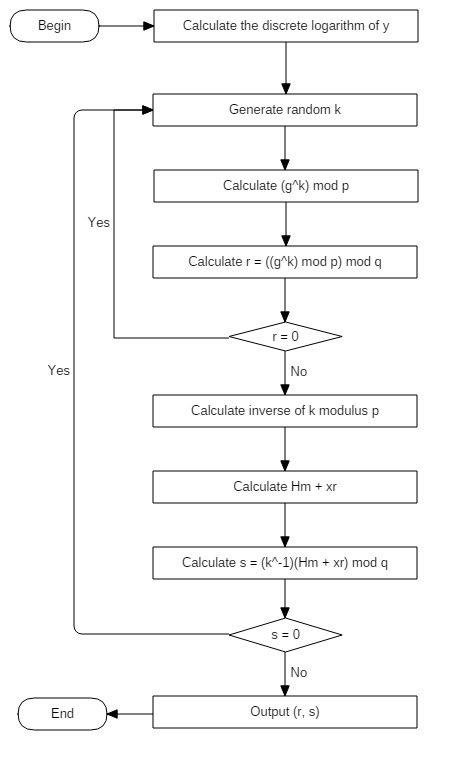
\includegraphics [scale=0.5]{bab2/img/main-diagram}
	\caption {Diagram Alur Penyelesaian Permasalahan}
	\label {fig:main_diagram}
\end{figure}
Terdapat beberapa \textit{bottleneck} pada prosedur pembuatan signature, di antaranya penghitungan logaritma diskret $ y $, penghitungan nilai $g^k\ mod\ p$, dan penghitungan invers $k\ \left(mod\ p\right)$. Selain proses yang telah dipaparkan pada gambar \ref{fig:main_diagram}, terdapat sebuah proses yang merentang di tiap tahapan pembuatan \textit{signature}.

Soal menyiratkan bahwa parameter $p$ memiliki nilai paling tinggi sekitar $2^{60}$ sedangkan pada waktu penulisan, nilai \textit{integer} yang paling besar yang dapat ditampung pada mesin adalah $2^{64}$. Konsekuensi tingginya parameter $p$ adalah akan ada parameter lain yang memiliki batas atas nilai yang tinggi pula. Hal ini dapat menyebabkan masalah pada saat melakukan perkalian.

Perkalian dua nilai yang mendekati $2^{60}$ dapat mengakibatkan \textit{integer overflow}. Maka pada proses perkalian di seluruh tahapan pembuatan \textit{signature}, prosedur perkalian harus menggunakan metode yang dapat menghindari \textit{integer overflow}.

Berdasarkan penjelasan yang telah dijabarkan, hal-hal yang diperlukan untuk menyelesaikan permasalahan DSA Attack adalah sebagai berikut.

\begin{enumerate}
	\item Strategi penghitungan logaritma diskret, akan dibahas pada subbab \ref{sec:Strategi Penyelesaian Logaritma Diskret}.
	\item Strategi pemangkatan modular (penghitungan nilai $ g^k\ mod\ p $), akan dibahas pada subbab \ref{sec:Strategi Penyelesaian Pemangkatan Modular}.
	\item Strategi penghitungan invers $ k\ (mod\ p) $, akan dibahas pada subbab \ref {sec:Strategi Penyelesaian Invers Modulus}.
	\item Strategi perkalian modular (penghitungan nilai $ a * b\ mod\ p $), akan dibahas pada subbab \ref{sec:Strategi Perkalian Modular}.
\end{enumerate}

\section{Strategi Penyelesaian Pemangkatan Modular}
Bagian ini akan menjelaskan beberapa variasi penyelesaian pencarian hasil pemangkatan pada persamaan kongruen yang dijabarkan pada persamaan \eqref{eq:pemangkatan_modular}.
\begin{equation}
h \equiv a^k\ mod\ m,\text{untuk a, k, dan m yang ditentukan}
\label{eq:pemangkatan_modular}
\end{equation}

\subsection{Strategi Penyelesaian Pemangkatan Modular secara Naif}
Pencarian hasil persamaan \eqref{eq:pemangkatan_modular} dapat dicari secara iteratif. Hasil perkalian disimpan pada sebuah variabel sementara, $temp_h$. Nilai $temp_h$ secara berkala dikalikan dengan $a$ sebanyak $k$ kali. Setelah pemangkatan selesai dilakukan, nilai $temp_h$ dimodulus dengan $ m $. Prosedur ini ditunjukkan pada pseudocode \ref{psdo:modex_naive}.

\begin{figure}
\begin{lstlisting}[firstnumber=0]
NAIVE-MODULAR-EXPONENTIATION (a, k, m)
let temp_h = 1
for i = 1 to k
	temp_h = temp_h * a
	temp_h = temp_h mod m
return temp_h
\end{lstlisting}
\caption{Pseudocode Penyelesaian Pemangkatan Modular Secara Naif}
\label{psdo:modex_naive}
\end{figure}

Strategi ini membutuhkan $O(k)$ iterasi. Untuk nilai $k$ yang besar, metode ini tidak cukup baik untuk digunakan mengingat ada tahapan lain yang membutuhkan waktu komputasi yang tinggi. Untuk itu sebuah strategi alternatif akan diajukan pada subbab \ref{sec:Strategi Penyelesaian Pemangkatan Modular dengan Repeated Squaring}.

\subsection{Strategi Penyelesaian Pemangkatan Modular dengan Repeated Squaring}

Metode ini memanfaatkan representasi biner indeks pangkat $k$ dalam melakukan pemangkatan. Diberikan tiga masukan: \textit{generator}, \textit{exponent}, dan $p$ yang mengikuti persamaan \eqref{eq:pemangkatan_modular}.
\begin{equation}
	h \equiv generator^{exponent}\ mod\ p
	\label{eq:pemangkatan_modular_repeated_squaring}
\end{equation}
Gambar \ref{fig:repeated_squaring} menjabarkan prosedur metode ini.
\begin{figure}
	\Centering
	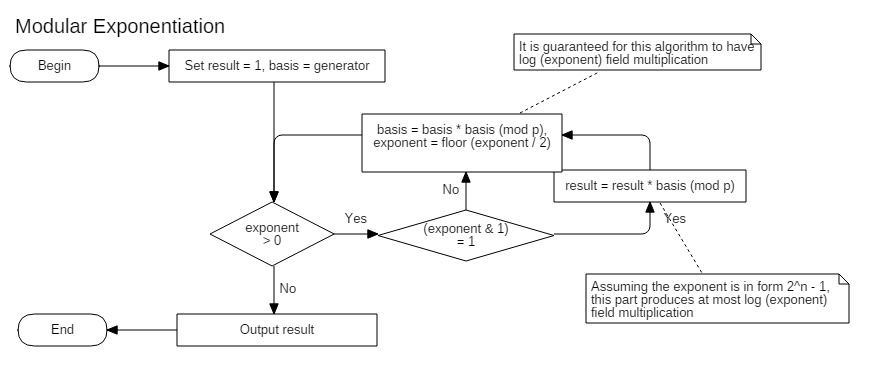
\includegraphics[scale=0.5,angle=90]{bab2/img/modular-exponentiation}
	\caption{Diagram Alur Pemangkatan Modular dengan \textit{Repeated Squaring}}
	\label{fig:repeated_squaring}
\end{figure}

Strategi ini memiliki kompleksitas $O\left(log_2\ p\right)$.

\subsection{Penjelasan Strategi Penyelesaian Pemangkatan Modular dengan Repeated Squaring}

Strategi ini berangkat dari perkalian berulang sebuah nilai $a$ (pada Gambar \ref{fig:repeated_squaring} dinotasikan dengan $ generator $) sebanyak $ k $ (pada Gambar \ref{rig:repeated_squaring} dinotasikan dengan $ exponent $) kali. Dengan kata lain, dibutuhkan $k$ proses perkalian dengan nilai $ a $. Hal ini ditunjukkan pada strategi pemangkatan modular naif. Kendati begitu, ada cara lain dimana walaupun proses pemangkatan membutuhkan $ k $ proses perkalian, pada praktiknya proses perkalian yang terjadi tidak sampai $ k $ kali.

Ide strategi ini adalah dengan memecah pemangkatan menjadi komponen yang lebih kecil. Pemecahan tersebut ditunjukkan pada persamaan \eqref{eq:dekomposisi_eksponen}.
\begin{equation}
a^q = a^{e_1} * a^{e_2} *\ldots*a^{e_n},\ \text{dimana}\ q=e_1+e_2+\ldots+e_n
\label{eq:dekomposisi_eksponen}
\end{equation}

Setelah ini akan dijelaskan mengenai nilai $e_i$. 

Pemangkatan memiliki sifat-sifat operasi layaknya aritmatika pada umumnya, dengan syarat basis pemangkatan harus sama. Strategi ini memanfaatkan sifat perkalian indeks pemangkatan seperti yang ditunjukkan pada persamaan \eqref{eq:dekomposisi_perkalian_indeks_pangkat}.
\begin{equation}
a^r = a^{s*t} = (a^s)^t
\label{eq:dekomposisi_perkalian_indeks_pangkat}
\end{equation}

Substitusi nilai $ s $ menjadi $ \frac{r}{2} $ dan $ t $ menjadi $2$.
\begin{equation}
a^r = a^{\frac{r}{2}*2} = (a^{\frac{r}{2}} )^2
\label{eq:substitusi_indeks_pangkat}
\end{equation}

Penghitungan nilai $ g^{\frac{r}{2}} $ dilakukan dengan menggunakan bentuk persamaan \eqref{eq:substitusi_indeks_pangkat}, hingga didapat nilai $ \displaystyle \frac{r}{2} = 1$. Perkalian secara rekursif ini memiliki jumlah perkalian mengikuti relasi rekurens berikut.
\begin{subequations}
	\[
		O(r)=
		\begin{cases}
			O(1), 			  & \text{if } r = 1 \\
			O(\frac{r}{2}+1), & \text{if } r > 1
		\end{cases}
		\tag{\ref{eq:rekurens_jumlah_perkalian}}
	\]
	\label{eq:rekurens_jumlah_perkalian}
\end{subequations}

Berdasarkan relasi rekurens \eqref{eq:rekurens_jumlah_perkalian}, jumlah perkalian yang dibutuhkan untuk melakukan pemangkatan dengan metode ini adalah $O(log_2\ r)$ dimana $r$ merupakan bilangan pangkat 2.

Telah dijelaskan bagaimana mencari hasil pangkat dimana indeks pangkat $r$ berupa bilangan pangkat 2. Metode pemangkatan dengan \textit{repeated squaring} juga dapat digunakan untuk mencari hasil pangkat dengan indeks pangkat $ r $ bukan bilangan pangkat 2. Pertama, representasi biner dari $ q $ dicari terlebih dahulu. Diberikan sebuah representasi biner r, $ \left\langle a_0,a_1,\dots,a_n\right\rangle $ yang mengikuti persamaan \eqref{eq:dekomposisi_biner}.
\begin{equation}
r = (2^0 * r_0) + (2^1* r_1) + (2^2 * r_2) + \dots + (2^n* r_n)
\label{eq:dekomposisi_biner}
\end{equation}

Nilai $ r $ pada persamaan \eqref{eq:dekomposisi_biner} kemudian dimasukkan ke $ a^r $ menjadi
\begin{align}
a^r &= a^{(2^0 * r_0) + (2^1 * r_1) + (2^2 * r_2) + \dots + (2^n * r_n)} \\
a^r &= a^{2^0 * r_0} * a^{2^1 * r_1} * a^{2^2 * r_2} * \dots * a^{2^n * r_n} \\ 
a^r &= (a^{2^0})^{r_0} * (a^{2^1})^{r_1} * (a^{2^2})^{r_2} * \dots * (a^{2^n})^{r_n} \\
a^r &= (a^1)^{r_0} * (a^2)^{r_1} * (a^4)^{r_2} * \dots * (a^{2^{log_2\ r}})^{r_n} \\
a^r &= y_0^{r_0} * y_1^{r_1} * y_2^{r_2} * \dots * y_n^{r_n},\text{untuk } y_i=a^{2^i}
\label{eq:generalisasi_dekomposisi_biner_pemangkatan}
\end{align}

Persamaan \eqref{eq:generalisasi_dekomposisi_biner_pemangkatan} menunjukkan transformasi penghitungan pemangkatan dengan $ r $ menjadi sederet perkalian. Perlu diperhatikan bahwa penghitungan nilai $ (a^2)^i $ membutuhkan $ O(log_2\ 2^i) $ perkalian. Maka penghitungan $ y_i=a^{2^i} $ juga membutuhkan $ O(log_2\ 2^i) $ perkalian. Dari penjabaran ini, untuk menghitung semua nilai $ y_i $ pada persamaan \eqref{eq:generalisasi_dekomposisi_biner_pemangkatan} membutuhkan perkalian sebanyak
\begin{equation}
\sum_{i=1}^{n} log_2\ {2^i}=\sum_{i=1}^{n} i=\frac{n(n+1)}{2}
\label{eq:jumlah_perkalian_generalisasi_dekomposisi_biner}
\end{equation}

Perhatikan bahwa $ y_0 $ tidak diikutsertakan pada penghitungan karena $ y_0=a^{2^0}=a^1 $, sehingga tidak dibutuhkan perkalian apapun. Total perkalian yang dibutuhkan untuk menghitung $ y_i=a^{2^i} $ pada persamaan \eqref{eq:generalisasi_dekomposisi_biner_pemangkatan} adalah $ \frac{n(n+1)}{2} \in O(n^2) $. Metode ini tentu tidak lebih baik dari metode pemangkatan naif dimana dibutuhkan $ O\left(n\right) $ perkalian. Maka dari itu perlu dilakukan perubahan mengenai cara penghitungan $ y_i $.

Untuk menekan jumlah perkalian, penghitungan $ y_i $ dapat diubah menjadi relasi rekurens \eqref{eq:relasi_rekurens_y_i}.
\begin{subequations}
	\[
		y_i=
		\begin{cases}
			a, 		   & \text{if } i = 0 \\
			y_{i-1}*a, & \text{if } i > 0
		\end{cases}
		\tag{\ref{eq:relasi_rekurens_y_i}}
	\]
	\label{eq:relasi_rekurens_y_i}
\end{subequations}

Untuk mencari nilai $ y_i $, cukup menggunakan nilai $ y_{i-1} $ dan dikalikan dengan $ a $. Konsekuensi yang dimiliki cara ini adalah nilai $ y_i $ dapat digunakan untuk mendapatkan nilai $ y_{i+1} $. Maka sebetulnya untuk menghitung nilai $ y_i $, tidak perlu menghitung dari $ y_0 $. Apabila nilai $ y_{i-1} $ sudah diketahui, cukup mengalikan nilai tersebut dengan $ a $.

Pemanfaatan relasi rekurens \eqref{eq:relasi_rekurens_y_i} dapat dilakukan dengan menggunakan nilai $ y_i $ dan variabel $ temp $ yang berfungsi untuk menyimpan hasil perkalian. Mulai dari $ i=0 $, pangkatkan $ y_i $ dengan $ r_i $. Pemangkatan ini hanya memiliki dua hasil seperti yang ditunjukkan pada persamaan \eqref{eq:hasil_relasi_rekurens_y_i}.
\begin{subequations}
	\[f_y(i)=
		\begin{cases}
			1,  & \text{if } r_i=0 \\
			y_i,& \text{if } r_i=1
		\end{cases}
		\tag{\ref{eq:hasil_relasi_rekurens_y_i}}
	\]
	\label{eq:hasil_relasi_rekurens_y_i}
\end{subequations}
Hasil pemangkatan (yaitu nilai $ f_y(i) $) digabungkan ke $ temp $ dengan cara dikalikan.

Dari penjabaran tersebut, penghitungan persamaan \eqref{eq:generalisasi_dekomposisi_biner_pemangkatan} dengan metode ini membutuhkan hanya satu kali perhitungan nilai $ y_i $, yaitu penghitungan $ y_i $ pada $ i=n $. Proses penghitungan $ y_n $ juga menghitung nilai $ y_0 $ hingga $ y_{n-1} $. Sehingga dengan menghitung $ y_n $, nilai $ y_0 $ hingga $ y_{n-1} $ juga didapat. Jumlah perkalian menggunakan relasi rekurens \eqref{eq:relasi_rekurens_y_i} adalah $ O(n) $ dimana $ n=log_2\ r$ untuk sebuah indeks pangkat $ r $ (atau bisa ditulis $ O\left(log_2\ (r)\right) $). Cara pemangkatan ini lebih cepat dibandingkan cara pemangkatan naif.

\section{Strategi Penyelesaian Invers Modulus}

Permasalahan pencarian invers modulus adalah mencari nilai $ a' $ pada persamaan \eqref{eq:persamaan_umum_invers_modulus}.
\begin{equation}
a * a' \equiv 1\ (mod\ m), \text{untuk nilai a dan m tertentu}
\label{eq:persamaan_umum_invers_modulus}
\end{equation}
Invers modulus adalah analog dari pembagian pada $ \mathbb{Z}_n $.

Sebelum mencari nilai $ a' $, hal yang perlu diketahui terlebih dahulu adalah apakah benar ada nilai $ a' $ yang bisa membuat persamaan \eqref{eq:persamaan_umum_invers_modulus} bernilai benar. Pertanyaan ini bisa dijawab dengan menggunakan Identitas Bezout.

\subsection{Identitas Bezout}

Identitas Bezout berbicara mengenai persamaan berkaitan dengan faktor persekutuan terbesar dua bilangan \cite{brilliant_bezout}. Notasi yang digunakan untuk menyatakan faktor persekutuan terbesar dapat dilihat pada persamaan \eqref{eq:gcd}.
\begin{equation}
\gcd⁡(a,b)=\max R,\ R=\left\{r:r|a\ \text{dan} \ r|b\right\}
\label{eq:gcd}
\end{equation}

Identitas Bezout adalah sebuah persamaan yang menghasilkan faktor persekutuan terbesar dua bilangan.
\begin{equation}
ax+by=\gcd(a,b), \text{untuk nilai a dan b tertentu}
\label{eq:identitas_bezout}
\end{equation}
Sisi kanan persamaan \eqref{eq:identitas_bezout} tidak akan memiliki nilai kurang dari $ \gcd (a,b) $. Dengan kata lain nilai terkecil bukan nol yang mungkin untuk sisi kanan persamaan \eqref{eq:identitas_bezout} adalah $ \gcd (a,b) $.

Kembali ke persamaan \eqref{eq:persamaan_umum_invers_modulus}, Identitas Bezout menjamin adanya sebuah nilai $ a' $ yang menyebabkan persamaan \eqref{eq:persamaan_umum_invers_modulus} bernilai benar dengan syarat $ \gcd (a,m) = 1 $. Pembuktian klaim ini dapat dilihat pada penjabaran berikut.
\begin{align}
a * a' &\equiv 1\ (mod\ m) \\
aa' &= qm + 1 \\
1 &= aa' + (-q)m
\label{eq:proof_bezout_koprima}
\end{align}
Persamaan \eqref{eq:proof_bezout_koprima} memiliki bentuk persamaan \eqref{eq:identitas_bezout}. Sisi kiri persamaan \eqref{eq:proof_bezout_koprima} merupakan sisi kanan persamaan \eqref{eq:identitas_bezout}, atau dengan kata lain $ \gcd (a, m) = 1 $. Perhatikan bahwa hasil akhir penjabaran di atas merupakan persamaan \eqref{eq:identitas_bezout}, yaitu Identitas Bezout. Dari sini dapat disimpulkan bahwa $ \gcd (a, m)=1 $. Artinya syarat untuk sebuah nilai $ a $ memiliki invers modulus adalah $ a $ harus koprima dengan modulus $ m $. \hfill $ \eop $

\subsection{Strategi Penyelesaian Invers Modulus secara Naif}

Pencarian invers modulus dapat dilakukan dengan \textit{brute force}. Semua nilai $ a' $ dicoba dan diperiksa apakah hasil perkalian persamaan \eqref{eq:persamaan_umum_invers_modulus} menghasilkan $ 1\ (mod\ m) $. Gambar \ref{psdo:modinv_naive} memaparkan langkah yang dijelaskan.
\begin{figure}[h!]
\begin{lstlisting}[firstnumber=0]
NAIVE-MODULAR-INVERSE (a, m)
if gcd(a,m) != 1
	return “NOT INVERTIBLE”
for a' = 1 to m-1
	if (a * a') mod m == 1
		return a'
\end{lstlisting}
\caption{Pseudocode Pencarian Modular Invers Naif}
\label{psdo:modinv_naive}
\end{figure}

Strategi ini membutuhkan $ O(m) $ percobaan. Strategi ini mudah untuk diimplementasikan karena cukup mencoba nilai $ a' $ satu per satu hingga ditemukan nilai $ a' $ yang memenuhi persamaan \eqref{eq:persamaan_umum_invers_modulus}. Untuk mereduksi daerah pencarian, pencarian invers modulus dapat dibatasi supaya hanya dilakukan untuk pasangan $ a $ dan $ m $ dimana $ \gcd⁡(a, m)= 1 $. Untuk $ m $ yang besar, strategi ini tidak cukup baik untuk digunakan mengingat masih ada proses lain yang membutuhkan waktu komputasi yang tinggi. Maka dari itu, strategi lain yang lebih baik akan dijabarkan pada subbab selanjutnya.

\subsection {Strategi Penyelesaian Invers Modulus dengan Extended Euclidean}

Strategi ini memanfaatkan Identitas Bezout, yaitu mencari nilai $ a $ dan $ b $ untuk $ x $ dan $ y $ tertentu pada persamaan \eqref{eq:identitas_bezout}. Gambar \ref{psdo:extended_euclidean} merupakan pseudocode yang menggambarkan metode pencarian invers modulus menggunakan \textit{Extended Eucliean}.

\begin{figure}[h!]
\begin{lstlisting}[firstnumber=0]
MODULAR-INVERSE-WITH-EXTENDED-EUCLIDEAN (a = qb + r)
let EQUATION[] be a new array
let i = 0
while r != 0
	EQUATION[i] = (a = qb + r)
	find equation b = qr + m for some q and m
	i = i + 1
for i = EQUATION.len – 1 downto 1
	substitute EQUATION[i].b with EQUATION[i+1].r
return (EQUATION[1].x, EQUATION[1].y)
\end{lstlisting}
\caption{Pseudocode \textit{Extended Euclidean}}
\label{psdo:extended_euclidean}
\end{figure}

Strategi ini membutuhkan $ O((log_2\ n)^2) $ operasi bit. \cite{hac_math}

\subsection{Penjelasan Strategi Penyelesaian Invers Modulus dengan Extended Euclidean}

Ide strategi ini adalah dengan mentransformasi nilai $ a $ dan $ b $ menjadi sebuah nilai dimana $ a $ habis dibagi oleh $ b $. Tiap langkah transformasi akan ditulis menggunakan persamaan \eqref{eq:persamaan_umum_pembagian}, yaitu bentuk umum pembagian.
\begin{equation*}
a=qb+r
\end{equation*}

Persamaan \eqref{eq:persamaan_umum_pembagian} diberi batasan, yaitu nilai $ r $ harus kurang dari $ b $. Langkah transformasi adalah sebagai berikut.
\begin{enumerate}
\item Cari nilai $ q $ dan $ r $ yang memenuhi persamaan \eqref{eq:persamaan_umum_pembagian}.
\item Simpan nilai $ a, b, q, $ dan $ r $ sebagai nilai persamaan iterasi ke-i.
\item Cari bentuk persamaan \eqref{eq:persamaan_umum_pembagian} untuk $ b $ dengan cara melakukan modulus $ b $ dengan $ r $
\item Ulangi langkah 2 hingga ditemukan $ r $ bernilai 0.
\end{enumerate}

Tabel \ref{tab:transformasi_ext_euclid} mengilustrasikan langkah ini. Diberikan $ a = 97 $ dan $ b = 35 $. Nilai $ q $ sengaja tidak dimasukkan pada kolom \textit{persamaan} untuk memperjelas bentuk persamaan \eqref{eq:persamaan_umum_pembagian}
\begin{table}[h!]
\Centering
\caption{Contoh Proses Transformasi}
\label{tab:transformasi_ext_euclid}
\begin{tabular}{ |l|l|l|l|l|l| }
	\hline
	Iterasi	& a		& b		& r		& q		& Persamaan \\
	\hline
	1		& 97	& 35	& 27	& 2		& $ 97 = 35 * q + 27 $ \\
	2		& 35	& 27	& 8		& 1		& $ 35 = 27 * q + 8 $ \\
	3		& 27	& 8		& 3		& 3		& $ 27 = 8 * q + 3 $ \\
	4		& 8		& 3		& 2		& 2		& $ 8 = 3 * q + 2 $ \\
	5		& 3		& 2		& 1		& 1		& $ 3 = 2 * q + 1 $ \\
	6		& 2		& 1		& 0		& 2		& $ 2 = 1 * q + 0 $ \\
	\hline
\end{tabular}
\end{table}

Pada iterasi 6, didapat nilai $ r = 0 $. Maka proses transformasi berhenti pada iterasi ini. Kemudian, dengan persamaan yang telah terbentuk di tiap iterasi, setiap persamaan dapat diangkat ke persamaan pada satu iterasi sebelumnya dengan cara substitusi. Berikut contoh pengangkatan iterasi 6 ke iterasi 5.
\begin{align}
2 &=1(2)+0 \label{eq:contoh_pengangkatan_1} \\
0 &=2-1(2) \label{eq:contoh_pengangkatan_2} \\
0 &=2-(3-2(1))(2) \label{eq:contoh_pengangkatan_3} \\
0 &=2-3(2)+2(2) \label{eq:contoh_pengangkatan_4} \\
0 &=2(3)-3(2) \label{eq:contoh_pengangkatan_5}
\end{align}

Hasil akhir pengangkatan tersebut (persamaan \eqref{eq:contoh_pengangkatan_5}) adalah bentuk persamaan pada iterasi 5, hanya saja nilai pada sisi kiri persamaan tertambah perkalian dengan 2 (persamaan \eqref{eq:contoh_pengangkatan_5} dapat ditulis menjadi $ 3(2)=2(2)+0 $).

Perhatikan penggunaan tanda kurung pada proses pengangkatan. Nilai pada tanda kurung bermakna variabel, sedangkan nilai yang berada di luar kurung bermakna koefisien. Pada proses pengangkatan, substitusi persamaan dengan persamaan pada iterasi lain hanya boleh dilakukan pada koefisien. Namun, penyederhanaan persamaan tidak boleh mengubah konstanta. Artinya, penyederhanaan persamaan hanya bekerja pada variabel.

Di baris ketiga contoh pengangkatan (persamaan \eqref{eq:contoh_pengangkatan_3}) merupakan proses substitusi. Nilai $ 1 $ diubah menjadi $ 3-2(1) $. Kemudian, dilakukan distribusi untuk mengeluarkan persamaan substitusi dari kurung. Pada baris kelima contoh pengangkatan di atas merupakan proses penyederhanaan. Perhatikan bagaimana nilai $ 2 $ tidak digabungkan ke $ 3(2) $, melainkan ke $ 2(2) $. Hal ini disebabkan nilai $ 3(2) $ memiliki koefisien $ 3 $, sedangkan nilai yang akan digabungkan memiliki koefisien $ 2 $. Untuk itu, nilai $ 2 $ dimasukkan ke nilai yang sama-sama memiliki koefisien $ 2 $.

Pengangkatan dilakukan dari iterasi sebelum iterasi terakhir. Pada contoh di atas, iterasi terakhir terdapat pada iterasi ke-6. Maka iterasi sebelum iterasi terakhir adalah iterasi ke-5. Hal ini bertujuan agar persamaan \eqref{eq:identitas_bezout} terpenuhi. Proses pengangkatan dilakukan hingga iterasi pertama.

Langkah seluruh pengangkatan dapat dijabarkan sebagai berikut.
\begin{enumerate}
\item Ubah semua persamaan $ a=qb+r $ menjadi $ r=a-qb $.
\item Substitusi nilai $ b $ pada iterasi sekarang dengan nilai $ r $ pada iterasi selanjutnya.
\item Lakukan penyederhanaan dengan menggabungkan konstanta yang sama
\item Ulangi langkah 2 dan 3 hingga seluruh iterasi telah dilewati.
\end{enumerate}

Tabel \ref{tab:pengangkatan_ext_euclid} berisi contoh pengangkatan berdasarkan hasil transformasi sebelumnya.

\begin{table}[h!]
\small
\Centering
\caption{Contoh Proses Pengangkatan}
\label{tab:pengangkatan_ext_euclid}
\begin{tabular} { |l|l|l|l|l|l|l| }
	\hline
	Iterasi	& a		& b		& r		& q		& Persamaan			& Pers. Akhir \\
	\hline
	5		& 3		& 2		& 1		& 1		& $ 1 = 3 - 2(1) $		& $ 1 = 3 - 2(1) $ \\
	4		& 8		& 3		& 2		& 2		& $ 2 = 8 - 3(2) $		& $ 1 = 3(3) - 8(1) $ \\
	3		& 27	& 8		& 3		& 3		& $ 3 = 27 - 8(3) $ 	& $ 1 = 27(3) - 8(10) $ \\
	2		& 35	& 27	& 8		& 1		& $ 8 = 35 - 27(1) $	& $ 1 = 27(13) - 35(10) $ \\
	1		& 97	& 35	& 27	& 2		& $ 27 = 97 - 35(2) $	& $ 1 = 97(13) - 35(36) $ \\
	\hline
\end{tabular}
\end{table}

Maka didapat persamaan akhir $ 1=97(13)-35(36) $. Persamaan ini dapat ditulis agar mengikuti persamaan \eqref{eq:identitas_bezout}. Penulisan persamaan tersebut yaitu $ 1=97(13)-35(36) \Rightarrow 1=97(13)+35(-36) $. Pasangan setiap konstanta -- variabel merupakan invers untuk satu sama lain. $ 97 $ merupakan invers dari $ 13 $, dan $ 35 $ merupakan invers dari $ -36 $. Seringkali nilai invers yang diinginkan berupa nilai positif. Untuk mengatasi hal itu, cukup mencari kelas residu dari $ -36 $. Pada kasus ini $ -36\in[3]_{13}$ dan $ -36\in[61]_{97} $. Maka $ -36\equiv3\ (mod\ 13) $ dan $ -36\equiv61\ (mod\ 97) $.
Efisiensi strategi ini jauh lebih baik daripada strategi naif.

\section{Strategi Penyelesaian Logaritma Diskret}

Permasalahan logaritma diskret adalah mencari nilai $ x $ pada persamaan \eqref{eq:persamaan_umum_log_diskret}
\[
y \equiv g^{x}\ (mod\ n),\text{untuk nilai y, g dan n tertentu}
\]

Penghitungan nilai logaritma diskret menjawab dua pertanyaan:
\begin{enumerate}
\item Apakah ada sebuah nilai $ x $ yang bisa menyebabkan persamaan \eqref{eq:persamaan_umum_log_diskret} benar?
\item Nilai $ x $ apa yang mampu membuat persamaan \eqref{eq:persamaan_umum_log_diskret} benar?
\end{enumerate}

Pertanyaan 1 membutuhkan ulasan yang panjang. Penyebab panjangnya ulasan ini adalah ada permutasi $ g $, $ n $, dan $ y $ yang tidak menjamin terdapat nilai $ x $ yang bisa menyebabkan persamaan \eqref{eq:persamaan_umum_log_diskret} benar. Kendati begitu, pertanyaan 1 dapat dijawab secara ringkas dengan memperhatikan penjelasan soal. 

Sebelumya disebutkan bahwa permutasi $ g $, $ n $, dan $ y $ menentukan ada atau tidaknya nilai $ x $ yang sesuai. Pada soal disebutkan bahwa parameter \textit{private key} dan \textit{public key} yang diberikan dijamin dibentuk dengan langkah berikut.

\begin{enumerate}
\item Tentukan sebuah nilai $ x $ secara acak dimana $ 0 < x < q $.
\item Hitung $ y = g^x\ (mod\ p) $.
\item \textit{Public key} adalah $ (p, q, g, y) $, dan \textit{private key} adalah $ x $.
\end{enumerate}

Artinya untuk \textit{public key} $ (p, q, g, y) $ dijamin terdapat sebuah \textit{private key} $ x $ yang cocok dengan \textit{public key} tersebut. Maka persamaan \eqref{eq:persamaan_umum_log_diskret} dijamin memiliki sebuah nilai $ x $ yang menyebabkan persamaan tersebut benar. Pertanyaan berikutnya adalah nilai $ x $ apa yang memenuhi persamaan \eqref{eq:persamaan_umum_log_diskret} (yaitu pertanyaan 2).

Bab ini akan menjelaskan beberapa variasi penyelesaian logaritma diskret. Sebelum itu, perlu dijelaskan beberapa hal yang digunakan untuk menyelesaikan permasalahan logaritma diskret.

\subsection {Teorema Euler}

Teorema Euler berbicara mengenai periodisitas nilai hasil pemangkatan pada persamaan kongruensi. Teorema Euler menggunakan sebuah fungsi yang disebut \textit{Euler Totient Function}.\cite{stallings_cryptography}
\begin{equation}
\phi(n)=\left|S\right|, \text{dimana } S=\left\{r\ :\ \gcd (r,n)=1; 0 < r < n \right\}
\label{eq:euler_totient_function}
\end{equation}
Perhatikan bahwa apabila $ n $ merupakan bilangan prima, maka $ \phi(n)=n-1 $.

Teorema Euler dapat ditulis sebagai berikut. Diketahui terdapat dua nilai: sebuah basis pangkat $ a $, dan sebuah modulus $ n $
\begin{equation}
a^{\phi(n)}\equiv 1\ (mod\ n), \qquad \gcd(a,n)=1
\label{eq:teorema_euler}
\end{equation}

Persamaan \eqref{eq:teorema_euler} menjelaskan bahwa sebuah bilangan $ a $ dimana $ a $ koprima dengan $ n $, apabila dipangkatkan dengan $ \phi(n) $ akan menghasilkan nilai $ t \in [1]_n $. Artinya, $ a^{\phi(n)}\ mod\ n=1 $. Maksud persamaan \eqref{eq:teorema_euler} adalah apabila perkalian dengan $ a $ diulang sebanyak $ \phi(n) $ kali dimana $ n $ adalah modulus yang digunakan, semua nilai yang mungkin dari perkalian modular tersebut telah dihasilkan. Perkalian lebih lanjut hanya akan mengulang nilai-nilai tersebut.

Persamaan \eqref{eq:teorema_euler} tidak menjamin seluruh anggota himpunan $ \mathbb{Z}_n^{*}=\left\{ i : 1 \leq i < n\right\} $ telah dihasilkan. Apa yang dijamin oleh persamaan \eqref{eq:teorema_euler} adalah terdapat sebuah himpunan $ \mathbb{H}_{(a,n)} $ yang memenuhi persamaan \eqref{eq:himpunan_Ha}.
\begin{equation}
\mathbb{H}_{(a,n)}=\left\{a^{i}\ (mod\ n)\ :\ 0 \leq i < \phi(n) \right\}
\label{eq:himpunan_Ha}
\end{equation}
$ \mathbb{H}_{(a, n)} $ dapat didefinisikan sebagai sebuah himpunan yang anggotanya adalah semua nilai yang dapat dibentuk dari $ a^i (\ mod\ n) $ untuk seluruh nilai $ i $. Pada proses pemangkatan $ a^{\phi(n)} $, seluruh anggota himpunan $ \mathbb{H}_{(a, n)} $ telah dihasilkan.

Himpunan $ \mathbb{H}_{(a, n)} $ tidak selalu sama dengan himpunan $ \mathbb{Z}_n^{*} $. Kasus yang menggambarkan pernyataan ini yaitu pemangkatan pada persamaan kongruensi modulo 7, dimana $ \phi(7)=\left|\left\{1,2,3,4,5,6\right\}\right|\allowbreak=6 $. Dengan mengambil contoh $ a=6 $, didapat bahwa himpunan $ \mathbb{H}_{(a=6,n=7)}=\left\{1,6,1,6,1,6\right\} $. Penjelasan lebih lanjut mengenai perbedaan himpunan $ \mathbb{H}_{(a, n)} $ dengan $ \mathbb{Z}_n^{*} $ akan dijabarkan pada bab \ref{sec:Order Sebuah Elemen}.

Persamaan \eqref{eq:teorema_euler} dapat diubah menjadi bentuk logaritmik.
\begin{align}
a^{\phi(n)} &\equiv 1\ (mod\ n) \\
a^{\phi(n)} &\equiv a^0\ (mod\ n) \\
\phi(n) &\equiv 0\ (mod\ \phi(n))
\label{eq:teorema_euler_logaritmik}
\end{align}

Perhatikan perubahan persamaan \eqref{eq:teorema_euler} menjadi \eqref{eq:teorema_euler_logaritmik} mengubah nilai modulus. Hal ini disebabkan terdapat perubahan domain dimana persamaan \eqref{eq:teorema_euler_logaritmik} bekerja, yaitu dari domain hasil pemangkatan menjadi domain indeks pangkat. Teorema Euler memicu perubahan nilai modulus, dimana pemangkatan sebuah bilangan dengan $ \phi(n) $ bermakna sama dengan pemangkatan sebuah bilangan dengan $ 0 $. Penjelasan ini merupakan definisi persamaan \eqref{eq:teorema_euler_logaritmik}.

\subsection{Order Sebuah Elemen}

Definisi order sebuah elemen $ a $ adalah sebuah nilai $ h $ positif terkecil dimana apabila $ a $ dioperasikan dengan $ a $ sebanyak $ h $ kali akan menghasilkan elemen identitas operasi $ e $.\cite{harald_applied_number_theory}
\begin{equation}
ord(a)=h,\text{ dimana }\underbrace{a\cdot a\cdot\ldots\cdot a\cdot a}_{\text{h operasi}}=e
\label{eq:order_elemen}
\end{equation}

Definisi ini terlalu luas untuk digunakan pada permasalahan logaritma diskret. Untuk itu, definisi tersebut bisa dipersempit: Order sebuah elemen $ a $ adalah suatu nilai $ h $ positif terkecil dimana apabila $ a $ dipangkatkan dengan $ h $ akan menghasilkan $ 1\ (mod\ n) $. Secara formal, penjelasan ini dapat ditulis menjadi persamaan \eqref{eq:order_modular_elemen}.
\begin{equation}
a^h\equiv 1\ (mod\ n)
\label{eq:order_modular_elemen}
\end{equation}

Apabila sebuah elemen $ a $ memiliki order senilai $ \phi(n) $, elemen tersebut dinamakan \textit{primitive root modulo n}.
Perhatikan bahwa persamaan \eqref{eq:order_modular_elemen} mirip dengan persamaan \eqref{eq:teorema_euler}. Kedua persamaan tersebut mengimplikasikan bahwa $ h\ |\ \phi(n) $ atau $ \phi(n) $ merupakan kelipatan $ h $, untuk $ h\leq \phi(n) $. Pembuktian klaim tersebut dapat dilihat pada penjabaran persamaan \eqref{eq:proof_order_modular_elemen_begin} sampai \eqref{eq:proof_order_modular_elemen}.

Pertama asumsikan sebuah nilai $ g $ yang memiliki order sebesar $ h $ pada \textit{group} $ \mathbb{Z}_n $, dan sebuah \textit{primitive root} $ a $.
\begin{align}
\label{eq:proof_order_modular_elemen_begin}
a^{\phi(n)} &\equiv 1\ (mod\ n)	\\
a^{\phi(n)} &\equiv g^h\ (mod\ n) \\
\phi(n) &\equiv (\log_a g) * h\ (mod\ \phi(n)) \\
0 &\equiv (\log_a {a^x}) * h\ (mod\ \phi(n)) \\
0 &\equiv x * h\ (mod\ \phi(n))
\label{eq:proof_order_modular_elemen}
\end{align}

Pada subbab \ref{sec:Teorema Euler} telah dijelaskan mengenai himpunan $ \mathbb{H}_{(a, n)} $ (perhatikan kembali persamaan \eqref{eq:himpunan_Ha}) dan bagaimana himpunan $ \mathbb{H}_{(a, n)} $ tidak selalu sama dengan himpunan $ Z_n^* $. Hal ini berhubungan dengan sifat \textit{order} $ h $, yaitu $ h\ |\ \phi(n) $. Sifat ini dapat ditulis menjadi persamaan \eqref{eq:sifat_himpunan_Ha}.
\begin{equation}
\phi(n)=x*h,\text{untuk x tertentu}
\label{eq:sifat_himpunan_Ha}
\end{equation}
Kemudian dengan memasukkan \textit{primitive root} ke persamaan \eqref{eq:sifat_himpunan_Ha}, didapat persamaan \eqref{eq:proof_kesamaan_euler_phi_omega}.
\begin{align}
a^{\phi(n)} &=a^{xh} \\
a^{\phi(n)} &=(a^x)^h \\
a^{\phi(n)} &=\omega^h
\label{eq:proof_kesamaan_euler_phi_omega}
\end{align}
Maka dari penjabaran di atas, sebuah elemen $ a $ yang memiliki order $ h $ (yaitu $\omega$) sebenarnya adalah sebuah \textit{primitive root} yang telah dipangkatkan dengan suatu nilai $ x $.\hfill\eop

Himpunan $ \mathbb{H}_{(\omega, n)} $ adalah semua nilai yang dapat dibentuk oleh $ a^{xi} $ untuk $ 0\leq i < \frac{\phi(n)}{x} \Rightarrow 0\leq i < h $. Artinya, anggota $ \mathbb{H}_{(\omega, n)} $ hanyalah nilai yang dapat dibentuk oleh pangkat kelipatan $ x $. Nilai lain bukan merupakan anggota himpunan $ \mathbb{H}_{(\omega, n)} $. Secara formal penjelasan ini dapat ditulis menjadi persamaan \eqref{eq:himpunan_Hw}.
\begin{equation}
\mathbb{H}_{(\omega,n)}=\left\{\omega^i\ (mod\ n)\ :\ 0 \leq i \leq \frac{\phi(n)}{h}\right\}
\label{eq:himpunan_Hw}
\end{equation}
dimana $ \omega=a^h $ untuk $ a $ sebuah \textit{primitive root modulo n} dan $ h $ tertentu.

Dari pemaparan di atas, hubungan himpunan $ \mathbb{Z}_n^* $, $ \mathbb{H}_{(a, n)} $ dimana $ a $ sebuah \textit{primitive root}, dan $ \mathbb{H}_{(\omega, n)} $ dimana $ \omega $ sebuah elemen dengan order $ h $ dapat dilihat pada relasi \eqref{eq:relasi_zn_ha_hw}.
\begin{equation}
\mathbb{Z}_n^*\supseteq \mathbb{H}_{(a, n)} \supseteq \mathbb{H}_{(\omega, n)}
\label{eq:relasi_zn_ha_hw}
\end{equation}

$ \mathbb{H}_{(a, n)} $ akan sama dengan $ \mathbb{Z}_n^* $ apabila $ a $ merupakan \textit{primitive root}. $ \mathbb{H}_{(\omega, n)} $ akan sama dengan $ \mathbb{H}_{(a, n)} $ apabila order $ {\omega} $ adalah $ \phi(n) $.

\subsection{Strategi Penyelesaian Naif Untuk Logaritma Diskret}
Pencarian nilai $ x $ pada persamaan \eqref{eq:persamaan_umum_log_diskret} bisa dilakukan dengan mencoba semua nilai $ x = 0 $ hingga $ n-1 $. Hitung setiap nilai $ g^x\ (mod\ n) $ dan bandingkan dengan $ y $. Apabila keduanya bernilai sama, maka nilai $ x $ tersebut merupakan nilai logaritma diskret dari $ y $. Gambar \ref{psdo:disc_log_naive} menggambarkan prosedur yang dijelaskan.
\begin{figure}[h!]
\begin{lstlisting}[firstnumber=0]
NAIVE-DISCRETE-LOGARITHM (g, y, n)
result = 1
for i = 0 to n-1
	if result == y
		return i
	result = (result * g) mod n
return "NOT FOUND"
\end{lstlisting}
\caption{Pseudocode Pencarian Logaritma Diskret Secara Naif}
\label{psdo:disc_log_naive}
\end{figure}
Strategi ini memiliki kompleksitas sebesar $ O(n) $.

Metode ini tidak begitu baik apabila $ n $ bernilai besar. Untuk itu, domain $ i $ dapat diperkecil. Karena $ g $ memiliki \textit{order} sebesar $ q $, maka \textit{brute force} dilakukan dengan memangkatkan $ g $ dengan $ i $ dimana $ 0\leq i < ord(g) $ atau $ 0 \leq i < q $ karena semua nilai yang mungkin dibentuk oleh pemangkatan dengan basis $ g $ berada pada rentang tersebut. Pengecilan domain $ i $ menyebabkan kompleksitas metode ini turun menjadi $ O(q) $. Walau telah dilakukan peningkatan, metode ini masih membutuhkan waktu yang relatif besar. Untuk itu alternatif strategi lain akan diajukan pada subbab berikutnya.

\subsection {Strategi Penyelesaian Logaritma Diskret dengan Baby-step Giant-step}
Penyelesaian ini memanfaatkan metode \textit{Baby-step Giant-step} dimana metode ini bertujuan memperkecil daerah pencarian hingga $ \sqrt{n} $ dimana $ n $ merupakan order sebuah elemen $ g $. Gambar \ref{fig:bsgs} memaparkan cara kerja metode ini.

\begin{figure}
	\Centering
	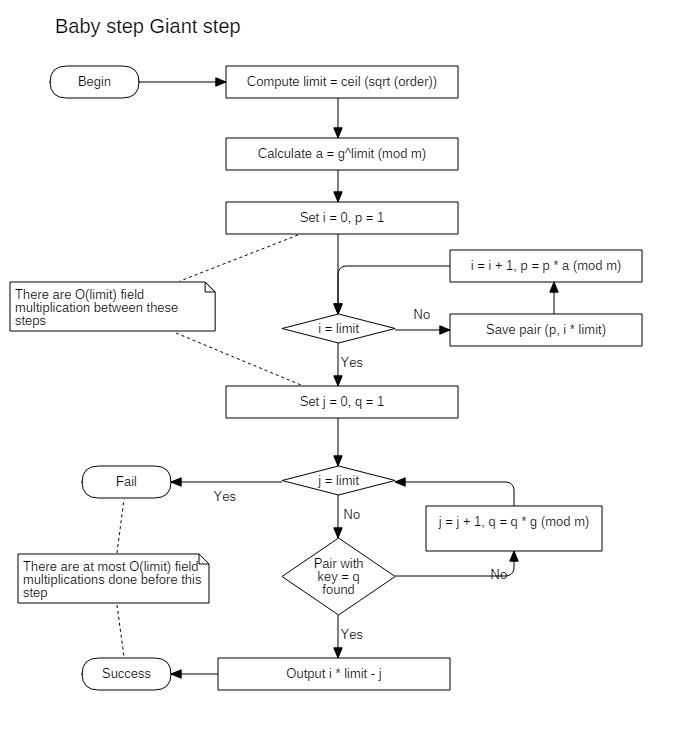
\includegraphics[scale=0.44]{bab2/img/bsgs}
	\caption{Diagram Alur Metode Penyelesaian Logaritma Diskret dengan \textit{Baby-step Giant-Step}}
	\label{fig:bsgs}
\end{figure}

Kompleksitas strategi ini bergantung pada metode pencarian di percabangan kedua ("\textit{pair with key = q found}"). Umumnya metode ini menggunakan metode pencarian \textit{binary search}. Konsekuensinya, penyimpanan pasangan \textit{(p, i * limit)} dilakukan secara terurut dan seluruh proses ini membutuhkan waktu $ O(\sqrt{n}\ log\ n) $. Kemudian dengan menggunakan \textit{binary search} pencarian dapat dilakukan dengan kompleksitas $ O(log\ n) $. Selain \textit{binary search}, dapat juga digunakan \textit{hash table} sebagai alternatif dimana pencarian dapat dilakukan selama $ O(1) $. Penggunaan salah satu dari kedua metode pencarian tersebut mengakibatkan kompleksitas metode \textit{Baby-step Giant-step} secara keseluruhan menjadi $ O(\sqrt{n}) $.

\subsection {Penjelasan Strategi Penyelesaian Logaritma Diskret dengan Baby-step Giant-step}

Persamaan \eqref{eq:persamaan_umum_pembagian} mendasari metode \textit{Baby-step Giant-step}, yaitu pembagian dua bilangan. Diberikan sebuah bilangan $ a $, apabila dibagi dengan sebuah bilangan tertentu $ x $, akan membentuk persamaan \eqref{eq:persamaan_dasar_bsgs}
\begin{equation}
a=qx+r
\label{eq:persamaan_dasar_bsgs}
\end{equation}

Pada persamaan \eqref{eq:persamaan_dasar_bsgs}, $ q $ berada pada rentang $ 0 \leq q \leq a $ dan $ r $ berada pada rentang 
$ 0 \leq r < x $. Umpamakan proses pencarian $ q $ dan $ r $ tidak dapat dilakukan dengan operasi pembagian dan mod. Pencarian nilai $ q $ dan $ r $ maka harus menggunakan pendekatan \textit{brute force}, yaitu mencoba semua kombinasi $ q $ dan $ r $ yang menyebabkan persamaan \eqref{eq:persamaan_dasar_bsgs} bernilai benar. Mengingat nilai $ q $ dan $ r $ bergantung pada nilai $ x $ yang digunakan, maka perlu dipilih sebuah nilai $ x $ yang menyebabkan daerah pencarian $ q $ dan $ r $ minimal. Variabel pada persamaan \eqref{eq:persamaan_dasar_bsgs} yaitu $ q $, $ x $, dan $ r $ memiliki hubungan satu sama lainnya. Hubungan ini dapat dilihat pada proporsi \eqref{eq:proporsi_var_persamaan_dasar_bsgs}.
\begin{equation}
\frac{1}{q} \propto x \propto r
\label{eq:proporsi_var_persamaan_dasar_bsgs}
\end{equation}

Variabel $ q $ dan $ x $ memiliki proporsi saling terbalik, yaitu apabila nilai $ q $ naik, nilai $ x $ akan turun. Kasus sebaliknya juga berlaku. Sedangkan variabel $ x $ dan $ r $ memiliki proporsi langsung, yaitu apabila nilai $ x $ naik, nilai $ r $ akan naik juga. Kasus sebaliknya juga berlaku. Untuk menghasilkan kombinasi $ q $ dan $ r $ yang minimal, nilai $ x $ harus dipilih supaya $ q $ dan $ r $ kurang lebih bernilai sama. Nilai $ x $ yang dapat digunakan adalah $ \sqrt{a} $, dimana $ q=\sqrt{a} $, dan $ x=r=\sqrt{a} $. Untuk menjamin $ \sqrt{a} \in \mathbb{Z}_n $, hasil $ \sqrt{a} $ dibulatkan ke atas. Persamaan \eqref{eq:persamaan_dasar_bsgs} kini dapat ditulis menjadi persamaan \eqref{eq:bsgs_dengan_akar_A}.
\begin{equation}
a=q\sqrt{a}+r
\label{eq:bsgs_dengan_akar_A}
\end{equation}
Sekarang, andaikata nilai $ a $ pada persamaan di atas merupakan nilai $ a $ yang sama pada persamaan logaritma diskret $ y \equiv g^a\ (mod\ n) $ (persamaan \eqref{eq:persamaan_umum_log_diskret}), persamaan di atas dapat diubah menjadi
\begin{align}
log_{g}\ y &= q\sqrt{a}+r \\
y &\equiv g^{q\sqrt{a}+r}\ (mod\ p) \\
y*g^{-r} &\equiv g^{q\sqrt{a}}\ (mod\ p)
\label{eq:bsgs_persamaan_utama_dengan_invers_r}
\end{align}
Maka apabila ditemukan nilai $ r $ dan $ q $ tertentu yang memenuhi bentuk persamaan \eqref{eq:bsgs_persamaan_utama}, logaritma diskret $ y $ dapat dihitung dengan menghitung $ q\sqrt{a}+r $. Sayangnya proses penghitungan $ q\sqrt{a}+r $ membutuhkan pencarian invers modulus $ g^r $, sebuah proses yang membutuhkan waktu komputasi yang cukup mahal. Hal ini dapat dihindari dengan sedikit mengubah persamaan \eqref{eq:bsgs_persamaan_utama}.
\begin{equation}
a=q\sqrt{a}-r
\label{eq:bsgs_dengan_invers_r}
\end{equation}
Dengan mengikuti proses transformasi persamaan \eqref{eq:bsgs_dengan_akar_A} menjadi persamaan \eqref{eq:bsgs_persamaan_utama_dengan_invers_r}, persamaan \eqref{eq:bsgs_dengan_invers_r} dapat diubah menjadi persamaan \eqref{eq:bsgs_persamaan_utama}.
\begin{align}
log_{g}\ y &= q\sqrt{a} - r \\
y &\equiv g^{q\sqrt{a} - r}\ (mod\ n) \\
y*g^r &\equiv g^{q\sqrt{a}}\ (mod\ n)
\label{eq:bsgs_persamaan_utama}
\end{align}
Dengan menggunakan persamaan \eqref{eq:bsgs_persamaan_utama}, logaritma diskret $ y $ dapat dicari tanpa harus mencari invers modulus $ g^r $. Yang perlu dilakukan sekarang adalah mencari pasangan $ r $ dan $ q $ yang memenuhi persamaaan \eqref{eq:bsgs_persamaan_utama}. Disinilah alasan metode ini disebut \textit{Baby-step Giant-step}. Pada sisi kiri persamaan \eqref{eq:bsgs_persamaan_utama}, nilai $ y*g^r $ dicari. Bagian ini merupakan \textit{baby-step} karena interval pangkat untuk basis $ g $ yang digunakan adalah $ 1 $ (nilai pangkat yang digunakan adalah $ \{0,1,2,\ldots,\allowbreak\sqrt{a}-1\} $). Bagian sisi kanan persamaan \eqref{eq:bsgs_persamaan_utama} disebut \textit{giant-step} karena untuk mencari nilai $ g^{q\sqrt{a}} $, interval pangkat untuk basis $ g $ yang digunakan adalah $ \sqrt{a} $ (nilai pangkat yang digunakan adalah $ \{0,\sqrt{a},2\sqrt{a},\ldots,(\sqrt{a}-1) \sqrt{a}\} $).
Persamaan \eqref{eq:bsgs_persamaan_utama_dengan_invers_r} dan persamaan \eqref{eq:bsgs_persamaan_utama} menyebabkan daerah pencarian $ r $ dan $ q $ turun menjadi $ O(\sqrt{a}) $.

\subsection{Strategi Penyelesaian Logaritma Diskret dengan Pollard Rho}
Metode \textit{Pollard Rho} awalnya adalah metode untuk melakukan faktorisasi bilangan \cite{brent_montecarlo}. Namun metode ini dapat dimodifikasi agar dapat digunakan untuk melakukan pencarian logaritma diskret.
Diberikan sebuah \textit{random function} $ f_n (x) $.
\begin{subequations}
	\[
		f_n (x)=
		\begin{cases}
		(\beta*x)\ mod\ n, &\text{if } x\in S_1 \\
		(x*x)\ mod\ n, &\text{if } x\in S_2 \\
		(\alpha*x)\ mod\ n, &\text{if } x\in S_3
		\end{cases}
		\tag{\ref{eq:random_function}}
	\]
	\label{eq:random_function}
\end{subequations}
Terdapat tiga himpunan, $ S_1 $, $ S_2 $, dan $ S_3 $, masing-masing merupakan himpunan bagian $ \mathbb{Z} $, yang digunakan untuk menentukan persamaan $ f_n (x) $ yang digunakan. Tidak ada batasan yang terlalu mengikat dalam menentukan anggota ketiga himpunan ini selain ketiga himpunan ini harus memiliki kardinalitas yang kurang lebih sama, dan $ 1 \notin S_2 $.

Fungsi $ f_n (x) $ akan digunakan untuk proses \textit{step}. Proses ini dapat dijabarkan sebagai berikut.
\begin{enumerate}
\item Tentukan nilai $ f_n (x_0)=1 $
\item Cari nilai $ x_{i+1}=f_n (x_i) $
\end{enumerate}

Fungsi $ f_n (x) $ akan bekerja pada sistem modulus n (yaitu $ \mathbb{Z}_n^* $). Apabila proses \textit{step} dilakukan terus menerus, suatu saat akan ada nilai $ f_n (x_s) $ yang bernilai sama dengan $ f_n (x_t) $, $ s>t $. Hal ini disebabkan $ f_n (x) \in \mathbb{Z}_n $ , dan himpunan $ \mathbb{Z}_n $ memiliki jumlah anggota berhingga. Suatu saat keluaran fungsi $ f_n (x) $ telah merentang seluruh nilai $ \mathbb{Z}_n $ yang mungkin dibentuk, sehingga \textit{step-step} selanjutnya hanya mengulang permutasi nilai yang dihasilkan oleh $ f_n (x) $.\cite{brent_montecarlo}

Dengan diketahui dua nilai $ f_n (x_s) $ dan $ f_n (x_t) $, nilai logaritma diskret $ y $ dapat diketahui. Untuk itu, fungsi $ f_n (x) $ untuk suatu $ x $ perlu ditulis dengan persamaan \eqref{eq:persamaan_umum_step}.
\begin{equation}
f_n (x)\equiv \alpha^a \beta^b\ (mod\ n)
\label{eq:persamaan_umum_step}
\end{equation}

Kemudian jabarkan persamaan $ f_n (x_s)=f_n (x_t) $, $ s>t $ dalam bentuk persamaan \eqref{eq:persamaan_umum_step}.
\begin{align}
f_n (x_s) &\equiv f_n (x_t)\ (mod\ n) \\
\alpha^{a_s} * \beta^{b_s} &\equiv \alpha^{a_t} * \beta^{b_t}\ (mod\ n) \\
\alpha^{a_s-a_t} &\equiv \beta^{b_t-b_s}\ (mod\ n) \\
a_s - a_t &\equiv log_{\alpha} \beta * (b_t - b_s)\ (mod\ ord(\alpha))
\label{eq:persamaan_umum_step_logaritmik}
\end{align}
Dengan memasukkan nilai $ \alpha=g $ dan $ \beta=y $, persamaan \eqref{eq:persamaan_umum_step_logaritmik} memberikan nilai logaritma diskret $ y $.

Untuk menggunakan metode ini, dibutuhkan sebuah cara untuk mencari $ f_n (x_s) $ dan $ f_n (x_t) $ secara efisien. Subbab selanjutnya akan menjelaskan cara untuk menemukan $ f_n (x_s) $ dan $ f_n (x_t) $.

\subsection{Brent Cycle Detection}
Cara ini menggunakan dua buah \textit{pointer}, $ p_{\text{turtle}} $ dan $ p_{\text{hare}} $. Setiap proses \textit{step}, $ p_{\text{turtle}} $ melakukan 1 \textit{step}. Pointer $ p_{\text{hare}} $ bergerak setiap iterasi step ke $ 2^i $ dengan menyamakan posisinya dengan $ p_1 $. Gambar \ref{fig:brent_pollard_rho} menjabarkan metode ini secara detail.
\begin{figure}[h!]
	\Centering
	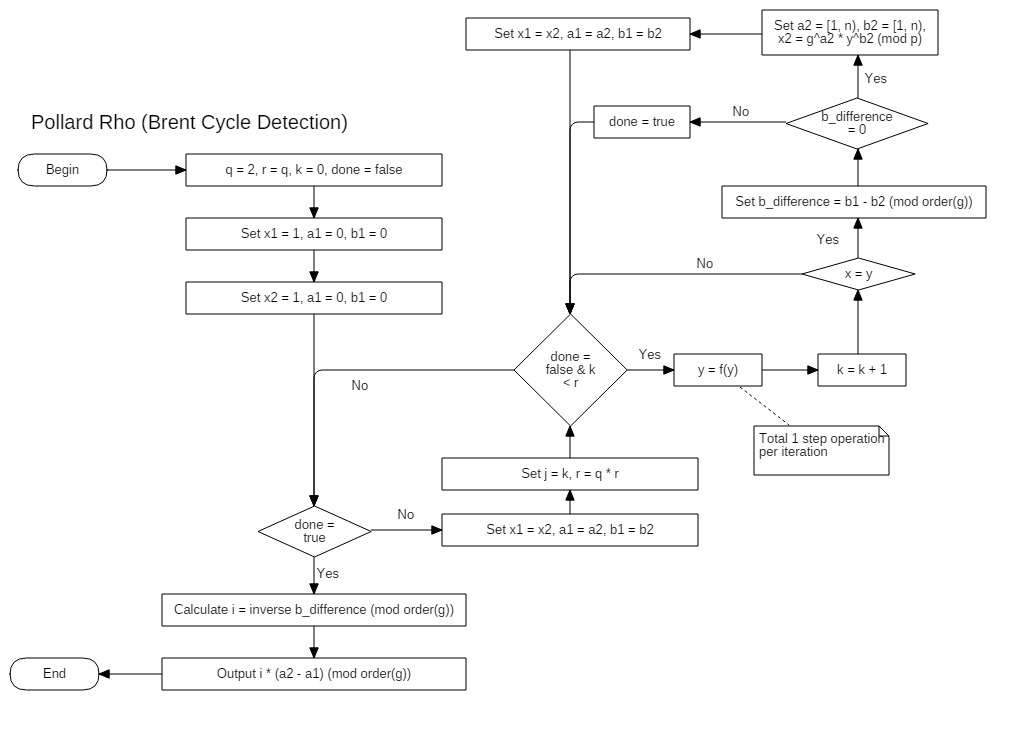
\includegraphics[scale=0.4,angle=90]{bab2/img/pollard-rho-brent}
	\caption {Diagram Alur Metode Deteksi Siklus Brent}
	\label{fig:brent_pollard_rho}
\end{figure}

Cara ini bisa gagal apabila selisih indeks pangkat $ \beta $ bernilai $ 0\ (mod\ n) $. Apabila hal tersebut terjadi, ulangi pencarian nilai $ p_{\text{turtle}} = p_{\text{hare}} $ dari awal, namun kedua \textit{pointer} dimulai dari $ f(x)=\alpha^i \beta^j\ (mod\ n) $, dimana $ 0 \leq i < n $ dan $ 0 \leq j < n $. \textit{Brent Cycle Detection} memiliki kompleksitas sebesar $ O(\sqrt{n}) $.

\section{Strategi Perkalian Modular}

Perkalian modular adalah persamaan \eqref{eq:persamaan_umum_perkalian_modular}.
\begin{equation}
a*b=c\ (mod\ n)
\label{eq:persamaan_umum_perkalian_modular}
\end{equation}

Sebelumnya telah dijelaskan bahwa terdapat kemungkinan terjadinya \textit{integer overflow} karena besarnya nilai $ p $. Maka perlu digunakan sebuah metode perkalian yang dapat menghindari kasus \textit{integer overflow}. Mengingat proses perkalian merupakan proses yang sering terjadi, metode tersebut juga sebaiknya memiliki kecepatan yang tinggi. Pada subbab ini akan dijabarkan dua metode perkalian yang dapat digunakan.

\subsection{Strategi Naif Perkalian Modular}

Strategi naif ini sebenarnya adalah persamaan \eqref{eq:mod_kali} yang ditulis dalam bentuk persamaan \eqref{eq:mod_kali_long}. Hal ini berguna untuk menekan nilai $ a $ dan $ b $ yang tinggi. Setelah dilakukan perkalian, terdapat kemungkinan hasil perkalian melebihi nilai modulus $ n $. Maka dari itu, hasil perkalian $ a $ dan $ b $ kembali dimodulus sekali lagi dengan $ n $. Gambar \ref{psdo:modmul_naive} memaparkan strategi yang dimaksud.

\begin{figure}[h!]
\begin{lstlisting}[firstnumber=0,captionpos=b]
NAIVE-MODULAR-MULTIPLICATION (a, b, n)
return ((a mod n) * (b mod n)) mod n
\end{lstlisting}
\caption{Pseudocode Metode Perkalian Modular Naif}
\label{psdo:modmul_naive}
\end{figure}

Metode ini dapat digunakan untuk $ n \leq 2^{32} $ karena hasil terbesar yang mungkin didapat dari perkalian modular dimana $ n \leq 2^{32} $ adalah $ a*b = c \Rightarrow ( 2^{32}-1 ) * ( 2^{32}-1 ) = 2^{64} - 2^{33} + 1 $. Nilai ini masih dapat ditampung menggunakan 64-bit \textit{integer}.

\subsection{Strategi Perkalian Modular dengan Logarithmic Modular Multiplication} 
Metode \textit{Logarithmic Modular Multiplication} merupakan analog dari \textit{Modular Expontiation} \cite{geeks_modular_multiplication}. Yang membedakan adalah ketimbang pemangkatan, \textit{Logarithmic Modular Multiplication} melakukan perkalian seperti yang ditunjukkan persamaan \eqref{eq:persamaan_umum_perkalian_modular}. Gambar \ref{fig:log_mod_mul} menjelaskan langkah metode ini.

\begin{figure}
	\Centering
	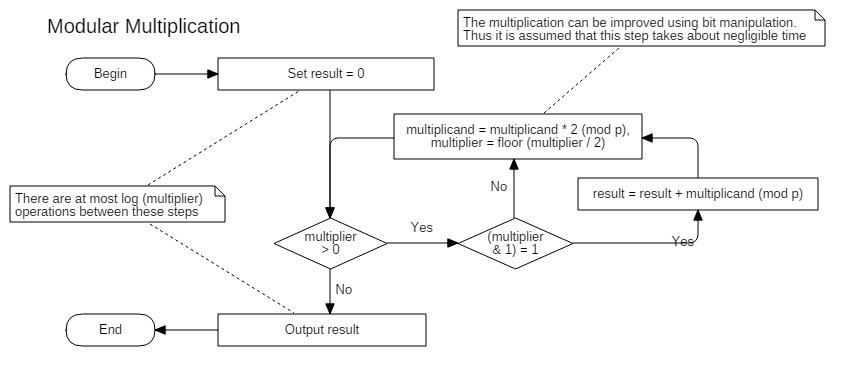
\includegraphics[angle=90,scale=0.5]{bab2/img/modular-multiplication}
	\caption{Diagram Alur \textit{Logarithmic Modular Multiplication}}
	\label{fig:log_mod_mul}
\end{figure}

Strategi ini memiliki kompleksitas $ O(log\ b) $.

\subsection{Penjelasan Strategi Perkalian Modular dengan Logarithmic Modular Multiplication}

Nilai $ b $ pada persamaan \eqref{eq:persamaan_umum_perkalian_modular} pertama-tama diubah menjadi sebuah polinomial \eqref{eq:dekomposisi_biner_perkalian}.
\begin{equation}
b=2^{0}*b_0+2^{1}*b_1+2^{2}*b_2+\ldots+2^{t}*b_t
\label{eq:dekomposisi_biner_perkalian}
\end{equation}
Kemudian kalikan kedua sisi persamaan dengan $ a $.
\begin{align}
ab &= a2^{0}*b_0+a2^{1}*b_1+\ldots+a2^{t}*b_t \\
ab &= \sum_{i=0}^{t} a2^{i}*b_i 
\label{eq:generalisasi_dekomposisi_biner_perkalian}
\end{align}
Maka perhitungan perkalian $ a $ dengan $ b $ merupakan persamaan \eqref{eq:generalisasi_dekomposisi_biner_perkalian}. Nilai $ a $ secara perlahan dikalikan dengan nilai $ 2^{i} $. Metode penghitungan persamaan \eqref{eq:generalisasi_dekomposisi_biner_perkalian} sama dengan cara penghitungan persamaan \eqref{eq:generalisasi_dekomposisi_biner_pemangkatan}. Apabila $ a_i = a * 2^i $, maka dengan memanfaatkan proses perkalian $ 2^i $ yang saling \textit{overlap} (seperti penghitungan $ 2^7 $ pasti membutuhkan hasil penghitungan $ 2^4 $) nilai $ a_i $ dapat ditulis dengan relasi \eqref{eq:relasi_rekurens_a_i}.
\begin{subequations}
	\[
	a_i=
	\begin{cases}
	a, 			& \text{if } i = 0 \\
	a_{i-1} * 2	& \text{if } i > 0
	\end{cases}
	\tag{\ref{eq:relasi_rekurens_a_i}}
	\]
	\label{eq:relasi_rekurens_a_i}
\end{subequations}
Kemudian diberikan sebuah nilai $ term(x)=a_x * b_x $. Maka $ term(x) $ dapat ditulis menjadi persamaan \eqref{eq:relasi_termx}.
\begin{subequations}
\[
	term(x)=
	\begin{cases}
		0, 		& \text{if } b_x=0 \\
		a_i		& \text{if } b_x=1
	\end{cases}
	\tag{\ref{eq:relasi_termx}}
\]
\label{eq:relasi_termx}
\end{subequations}
Sehingga persamaan \eqref{eq:generalisasi_dekomposisi_biner_perkalian} dapat ditulis menjadi persamaan \eqref{eq:generalisasi_dekomposisi_biner_perkalian_rekursif}.
\begin{equation}
	ab = \sum_{i=0}^{t} term(i)
	\label{eq:generalisasi_dekomposisi_biner_perkalian_rekursif}
\end{equation}

Untuk menghitung nilai $ a_i $, kalikan nilai $ a_{i-1} $ yang tersimpan dengan 2. Cara ini dapat digunakan hingga $ a_{(\log b)} $ sehingga penghitungan $ f(n) $ akan membutuhkan $ O(\log b) $ proses perkalian dengan dua. Konsekuensinya, persamaan \eqref{eq:relasi_termx} membutuhkan $ O(\allowbreak\log b) $ proses perkalian. Metode ini dapat digunakan untuk perkalian hingga 63-bit.

\section{Landasan Terkait Pengujian Kebenaran Program}
Keluaran program yang akan digunakan untuk menyelesaikan permasalahan perlu diujikan kebenarannya. Untuk itu perlu dibuat masukan yang mengikuti penjelasan soal seperti yang telah diterangkan pada subbab \ref{sec:Parameter Masukan}. Beberapa teori dan landasan yang akan dimanfaatkan untuk membuat parameter masukan akan dijabarkan pada subbab ini.

\subsection{Miller-Rabin Primality Test}

Subbab ini menjelaskan sebuah metode untuk melakukan pengecekan keprimaan sebuah bilangan, yaitu \textit{Miller-Rabin Primality Test}. Metode ini akan digunakan untuk membangun beberapa parameter.

Metode pengecekan keprimaan \textit{Miller-Rabin} digunakan sebagai alternatif metode pengecekan keprimaan secara naif (dimana metode tersebut memiliki kompleksitas $ O(\sqrt{n})) $. Metode ini menggunakan dasar bahwa apabila terdapat sebuah bilangan ganjil $ n $, kemudian dicari nilai $ s $ dan $ r $ yang memenuhi persamaan $ n-1=2^{s} r $, dan apabila $ n $ merupakan bilangan prima, maka setidaknya salah satu dari kedua persamaan berikut akan bernilai benar. \cite{hac_publickey, stallings_cryptography}
\begin{align}
\label{eq:miller_rabin_condition_1}
a^r &\equiv 1\ (mod\ n), & \gcd(a,n)=1 \\
\label{eq:miller_rabin_condition_2}
a^{2^j r} &\equiv -1\ (mod\ n), & \gcd(a,n)=1,\ 0 \leq j <s-1
\end{align}
Persamaan \eqref{eq:miller_rabin_condition_1} dan \eqref{eq:miller_rabin_condition_2} memberi batasan tersirat $ a>0 $. Untuk seterusnya, nilai $ a $ akan diasumsikan jatuh pada rentang $ 1 \leq a < n $.

Untuk $ n $ yang berupa bilangan prima, salah satu dari persamaan di atas pasti akan terpenuhi. Namun untuk $ n $ yang bukan merupakan bilangan prima, terdapat nilai $ a $ yang memenuhi kedua persamaan di atas. Bilangan $ a $ ini umum disebut dengan \textit{strong liar} terhadap keprimaan $ n $. Artinya, bilangan $ a $ seolah-olah menunjukkan bahwa nilai $ n $ merupakan bilangan prima sebab nilai $ a $ tersebut memenuhi persamaan \eqref{eq:miller_rabin_condition_1} atau \eqref{eq:miller_rabin_condition_2}. Kehadiran \textit{strong liar} untuk $ n $ paling banyak berjumlah $ \frac{1}{4} \phi(n) $ dimana $ \phi(n) $ merupakan \textit{Euler Totient Function}. Artinya kemungkinan nilai komposit $ n $ dianggap sebagai bilangan prima paling besar adalah $ 25\% $. \cite{hac_publickey}

Kemungkinan terjadinya galat pada metode \textit{Miller-Rabin} dapat diperkecil dengan beberapa kali mengecek nilai $ a $ yang berbeda-beda. Untuk $ t $ kali percobaan, kemungkinan terjadinya galat pada metode \textit{Miller-Rabin} adalah paling banyak $ (\frac{1}{4})^{t} $. Semakin besar nilai $ t $, semakin kecil kemungkinan terjadinya galat. \cite{hac_publickey}

\textit{Miller-Rabin} awalnya adalah metode probabilistik untuk menentukan keprimaan sebuah bilangan. Namun dengan membatasi nilai yang akan diperiksa jatuh pada rentang $ 2 \leq n < 2^{64} $, metode \textit{Miller-Rabin} berubah menjadi metode deterministik. Online Encyclopedia of Integer Sequence \cite{oeis_mrabin_limit} menjabarkan sederet nilai yang merupakan nilai batas atas pengujian Miller-Rabin yang tidak akan menghasilkan keluaran yang salah jika diujikan dengan himpunan nilai $ a $ tertentu. Himpunan ini merupakan $ i $ bilangan prima pertama dimana $ i $ adalah suku ke-i pada deretan nilai batas atas. Tabel \ref{tab:miller_rabin_deterministic_a} berisi himpunan yang dimaksud.

\begin{table}[h!]
	\caption{Himpunan Bilangan Pengecek Keprimaan Miller Rabin Jika N Kurang Dari Batas Atas}
	\label{tab:miller_rabin_deterministic_a}
	\ttfamily
	\begin{tabularx}{\linewidth}{ |l|l|X| }
		\hline
		i&	Batas Atas&	\{a\} \\
		\hline
		1&	2047&	2 \\
		2&	1373653&	2, 3 \\
		3&	25326001&	2, 3, 5 \\
		4&	3215031751&	2, 3, 5, 7 \\
		5&	2152302898747&	2, 3, 5, 7, 11 \\
		6&	3474749660383&	2, 3, 5, 7, 11, 13 \\
		7&	341550071728321&	2, 3, 5, 7, 11, 13, 17 \\
		8&	341550071728321&	2, 3, 5, 7, 11, 13, 17, 19 \\
		9&	3825123056546413051&	2, 3, 5, 7, 11, 13, 17, 19, 23 \\
		10&	3825123056546413051&	2, 3, 5, 7, 11, 13, 17, 19, 23, 29 \\
		11&	3825123056546413051&	2, 3, 5, 7, 11, 13, 17, 19, 23, 29, 31 \\
		12&	318665857834031151167461&	2, 3, 5, 7, 11, 13, 17, 19, 23, 29, 31, 37 \\
		\hline
	\end{tabularx}
\end{table}

\subsection{Polinomial Pembuat Bilangan Prima}

Pencarian bilangan prima dapat dilakukan dengan mencoba nilai satu per satu dan mengecek apakah nilai tersebut merupakan bilangan prima atau bukan. Cara ini cenderung tidak efektif. Untuk mempersingkat waktu pencarian bilangan prima, digunakan sebuah polinomial penghasil prima.

Polinomial pembuat bilangan prima yang digunakan adalah polinomial \eqref{eq:polinomial_pembuat_prima}. \cite{wolfram_prime_polynomial}
\begin{equation}
f(n)=n^2+n+41
\label{eq:polinomial_pembuat_prima}
\end{equation}

Walaupun polinomial \eqref{eq:polinomial_pembuat_prima} disebut dengan polinomial penghasil prima, keluaran polinomial ini belum tentu selalu bilangan prima sehingga perlu dilakukan pengecekan keprimaan. Kendati begitu, penggunaan polinomial ini mampu mempercepat pencarian bilangan prima dibandingkan metode naif.
 \cleardoublepage
		\chapter{DESAIN}

Pada bab ini akan dijelaskan desain algoritma yang akan digunakan untuk menyelesaikan permasalahan.

\section{Deskripsi Umum Sistem}

Sistem akan menerima tujuh nilai masukan: $ N $, $ L $, $ q $, $ p $, $ g $, $ y $, $ Hm $. Nilai masukan ini mengikuti penjelasan pada subbab \ref{sec:Parameter Masukan}. Kemudian sistem akan mencari sebuah nilai $ x $ pada persamaan $ y=g^x\ (mod\ p) $. Nilai $ x $ ini akan digunakan pada tahapan pembuatan \textit{signature}, mengacu pada prosedur yang dijabarkan pada subbab \ref{sec:Keluaran Permasalahan}. Seusai pembuatan \textit{signature}, sistem akan mengeluarkan \textit{signature} yang telah dibuat yaitu sepasang nilai \textit{(r, s)}.

Pada tahap penyelesaian logaritma diskret, sistem menggunakan dua metode yang berbeda. Masing-masing metode akan digunakan untuk dibandingkan kinerja satu sama lainnya.

\section{Desain Program Utama}

Subbab ini akan menjelaskan desain fungsi yang akan digunakan untuk menyelesaikan permasalahan.

\subsection {Desain Fungsi Main}

Pada fungsi ini, semua tahapan komputasi berjalan. Termasuk pada tahapan ini yaitu pencarian logaritma diskret dan pembuatan \textit{signature}. Fungsi ini menerima parameter secara interaktif dari pengguna, dan mengeluarkan hasil \textit{signature} \textit{(r, s)} secara interaktif kepada pengguna. Desain fungsi ini dapat dilihat pada gambar \ref{psdo:main}.
\begin{figure}[h!]
\begin{lstlisting}[firstnumber=0]
MAIN
let n, l, q, p, g, y, Hm = Input()
let x = DISCRETE-LOG (q, p, g, y)
let r, s = SIGN (q, p, g, Hm, x)
output (r, s)
\end{lstlisting}
\caption{Desain Fungsi \textit{Main}}
\label{psdo:main}
\end{figure}

\subsection{Desain Fungsi Pencarian Logaritma Diskret}

Terdapat dua metode pencarian logaritma diskret yang akan diujikan pada penyelesaian permasalahan. Subbab ini akan menjelaskan desain masing-masing metode.

\subsubsection {Desain Fungsi Baby-step Giant-step}

Subbab ini akan menjabarkan desain fungsi \textit{Baby-step Giant-step} menurut penjelasan pada subbab \ref{sec:Strategi Penyelesaian Logaritma Diskret dengan Baby-step Giant-step} dalam bentuk \textit{pseudocode}. Fungsi ini menerima tiga \textit{integer}, yaitu $ g $, $ y $, $ n $. Keluaran fungsi ini adalah sebuah \textit{integer} $ x $. Masukan dan keluaran fungsi ini mengacu pada persamaan \eqref{eq:persamaan_umum_log_diskret}. Desain fungsi ini dapat dilihat pada gambar \ref{psdo:bsgs}. Algoritma ini mengikuti penjelasan di \cite{hac_numtheory}.
\begin{figure}[h!]
\begin{lstlisting}[firstnumber=0]
BABY-STEP-GIANT-STEP (g, y, n)
let limit = sqrt (ord(g)) rounded upward
let GIANTSTEPS[] be a new array
let BABYSTEPS[] be a new array
for i = 0 to limit-1
	store pair ~$ \langle s = limit*i, t = g ^ {limit*i} \rangle $~ into GIANTSTEPS
for j = 0 to limit-1
	store pair <s = j, t = y * g^j> into BABYSTEPS
find a match between GIANTSTEPS and BABYSTEPS on the t.
if a pair (x, y) such that said match exist
	return GIANTSTEPS[x].s – BABYSTEPS[y].s
return "NOT FOUND"
\end{lstlisting}
\caption{Desain Fungsi \textit{Baby-step Giant-step}}
\label{psdo:bsgs}
\end{figure}

\subsubsection {Desain Fungsi Pollard Rho dengan Brent Cycle Detection}

Subbab ini akan menjabarkan desain fungsi \textit{Pollard Rho} dengan \textit{Brent Cycle Detection} menurut penjelasan pada subbab \ref{sec:Strategi Penyelesaian Logaritma Diskret dengan Pollard Rho} dan \ref{sec:Brent Cycle Detection}. Fungsi ini menerima tiga \textit{integer}, yaitu $ g $, $ y $, dan $ n $. Keluaran fungsi ini adalah \textit{integer} $ x $. Masukan dan keluaran fungsi ini mengacu pada persamaan \eqref{eq:persamaan_umum_log_diskret}. Desain fungsi ini dapat dilihat pada gambar \ref{psdo:brent_pollard_rho}. Algoritma ini mengikuti penjelasan di \cite{hac_numtheory,brent_montecarlo}.
\begin{figure}[h!]
\begin{lstlisting}[firstnumber=0]
POLLARD-RHO-BRENT (g, y, n)
let p1 = 1, p2 = 1
let i = 2
let iteration = 0
do
	move p1 forward once 
	iteration = iteration + 1
	if iteration == 2^i
		move p2 to p1
		i = i + 1
		iteration = 0
while p1 != p2
let inverse = (p1.b – p2.b)-1 (mod n)
return (p2.a – p1.a) * inverse (mod n)
\end{lstlisting}
\caption{Desain Fungsi \textit{Pollard Rho} dengan \textit{Brent Cycle Detection}}
\label{psdo:brent_pollard_rho}
\end{figure}

\subsubsection {Desain Fungsi Step Untuk Pollard Rho}
Subbab ini akan menjabarkan desain fungsi \textit{Step} pada \textit{Pollard Rho}. Pada subbab \ref{sec:Strategi Penyelesaian Logaritma Diskret dengan Pollard Rho}. dijelaskan bahwa fungsi step butuh mempartisikan himpunan $ \mathbb{Z}_p $ menjadi tiga himpunan. Partisi ini dapat dilakukan dengan mudah dengan melakukan modulus setiap elemen $ \mathbb{Z}_p $ dengan 3, sehingga terbentuk tiga kelas residu: $ [0]_3,[1]_3,[2]_3 $. Ketiga kelas residu ini merepresentasikan tiga himpunan yang digunakan fungsi \textit{}step, dimana $ S_1=[1]_3 $, $ S_2=[0]_3 $, dan $ S_3=[2]_3 $.

Fungsi ini menerima empat \textit{integer} sebagai parameter. Keluaran fungsi ini adalah sebuah \textit{integer} hasil proses \textit{step}. Desain fungsi ini dapat dilihat pada gambar \ref{psdo:step}.
\begin{figure}[h!]
\begin{lstlisting}[firstnumber=0]
STEP (value, alpha, beta, modulus)
let class = value mod 3
if class == 0
	value = MODULAR-MULTIPLICATION (value, value, modulus)
else if class == 1
	value = MODULAR-MULTIPLICATION (value, beta, modulus)
else
	value = MODULAR-MULTIPLICATION (value, alpha, modulus)
return value
\end{lstlisting}
\caption{Desain Fungsi \textit{Step}}
\label{psdo:step}
\end{figure}

\subsection{Desain Fungsi Sign}

Subbab ini akan menjabarkan desain fungsi Sign yang mengikuti prosedur pada subbab \ref{sec:Keluaran Permasalahan}. Fungsi ini menerima lima \textit{integer} sebagai parameter dan dua \textit{integer} sebagai keluaran. Desain fungsi ini dapat dilihat pada gambar \ref{psdo:sign}.
\begin{figure}[h!]
\begin{lstlisting}[firstnumber=0]
SIGN (globalMod, keyMod, g, hash, x)
let i = 1
let r, s = 0, 0

while r == 0 do
	i = i + 1
	r = MODULAR-EXPONENTIATION (g, i, keyMod, globalMod)
	if r != 0
		let inverse = MODULAR-INVERSE (generator, keyMod)
		s = (hash + r * x) mod q
		s = (s * inverse) mod q
		if s != 0
			return (r, s)
	r = 0
\end{lstlisting}
\caption{Desain Fungsi \textit{Sign}}
\label{psdo:sign}
\end{figure}

\subsection{Desain Fungsi Modular Exponentiation}

Subbab ini akan menjabarkan desain fungsi \textit{Modular Exponentiation}, mengacu pada penjelasan pada subbab \ref{sec:Strategi Penyelesaian Pemangkatan Modular dengan Repeated Squaring}. Fungsi ini menghitung $ g^k\ mod\ p $, dimana $ g $ memiliki order elemen $ q $. Fungsi ini menerima empat \textit{integer} sebagai input dan mengeluarkan sebuah \textit{integer} sebagai hasil penghitungan pemangkatan modular. Desain fungsi ini dapat dilihat pada gambar \ref{psdo:modex}.
\begin{figure}[h!]
\begin{lstlisting}[firstnumber=0]
MODULAR-EXPONENTIATION (g, k, p, q)
let result = 1
let basis = 1
k = k mod q
let ~$ \left\langle k_0,\ k_1,\ \dots,\ k_n\right\rangle $~ be a bit representation of k where ki is the ith bit.
for i = 1 to n
	basis = (basis * g) mod p
		if ~$ k_i $~ == 1
		result = (result * basis) mod p
return result
\end{lstlisting}
\caption{Desain Fungsi \textit{Modular Exponentiation}}
\label{psdo:modex}
\end{figure}

\subsection{Desain Fungsi Logarithmic Modular Multiplication}

Subbab ini akan menjabarkan desain fungsi \textit{Logarithmic Modular Multiplication} mengikuti penjelasan pada subbab \ref{sec:Strategi Perkalian Modular dengan Logarithmic Modular Multiplication}. Fungsi ini menerima tiga masukan: sebuah nilai yang dikali $ a $, sebuah nilai pengali $ b $, dan sebuah modulus $ n $. Keluaran fungsi ini adalah sebuah \textit{integer} hasil perkalian. Desain fungsi ini dapat dilihat pada gambar \ref{psdo:modmul}. Algoritma ini mengikuti penjelasan di \cite{geeks_modular_multiplication}.
\begin{figure}[h!]
\begin{lstlisting}[firstnumber=0]
LOGARITHMIC-MODULAR-MULTIPLICATION (a, b, n)
let result = 1, basis = a
let ~$ \left\langle b_1,\ b_2,\ \dots ,\ b_t \right\rangle $~ be the i-th bit representation for b
for i = 1 to t
	if ~$ b_i $~ == 1
		result = (result + basis) mod n
	basis = (basis * 2) mod n
return result
\end{lstlisting}
\caption{Desain Fungsi Modular Multiplication}
\label{psdo:modmul}
\end{figure}

\subsection{Desain Fungsi Invers Modulus}

Fungsi ini digunakan pada banyak bagian penyelesaian permasalahan. Cara kerja fungsi ini mengacu pada penjelasan di subbab \ref{sec:Strategi Penyelesaian Invers Modulus dengan Extended Euclidean}. Fungsi menerima sebuah persamaan \ref{eq:persamaan_umum_pembagian}. Keluaran metode ini adalah koefisien sebuah nilai $ a $ dan sebuah modulus $ b $. Desain fungsi ini dapat dilihat pada gambar \ref{psdo:modinv}. Algoritma ini didapat dari \cite{hac_math}.
\begin{figure}[h!]
\begin{lstlisting}[firstnumber=0]
MODULAR-INVERSE (a = qb + r)
let EQUATION[] be a new array
let i = 0
while r != 0
	EQUATION[i] = (a = qb + r)
	find equation b = qr + m for some q and m
	i = i + 1
for i = EQUATION.len – 2 downto 0
	substitute EQUATION[i].b with EQUATION[i+1].r
return (EQUATION[0].a.coefficient, EQUATION[0].b.coefficient)
\end{lstlisting}
\caption{Desain Fungsi Invers Modulus}
\label{psdo:modinv}
\end{figure}

\subsection{Desain Fungsi Uji Kebenaran}

Fungsi uji kebenaran digunakan untuk melakukan uji coba kebenaran keseluruhan program pada tahapan komputasi utama. Fungsi ini akan digunakan sebagai \textit{catch-all error detection} untuk membantu proses \textit{debugging}. Fungsi ini bekerja mengikuti prosedur pada subbab \ref{sec:Lain-lain}.

Fungsi ini menerima tujuh \textit{integer} sebagai masukan dimana lima pertama merupakan masukan soal, dan dua selanjutnya merupakan \textit{signature} yang dibuat. Keluaran fungsi ini adalah enumerasi benar\textendash salah. Desain fungsi ini dapat dilihat pada gambar \ref{psdo:verify}.
\begin{figure}[h!]
\begin{lstlisting}[firstnumber=0]
VERIFY (q, p, g, y, Hm, r, s)
let w = MODULAR-INVERSE (s, q)
let u1 = MODULAR-MULTIPLICATION (w, Hm, q)
let u2 = MODULAR-MULTIPLICATION (w, r, q)
let g' = MODULAR-EXPONENTIATION (g, u1, p, p-1)
let y' = MODULAR-EXPONENTIATION (y, u2, p, p-1)
let v = MODULAR-MULTIPLICATION (g’, y’, q)
if v == r
	return "SIGNATURE CORRECT"
return "SIGNATURE INCORRECT"
\end{lstlisting}
\caption{Desain Fungsi Uji Kebenaran}
\label{psdo:verify}
\end{figure}

\section{Desain Program Pembuat Data Uji}

Program tahapan komputasi utama memiliki masukan yang tidak sembarangan. Masukan program memiliki sifat-sifat yang dijelaskan pada subbab \ref{sec:Parameter Masukan}. Program ini membentuk data uji untuk membantu memeriksa kebenaran program utama.

\subsection{Desain Fungsi Main Program Pembuat Data Uji}

Semua hal yang berkaitan dengan pembuatan data uji berjalan pada fungsi ini. Desain fungsi ini dapat dilihat pada gambar \ref{psdo:main_generator}.

\begin{figure}[h!]
\begin{lstlisting}[firstnumber=0]
MAIN
let begin = Input()
let end = Input()
let bitDifference = Input()
let limit = Input()
let Hm = Input()
for i = begin to end
	GENERATE (i, i + bitDifference, Hm, limit)
\end{lstlisting}
\caption{Desain Fungsi Utama Pembuat Data Uji}
\label{psdo:main_generator}
\end{figure}

\subsection{Desain Fungsi Pengecekan Keprimaan}

Subbab ini akan menjelaskan metode pengecekan keprimaan berdasarkan penjelasan pada subbab \ref{sec:Miller-Rabin Primality Test}. Masukan fungsi ini adalah sebuah bilangan \textit{integer}. Keluaran fungsi ini adalah enumerasi prima\textendash komposit. Desain fungsi ini dapat dilihat pada gambar \ref{psdo:miller_rabin}.
\begin{figure}[h!]
\begin{lstlisting}[firstnumber=0]
IS-PRIME (value)
if value == 2
	return "PRIME"
if value < 2 or value is divisible with 2
	return "COMPOSITE"
let s = 0
let r = value – 1
while r is divisible with 2
	s = s + 1
	r = r / 2
let PRIMES be array of 12 first primes
let LIMITS be array of 12 Miller-Rabin upper limits
let limit = first index where value < LIMITS[index]
for i = 0 to limit - 1
	let m = MODULAR-EXPONENTIATION (value, a[i], r, r-1)
	if y != 1 or y != (value – 1)
		let j = 1
		while j < s-1 and y != (value – 1)
			y = (y * y) mod value
			if y == 1
				return "PRIME"
			j = j + 1
		if y != (value – 1)
			return "COMPOSITE"
return "PRIME"
\end{lstlisting}
\caption{Desain Fungsi Pengecekan Keprimaan Miller Rabin}
\label{psdo:miller_rabin}
\end{figure}

\subsection{Desain Fungsi Polinomial Prima}

Fungsi ini mengevaluasi polinomial pada persamaan \eqref{eq:polinomial_pembuat_prima} pada subbab \ref{sec:Polinomial Pembuat Bilangan Prima} untuk membentuk bilangan prima. Fungsi ini menerima sebuah \textit{integer} sebagai masukan, dan mengeluarkan \textit{integer} sebagai keluaran. Desain fungsi ini dapat dilihat pada gambar \ref{psdo:prime_generator_polynomial}.
\begin{figure}[h!]
\begin{lstlisting}[firstnumber=0]
POLY-PRIME (n)
return n*n + n + 41
\end{lstlisting}
\caption{Desain Fungsi Polinomial Pembuat Bilangan Prima}
\label{psdo:prime_generator_polynomial}
\end{figure}

\subsection{Desain Fungsi Generate}

Fungsi ini bertujuan untuk membuat data uji dengan karakteristik masukan yang diberikan. Dalam satu pemanggilan fungsi, akan dibuatkan paling banyak sebanyak \textit{limit} data uji yang memenuhi karakteristik masukan. Fungsi ini menerima empat \textit{integer} sebagai masukan, dan delapan \textit{integer} sebagai keluaran. Tujuh dari delapan \textit{integer} pertama merupakan nilai masukan soal mengikuti penjelasan di subbab \ref{sec:Parameter Masukan}. Desain fungsi ini dapat dilihat pada gambar \ref{psdo:generate}.
\begin{figure}[h!]
\begin{lstlisting}[firstnumber=0]
GENERATE (N, L, Hm, limit)
let NLimit be the highest N-bit value possible
let LLimit be the highest L-bit value possible
let NBegin be the highest (N-1)-bit value possible
let LBegin be the highest (L-1)-bit value possible
let q = 0
let i = sqrt (NBegin)
while q < NLimit
	q = POLY-PRIME (i)
	i = i + 1
	if IS-PRIME (q) == "COMPOSITE" or q < NBegin
		continue
	for p = LBegin + q – (LBegin mod q) to LLimit
		if IS-PRIME (p) == "COMPOSITE" or p is not divisible with q
			continue
		let g = 1
		for k = 2 to q-1
		find a value of g = k^(p/q) mod (p+1) that doesn’t result in 1 and g^q mod (p+1) results in 1
		if such g found
			let x a random value between 1 and q-1 inclusive
			let y = MODULAR-EXPONENTIATION (g, x, j + 1, j)
			output (N, L, q, j + 1, g, y, Hm, x)
			limit = limit - 1
			if limit == 0
				quit function
\end{lstlisting}
\caption{Desain Fungsi \textit{Generate}}
\label{psdo:generate}
\end{figure} \cleardoublepage
		\chapter {IMPLEMENTASI}

\section{Lingkungan implementasi}

Lingkungan implementasi dan pengembangan yang dilakukan adalah sebagai berikut.
\begin{enumerate}
	\item Perangkat Keras
	\begin{enumerate}
		\item Processor Intel® Core™ i5-7400 CPU @ 3.00GHz (4 CPUs), ~3.0GHz
		\item Random Access Memory 8192MB
	\end{enumerate}
	\item Perangkat Lunak
	\begin{enumerate}
		\item Sistem Operasi Windows 10 Pro 64-bit
		\item IDE CodeBlocks 17.12
		\item Bahasa Pemrograman C++
		\item MinGW 64-bit
	\end{enumerate}
\end{enumerate}

\section{Implementasi Program Utama}

Subbab ini menjelaskan implementasi program utama. Program ini merupakan program yang digunakan untuk menyelesaikan permasalahan DSA Attack.

\subsection{Penggunaan Library, Tipe data, dan Struct}

Program ini menggunakan beberapa \textit{library} dan tipe data seperti yang ditunjukkan pada kode sumber \ref{code:header_main}.

\begin{code}[firstnumber=1,float]{\textit{Header} Program Utama}{header_main}
#include <cstdio>
#include <cstdlib>
#include <unordered_map>
#include <utility>
#include <cmath>
#include <vector>

typedef unsigned long long uint64;
typedef          long long int64;
\end{code}

Untuk mengakomodasi aritmatika modular, sebuah \textit{struct} dengan tujuan tersebut diimplementasikan. Kode sumber \ref{code:zelement_1} sampai \ref{code:zelement_5} menjelaskan implementasi \textit{struct} yang dimaksud.

\newpage

\begin{code}[firstnumber=0]{\protect\textit{Struct} ZElement (bg. 1)}{zelement_1}
ZElement
uint64 character;
uint64 element;
uint64 order;

ZElement (uint64 character, uint64 element, uint64 order = 0)
{
	this->character = character;
	this->element = element % character;
	this->order = (order == 0) ? character - 1 : order; // Assumes the element is primitive element
}

ZElement (const ZElement & other)
{
\end{code}
\pagebreak
\begin{code}[firstnumber=last]{\textit{Struct} ZElement (bg. 2)}{zelement_2}
	this->character = other.character;
	this->element = other.element;
	this->order = other.order;
}

ZElement ()
{   character = 0; element = 0; order = 0; }

ZElement & operator = (const uint64 & other)
{
	this->element = other % character;
	return *this;
}

ZElement operator + (const uint64 & other)
{
	uint64 output = (element + (other % character)) % character;
	return ZElement (character, output);
}

// TODO: may fail when other >= 2 * character
ZElement operator - (const uint64 & other)
{
	uint64 output = (element >= other) ?
	element - other :
	element - other + character;
	return ZElement (character, output);
}

ZElement operator * (const uint64 & other)
{
	return ZElement (character, modularMultiplication (element, other, character));
\end{code}
\pagebreak
\begin{code}[firstnumber=last]{\textit{Struct} ZElement (bg. 3)}{zelement_3}
}

ZElement operator + (const ZElement & other)
{
	return *this + other.element;
}

ZElement operator - (const ZElement & other)
{
	return *this - other.element;
}

ZElement operator * (const ZElement & other)
{
	return *this * other.element;
}

ZElement & operator += (const uint64 & other)
{
	this->element = (element + (other % character)) % character;
	return *this;
}

// TODO: may fail when other >= 2 * character
ZElement & operator -= (const uint64 & other)
{
	this->element = (element >= other) ?
	element - other :
	element - other + character;
	return *this;
}

ZElement & operator *= (const uint64 & other)
{
\end{code}
\pagebreak
\begin{code}[firstnumber=last]{\textit{Struct} ZElement (bg. 4)}{zelement_4}
	ZElement result = ZElement (character, modularMultiplication (element, other, character));
	this->element = result.element;
	return *this;
}

ZElement & operator += (const ZElement & other)
{
	*this += other.element;
	return *this;
}

// TODO: may fail when other >= 2 * character
ZElement & operator -= (const ZElement & other)
{
	*this -= other.element;
	return *this;
}

ZElement & operator *= (const ZElement & other)
{
	*this *= other.element;
	return *this;
}

bool operator < (const ZElement & other) const
{
	return element < other.element;
}

bool operator == (const ZElement & other) const
{
	return element == other.element;
}
\end{code}
\pagebreak
\begin{code}[firstnumber=last]{\textit{Struct} ZElement (bg. 5)}{zelement_5}
	
bool operator != (const ZElement & other) const
{
	return element != other.element;
}

ZElement invert ()
{
	return ZElement (character, modularInverse (element, character));
}
\end{code}

\subsection{Implementasi Fungsi Main}

Subbab ini menjabarkan implementasi fungsi \textit{main} yang dijelaskan pada subbab~\ref{sec:Desain Fungsi Main}. Implementasi fungsi ini dapat dilihat pada kode sumber \ref{code:main}.

\begin{code}[firstnumber=0]{Fungsi Main}{main}
int main()
uint64  N, // Number of bit for q
L, // Number of bit for p
q, // Global basis
p, // Public key modulus
g, // Generator
y, // Public key query i.e. moduled generator
M; // Hashed message

scanf ("%llu%llu%llu%llu%llu%llu%llu", &N, &L, &q, &p, &g, &y, &M);
uint64 index = BSGS (g, p, y, q);

auto signedPair = sign (M, q, g, p, index);

printf ("%llu %llu\n", signedPair.first.element, signedPair.second.element);
\end{code}

\subsection{Implementasi Fungsi Baby-step Giant-step}

Subbab ini menjabarkan implementasi fungsi \textit{Baby-step Giant-step} yang dijelaskan pada subbab \ref{sec:Desain Fungsi Baby-step Giant-step}. Implementasi fungsi ini dapat dilihat pada kode sumber \ref{code:bsgs_1} sampai \ref{code:bsgs_2}.

\begin{code}[firstnumber=0]{Fungsi \textit{Baby-step Giant-step} (bg. 1)}{bsgs_1}
uint64 BSGS (const uint64 & generator, const uint64 & modulo, const uint64 & query, const uint64 & order)
typedef ZElement key_t;   // Will contain g^(limit * i) mod p
typedef ZElement value_t; // Will contain limit * i mod q

std::unordered_map <key_t, value_t, ZElement_hash> giantStep;

uint64 limit = std::ceil (std::pow (order, 0.5));

ZElement giantStepSize = modularExponentiation (ZElement (modulo, generator, order), limit);
key_t   currentGiantStepKey (modulo, 1);
value_t currentGiantStepValue (order, 0);

for (uint64 i = 0; i <= limit; i++)
{
	giantStep[ currentGiantStepKey ] = currentGiantStepValue;
	currentGiantStepKey *= giantStepSize;
	currentGiantStepValue += limit;
}

key_t poweredResult (modulo, query);
for (uint64 i = 0; i < limit; i++)
{
\end{code}
\pagebreak
\begin{code}[firstnumber=last]{Fungsi \textit{Baby-step Giant-step} (bg. 2)}{bsgs_2}
	auto it = giantStep.find ( poweredResult );
	if (it != giantStep.end())
	return (it->second - i).element;
	poweredResult *= generator;
}

return -1;
\end{code}

Fungsi ini menggunakan \textit{library} \texttt{unordered\textunderscore map}. Untuk itu, dibutuhkan sebuah fungsi untuk menghasilkan \textit{hash value} dari tipe data \texttt{ZElement}. Fungsi tersebut dapat dilihat pada kode sumber \ref{code:zelement_hash}.

\begin{code}[firstnumber=0]{Penghitung Nilai \textit{Hash} Tipe Data ZElement}{zelement_hash}
struct ZElement_hash
size_t operator () (const ZElement & in) const
{
	return  std::hash <uint64> () (in.character) ^
	std::hash <uint64> () (in.element) ^
	std::hash <uint64> () (in.order);
}
\end{code}

\subsection{Implementasi Fungsi Pollard Rho}

Subbab ini akan menjelaskan bagaimana desain fungsi \textit{Pollard Rho} akan diimplementasikan. Fungsi ini merupakan sebuah modul yang komponennya sangat berkaitan. Untuk itu, segala hal yang berkaitan dengan \textit{Pollard Rho} dikumpulkan dalam sebuah \textit{struct} pada kode sumber \ref{code:general_pollard_rho}.

\begin{code}[firstnumber=0, float=h!]{Struktur \textit{Struct Pollard Rho}}{general_pollard_rho}
struct pollardRho
/// variable
// ...
// ...

/// static functions
// ...
// ...
\end{code}

\subsubsection{Penggunaan Struct Step}

Sebuah \textit{struct} untuk akan digunakan untuk melakukan proses \textit{step}. Selain itu, \textit{struct} ini juga berfungsi untuk menyimpan histori \textit{step} setiap \textit{pointer}. \textit{Struct} ini merupakan implementasi desain pada subbab \ref{sec:Desain Fungsi Step Untuk Pollard Rho}. Implementasi \textit{struct} ini dapat dilihat pada kode sumber \ref{code:step_1} dan \ref{code:step_2}.

\begin{code}[firstnumber=0, float]{Struct \textit{Step} (bg. 1)}{step_1}
struct step
ZElement value;
ZElement alpha;
ZElement beta;

step (ZElement value, ZElement alpha, ZElement beta)
{
	this->value = value;
	this->alpha = alpha;
	this->beta = beta;
}

step ()
{
	this->value = ZElement (1, 0);
	this->alpha = ZElement (1, 0);
	this->beta = ZElement (1, 0);
}

void stepPartitionOne (const uint64 & betaValue)
{
	beta += 1;
	value *= betaValue;
}

void stepPartitionTwo ()
{
	alpha += alpha;
	beta += beta;
	value *= value;
}
\end{code}
\begin{code}[firstnumber=last, float=h]{Struct \textit{Step} (bg. 2)}{step_2}
void stepPartitionThree (const uint64 & alphaValue)
{
	alpha += 1;
	value *= alphaValue;
}

/**
*  Defines the step function
*  S1 consists of residue class [1]
*  S2 consists of residue class [0]
*  S3 consists of residue class [2]
*/
step & goForward (const uint64 & A, const uint64 & B)
{
	int residue = value.element & 3;
	if      (residue == 1) stepPartitionOne(B);
	else if (residue == 0) stepPartitionTwo();
	else                   stepPartitionThree(A);
	
	return *this;
}
\end{code}

\textit{Struct} ini memiliki tiga variabel yang penting dalam melakukan proses \textit{step}. Nilai ini tertera pada tabel \ref{tab:var_step}. Nilai A dan B akan ditentukan mengikuti penjelasan pada subbab \ref{sec:Strategi Penyelesaian Logaritma Diskret dengan Pollard Rho}.

\begin{table}[h!]
\caption{Variabel Struct Step}
\label{tab:var_step}
\begin{tabularx}{\linewidth}{ |c|c|X| }
\hline
No	&Nama	&Deskripsi \\
\hline
1	&\textit{value}	&Menyimpan nilai $ v=A^{\alpha} B^{\beta}\ (mod\ m) $ \\
2	&\textit{alpha}	&Menyimpan berapa kali step ini telah dikalikan dengan A \\
3	&\textit{beta}	&Menyimpan berapa kali step ini telah dikalikan dengan B \\
\hline
\end{tabularx}
\end{table}

\subsubsection{Implementasi Fungsi Pollard Rho dengan Brent Cycle Detection}

Subbab ini menjabarkan implementasi fungsi \textit{Pollard Rho} dengan \textit{Brent Cycle Detection} yang dijelaskan pada subbab \ref{sec:Desain Fungsi Pollard Rho dengan Brent Cycle Detection}. Implementasi fungsi ini dapat dapat dilihat pada kode sumber \ref{code:brent_1} dan \ref{code:brent_2}.
\begin{code}[firstnumber=0]{Fungsi \textit{Pollard Rho} dengan \textit{Brent Cycle Detection} (bg. 1)}{brent_1}
static uint64 brent (const uint64 & generator, const uint64 & modulo, const uint64 & query, const uint64 & order)
uint64 nextCheckpoint = 1;
uint64 currentIteration = 0;

step lastCheckpointStep;
step currentStep (ZElement (modulo, 1), ZElement (order, 0), ZElement (order, 0));
\end{code}
\begin{code}[firstnumber=last]{Fungsi \textit{Pollard Rho} dengan \textit{Brent Cycle Detection} (bg. 2)}{brent_2}
ZElement betaDifference;

bool done = false;

while ( ! done )
{
	lastCheckpointStep = currentStep;
	nextCheckpoint = nextCheckpoint * 2;
	
	for (; ( !done ) && currentIteration < nextCheckpoint; currentIteration++)
	{
		currentStep.goForward(generator, query);
		if (currentStep.value == lastCheckpointStep.value)
		{
			betaDifference = lastCheckpointStep.beta - currentStep.beta;

			if (betaDifference.element == 0)
			{
				currentStep = randomizeStartingStep (generator, order, modulo, query);
			}
			else
			{
				done = true;
			}
		}
	}
}

ZElement result = betaDifference.invert();
result *= (currentStep.alpha - lastCheckpointStep.alpha);

return result.element;
\end{code}

\subsubsection{Implementasi Fungsi Pengacakan Posisi Awal}

Subbab ini menjabarkan implementasi fungsi pengacakan posisi awal yang akan digunakan apabila terjadi kasus yang menyebabkan metode \textit{Pollard Rho} gagal memberikan keluaran yang benar seperti yang dijelaskan pada subbab \ref{sec:Brent Cycle Detection}. Implemetasi fungsi ini dapat dilihat pada kode sumber \ref{code:randomize_step}
\begin{code}[firstnumber=0]{Fungsi Pengacakan Posisi Awal}{randomize_step}
static step randomizeStartingStep (const uint64 & generator, const uint64 & order, const uint64 & modulo, const uint64 & query)
uint64 upperLimit = order - 1;
ZElement alpha (order, 1 + (rand() % upperLimit));
ZElement beta (order, 1 + (rand() % upperLimit));

ZElement poweredAlpha = modularExponentiation (ZElement (modulo, generator, order), alpha.element);
ZElement poweredBeta = modularExponentiation (ZElement (modulo, query, order), beta.element);

ZElement value = poweredAlpha * poweredBeta;

return step (value, alpha, beta);
\end{code}

\subsection{Implementasi Fungsi Pemangkatan Modular}

Subbab ini menjabarkan implementasi fungsi pemangkatan modular yang dijelaskan pada subbab \ref{sec:Desain Fungsi Modular Exponentiation}. Implementasi fungsi ini dapat dilihat pada kode sumber \ref{code:modex}.
\begin{code}[firstnumber=0, float=h!]{Fungsi Pemangkatan Modular}{modex}
ZElement modularExponentiation (ZElement generator, uint64 exponent)
ZElement result (generator.character, 1);
if (exponent >= generator.order)
exponent = exponent % generator.order;

for (; exponent > 0; exponent = exponent >> 1)
{
	if (exponent & 1 == 1)
	{
		result = result * generator;
	}
	
	generator = generator * generator;
}

return result;
\end{code}

\subsection{Implementasi Fungsi Perkalian Modular dengan Logarithmic Modular Multiplication}

Subbab ini menjabarkan implementasi fungsi \textit{Logarithmic Modular Multiplication} yang dijelaskan pada subbab \ref{sec:Desain Fungsi Logarithmic Modular Multiplication}. Implementasi fungsi ini dapat dilihat pada kode sumber \ref{code:modmul}.
\begin{code}[firstnumber=0, float=h!]{Fungsi \textit{Logarithmic Modular Multiplication}}{modmul}
uint64 modularMultiplication (uint64 multiplier, uint64 multiplicand, uint64 modulo)
multiplier = multiplier % modulo;
multiplicand = multiplicand % modulo;

if ( multiplier < multiplicand )
std::swap (multiplier, multiplicand);

uint64 result = 0;

while (multiplier > 0)
{
	if ( multiplier & 1 == 1 )
	{
		result = (result + multiplicand) % modulo;
	}
	
	multiplier >>= 1;
	multiplicand = (multiplicand << 1) % modulo;
}

return result;
\end{code}

Untuk mempercepat kinerja fungsi, \textit{sentinel} perulangan yang digunakan adalah nilai terkecil antara \textit{multiplier} dan \textit{multiplicand}.

\subsection{Implementasi Fungsi Invers Modulus}

Subbab ini menjabarkan implementasi fungsi invers modulus yang dijelaskan pada subbab \ref{sec:Desain Fungsi Invers Modulus}. Implementasi fungsi ini dapat dilihat pada kode sumber \ref{code:modinv}.
\begin{code}[firstnumber=0, float=h!]{Fungsi Invers Modulus}{modinv}
uint64 modularInverse (uint64 value, uint64 modulus)
int64 valueCoeff, modulusCoeff;
extendedEuclidean (modulus, value % modulus, modulusCoeff, valueCoeff);

return (valueCoeff < 0) ? valueCoeff + (int64) modulus : valueCoeff;
\end{code}

\subsection{Implementasi Fungsi Sign}

Subbab ini menjabarkan implementasi fungsi \textit{Sign} yang dijelaskan pada subbab \ref{sec:Desain Fungsi Sign}. Implementasi fungsi ini dapat dilihat pada kode sumber \ref{code:sign}.
\begin{code}[firstnumber=0, float]{Fungsi \textit{Sign}}{sign}
std::pair <ZElement, ZElement> sign (const uint64 & message, const uint64 & globalModulo, const uint64 & generator, const uint64 & keyModulo, const uint64 & index) 
std::pair <ZElement, ZElement> output ((ZElement) {globalModulo, 0}, (ZElement) {globalModulo, 0});

ZElement temporalKeypair (globalModulo, 1);
do
{
	temporalKeypair += 1;
	
	output.first = modularExponentiation (ZElement (keyModulo, generator, globalModulo), temporalKeypair.element);
	output.first = ZElement (globalModulo, output.first.element);
	
	if (output.first.element == 0)
	{
		continue;
	}
	
	ZElement inverseTemporalKeypair = temporalKeypair.invert();
	ZElement transformedMessage = ZElement (globalModulo, message + (output.first * index).element);
	
	output.second = inverseTemporalKeypair * transformedMessage;
	
	if (output.second.element == 0)
	{
		output.first.element = 0;
		continue;
	}
} while (output.first.element == 0);

return output;
\end{code}

\subsection{Implementasi Fungsi Uji Kebenaran}

Subbab ini menjabarkan implementasi fungsi uji kebenaran yang dijelaskan pada subbab \ref{sec:Desain Fungsi Uji Kebenaran}. Implementasi fungsi ini dapat dilihat pada kode sumber \ref{code:verify}.
\begin{code}[firstnumber=0]{Fungsi Uji Kebenaran}{verify}
bool verify (const uint64 & globalModulo, const uint64 & keyModulo, const uint64 & generator, const uint64 & query, const uint64 & message, std::pair <ZElement, ZElement> signature)
ZElement w = signature.second.invert();
ZElement u1 = w * message;
ZElement u2 = w * signature.first;
ZElement poweredG = modularExponentiation (ZElement (keyModulo, generator, keyModulo - 1), u1.element);
ZElement poweredY = modularExponentiation (ZElement (keyModulo, query, keyModulo - 1), u2.element);
ZElement v (globalModulo, (poweredG * poweredY).element);
return v.element == signature.first.element;
\end{code}

\section{Implementasi Program Pembuat Data Uji}

Subbab ini akan menjelaskan mengenai implementasi program pembuatan data uji, mengikuti penjelasan pada subbab \ref{sec:Desain Program Pembuat Data Uji}.

\subsection{Penggunaan Library, Konstanta, dan Struct}

Program ini menggunakan \textit{library} bawaan C++, yaitu \texttt{cstdio} yang digunakan untuk menerima dan mengeluarkan hasil luaran program, \texttt{cstdlib} yang digunakan untuk melakukan randomisasi, \texttt{ctime} sebagai \textit{library} untuk melakukan \textit{random seeding}, dan \texttt{utility} yang digunakan untuk melakukan penukaran dua variabel. Selain \textit{library}, sebuah tipe data \textit{unsigned integer} 64-bit juga didefinisikan dengan nama \texttt{uint64}. Keseluruhan penggunaan \textit{library} dan konstanta dapat dilihat pada kode sumber \ref{code:header_generator}.
\begin{code}[firstnumber=1]{\textit{Header} Program Pembuat Data Uji}{header_generator}
#include <cstdio>
#include <cstdlib>
#include <ctime>
#include <utility>

#define uint64 unsigned long long
\end{code}

\subsection{Implementasi Fungsi Main}

Fungsi ini merupakan inti seluruh program. Fungsi ini tidak menerima masukan. Masukan akan diberikan secara \textit{hard-coded}. Masukan tersebut diantaranya adalah nilai $ N $ , nilai $ L $, dan banyaknya pasangan data menurut masukan $ N $ dan $ L $. Pada kode sumber berikut ini, nilai $ N $ adalah 7, nilai $ L $ adalah 10 hingga 60, dan banyaknya pasangan data menurut masukan $ N $ dan $ L $ adalah 7. Kode sumber yang dimaksud dapat dilihat pada kode sumber \ref{code:main_generator}
\begin{code}[firstnumber=0]{Fungsi \textit{Main} Program Pembuat Data Uji}{main_generator}
int main()
srand (time(NULL));
for (int i = 10; i <= 60; i++)
{
	printf ("[N = %d, L = %d]\n", 7, i);
	generateKeypair(7, i, 7);
}

return 0;
\end{code}

\subsection{Implementasi Fungsi Perkalian Modular}

Fungsi ini merupakan implementasi desain fungsi \textit{Logarithmic Modular Multiplication} pada subbab \ref{sec:Desain Fungsi Logarithmic Modular Multiplication}. Implementasi fungsi ini dapat dilihat pada kode sumber \ref{code:modmul_generator}
\begin{code}[firstnumber=0]{Fungsi \textit{Logarithmic Modular Multiplication}}{modmul_generator}
uint64 modularMultiplication (const uint64 & cMultiplicand, const uint64 & cMultiplier, const uint64 & modulus)
uint64 multiplicand = cMultiplicand % modulus;
uint64 multiplier = cMultiplier % modulus;

if ( multiplier < multiplicand )
std::swap (multiplier, multiplicand);

uint64 result = 0;

while ( multiplier > 0 )
{
	if ( multiplier & 1 == 1 )
	{
		result = (result + (multiplicand % modulus)) % modulus;
	}
	
	multiplier >>= 1;
	multiplicand = (multiplicand << 1) % modulus;
}

return result;
\end{code}

\subsection{Implementasi Fungsi Pemangkatan Modular}

Fungsi ini merupakan implementasi desain pada subbab \ref{sec:Desain Fungsi Modular Exponentiation}. Terdapat sedikit penyederhanaan pada parameter masukan, yaitu hilangnya parameter \textit{order}. Fungsi ini mengasumsikan \textit{order} sebuah elemen adalah $ modulo - 1 $. Implementasi fungsi ini dapat dilihat pada kode sumber \ref{code:modex_generator}.

\pagebreak

\begin{code}[firstnumber=0]{Fungsi Pemangkatan Modular}{modex_generator}
uint64 modularExponentiation (uint64 modulo, uint64 generator, uint64 index)
uint64 result = 1;
index = index % (modulo - 1);   //  Fermat's little theorem

for (uint64 basis = generator; index > 0; index = index >> 1)
{
	if (index & 1 == 1)
	result = modularMultiplication (result, basis, modulo);
	basis = modularMultiplication (basis, basis, modulo);
}

return result;
\end{code}

\subsection{Implementasi Fungsi Pengecekan Keprimaan}

Fungsi ini mengikuti desain pada subbab \ref{sec:Desain Fungsi Pengecekan Keprimaan}. Implementasi fungsi ini dapat dilihat pada kode sumber \ref{code:primality_test_1} dan \ref{code:primality_test_2}.
\begin{code}[firstnumber=0]{Fungsi Pengecekan Keprimaan (bg. 1)}{primality_test_1}
bool isPrime (uint64 value)
if ( value < 2 ) return false;
if ( value == 2 ) return true;
if ( value % 2 == 0 ) return false;

static uint64 primeLimit[12] = {2047, 1373653, 25326001, 3215031751, 2152302898747, 3474749660383, 341550071728321, 341550071728321, 3825123056546413051, 3825123056546413051, 3825123056546413051};

int limit;
\end{code}
\pagebreak
\begin{code}[firstnumber=last, float=h!]{Fungsi Pengecekan Keprimaan (bg. 2)}{primality_test_2}
for (limit = 0; limit < 12; limit++)
	if (value < primeLimit[limit])
		break;
uint64 s = 0;
uint64 r = value - 1;
while ( (r % 2) == 0 )
{
	s++;
	r = r >> 1;
}

static uint64 setA[12] = {2, 3, 5, 7, 11, 13, 17, 19, 23, 29, 31, 37};

for (int i = 0; i < limit; i++)
{
	uint64 a = setA[i];
	uint64 y = modularExponentiation(value, a, r);
	
	if ( (y != 1) && (y != (value - 1)) )
	{
		for (uint64 j = 0; j < s - 1 && y != value - 1; j++)
		{			
			y = modularMultiplication(y, y, value);
			if ( y == 1 ) return false;
		}
		if ( y != (value-1) ) return false;
	}
}

return true;
\end{code}

\subsection{Implementasi Fungsi Polinomial Pembuat Bilangan Prima}

Fungsi ini merupakan implementasi desain pada subbab \ref{sec:Desain Fungsi Polinomial Prima}. Implementasi fungsi ini dapat dilihat pada kode sumber \ref{code:prime_poly}.
\begin{code}[firstnumber=0, float=h!]{Fungsi Polinomial Pembuat Bilangan Prima}{prime_poly}
uint64 primePolynomial (uint64 n)
return n * n + n + 41;
\end{code}

\subsection{Implementasi Fungsi Pembuat Data Uji}

Fungsi ini merupakan implementasi desain pada subbab \ref{sec:Desain Fungsi Generate}. Terdapat sedikit penyesuaian di implementasi ini, yaitu parameter masukan $ Hm $ kini merupakan variabel yang nilainya dimasukkan secara \textit{hard-code} karena nilai ini tidak banyak berpengaruh pada proses pembuatan data uji. Selain itu, inkrementasi nilai $ p $ dilakukan dengan $ q $ untuk menjaga nilai $ p $ selalu habis dibagi dengan $ q $. Implementasi fungsi ini dapat dilihat pada kode sumber \ref{code:generator_1} dan \ref{code:generator_2}.
\begin{code}[firstnumber=0]{Fungsi Pembuat Data Uji (bg. 1)}{generator_1}
void generateKeypair (int N, int L, int limit)
uint64 Hm = 101;
uint64 NLimit = 1ULL << N;
uint64 LLimit = 1ULL << L;
uint64 lowerNLimit = 1ULL << (N - 1);
uint64 lowerLLimit = 1ULL << (L - 1);
uint64 q = 0;
int i = std::floor (std::pow (lowerNLimit, 0.5));
for (; limit > 0 && q < NLimit; )
{
	q = primePolynomial(i++);
	if ( q < lowerNLimit || ! isPrime (q) ) continue;
	
	uint64 p = lowerLLimit;
	for (p += q - (p % q); p < LLimit && limit > 0; p += q)
	{
\end{code}
\pagebreak
\begin{code}[firstnumber=last]{Fungsi Pembuat Data Uji (bg. 2)}{generator_2}
		if ( ! isPrime (p + 1)) continue;
		
		uint64 g = 1;
		bool solved = false;
		for (uint64 h = 2; h < q; h += 1)
		{
			g = modularExponentiation (p + 1, h, p / q);
			if ( g != 1 && modularExponentiation (p + 1, g, q) == 1 )
			{
				solved = true;
				break;
			}
		}
		
		if ( g == 1 || !solved ) continue;
		
		uint64 x = 1 + rand() % (q - 1);
		uint64 y = modularExponentiation (p + 1, g, x);
		
		printf ("%d %d %llu %llu %llu %llu %llu [%llu]\n", N, L, q, p + 1, g, y, Hm, x);
		limit--;
	}
}
\end{code} \cleardoublepage
		\chapter{UJI COBA DAN IMPLEMENTASI}

\section{Lingkungan Uji Coba}

Uji coba dilakukan pada perangkat dengan spesifikasi berikut.
\begin{enumerate}
	\item Perangkat Keras
	\begin{enumerate}
		\item Processor Intel® Core™ i5-7400 CPU @ 3.00GHz (4 CPUs), ~3.0GHz
		\item Random Access Memory 8192MB
	\end{enumerate}
	\item Perangkat Lunak
	\begin{enumerate}
		\item Sistem Operasi Windows 10 Pro 64-bit
	\end{enumerate}
\end{enumerate}
\section{Skenario Uji Coba}

Subbab ini akan menjelaskan hasil pengujian program penyelesaian permasalahan. Pengujian dilakukan untuk dua metode: metode \textit{Baby-step Giant-step} dan metode \textit{Pollard Rho}. Ada dua metode pengujian yang akan digunakan:

\begin{enumerate}
\item Pengujian lokal. Pengujian ini menggunakan mesin yang digunakan dalam pengembangan untuk mengukur kebenaran dan informasi lain mengenai program.
\item Pengujian luar. Pengujian ini menggunakan Online Judge untuk mengukur kebenaran dan informasi lain mengenai program.
\end{enumerate}

Pada pengujian lokal, dibutuhkan beberapa data sebagai masukan. Untuk itu program pembuat data uji akan digunakan dimana program tersebut diatur supaya menghasilkan kelompok data masukan dengan karakteristik berikut.

\begin{enumerate}
\item Kelompok data masukan dengan nilai N tetap. Nilai masukan lain menyesuaikan.
\item Kelompok data masukan dengan nilai L tetap. Nilai masukan lain menyesuaikan.
\end{enumerate}

Untuk lebih merepresentasikan data masukan, nilai $ q $ dan $ p $ pada tiap data masukan diatur supaya berada pada rentang $ 2^{N-1} \leq q < 2^N $ dan $ 2^{L-1} \leq p < 2^L $. Data masukan didesain agar merentang sebanyak mungkin kasus uji. Pada data masukan dimana $ N $ bernilai tetap, nilai $ L $ merentang pada nilai $ N+3 \leq L \leq 60 $. Sedangkan pada data masukan dimana $ L $ bernilai tetap, nilai $ N $ merentang pada nilai $ 10 \leq N < L $.  Setiap pasangan parameter (\textit{N, L}), dibuatkan maksimal 10 kasus uji yang berbeda-beda.

\section{Uji Coba Kebenaran}

Kebenaran setiap metode diujikan dengan mengirim kode sumber terkait ke Timus Online Judge. Berikut bukti hasil pengujian.

\begin{enumerate}
\item Kode sumber dengan metode Pollard Rho. (Gambar \ref{fig:verdict_pollard})
\begin{figure}[h!]
	
\includegraphics[scale=0.6]{bab5/img/pollard-verdict}
	\caption{Umpan Balik Online Judge Metode Pollard Rho}
	\label{fig:verdict_pollard}
\end{figure}
\item Kode sumber dengan metode Baby-step Giant-step. (Gambar \ref{fig:verdict_bsgs})
\begin{figure}[h!]
	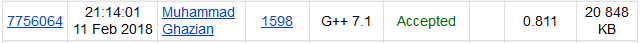
\includegraphics[scale=0.6]{bab5/img/bsgs-verdict}
	\caption{Umpan Balik Online Judge Metode \textit{Baby-Step Giant-Step}}
	\label{fig:verdict_bsgs}
\end{figure}
\end{enumerate}

Pada kode sumber dengan metode \textit{Pollard Rho}, didapat umpan balik \textit{Time Limit Exceeded}. Mengingat pengujian kebenaran untuk metode \textit{Pollard Rho} tidak dapat dilakukan menggunakan pengujian luar, pengujian lokal akan digunakan. Hasil pengujian metode tersebut untuk setiap kelompok masukan dapat dilihat pada tabel \ref{tab:test_result_fixed_l} dan \ref{tab:test_result_fixed_n}.

\begin{table}[h!]
\caption{Uji Kebenaran Metode Pollard Rho Dengan Data Masukan L Tetap}
\label{tab:test_result_fixed_l}
\begin{tabularx} {\linewidth}{ |l l X X|l l X X| }
\hline
N	&L	&Jumlah Kasus Uji	&Jumlah Benar	&N	&L	&Jumlah Kasus Uji	&Jumlah Benar \\
\hline
10	&60	&10					&10				&30	&60	&10					&10 \\
11	&60	&10					&10				&31	&60	&10					&10 \\
12	&60	&10					&10				&32	&60	&10					&10 \\
13	&60	&10					&10				&33	&60	&10					&10 \\
14	&60	&10					&10				&34	&60	&10					&10 \\
15	&60	&10					&10				&35	&60	&10					&10 \\
16	&60	&10					&10				&36	&60	&10					&10 \\
17	&60	&10					&10				&37	&60	&10					&10 \\
18	&60	&10					&10				&38	&60	&10					&10 \\
19	&60	&10					&10				&39	&60	&10					&10 \\
20	&60	&10					&10				&40	&60	&10					&10 \\
21	&60	&10					&10				&41	&60	&10					&10 \\
22	&60	&10					&10				&42	&60	&10					&10 \\
23	&60	&10					&10				&43	&60	&10					&10 \\
24	&60	&10					&10				&44	&60	&10					&10 \\
25	&60	&10					&10				&45	&60	&10					&10 \\
26	&60	&10					&10				&46	&60	&10					&10 \\
27	&60	&10					&10				&47	&60	&10					&10 \\
28	&60	&10					&10				&48	&60	&10					&10 \\
29	&60	&10					&10				&49	&60	&10					&10 \\
\hline
\end{tabularx}
\end{table}
\pagebreak

\begin{table}[h!]
\caption{Uji Kebenaran Pollard Rho Dengan Data Masukan N Tetap}
\label{tab:test_result_fixed_n}
\begin{tabularx} {\linewidth}{ |l l X X|l l X X| }
\hline
N	&L	&Jumlah Kasus Uji	&Jumlah Benar	&N	&L	&Jumlah Kasus Uji	&Jumlah Benar \\
\hline
10	&13	&7					&7				&10	&37	&10					&10 \\
10	&14	&8					&8				&10	&38	&10					&10 \\
10	&15	&10					&10				&10	&39	&10					&10 \\
10	&16	&10					&10				&10	&40	&10					&10 \\
10	&17	&10					&10				&10	&41	&10					&10 \\
10	&18	&10					&10				&10	&42	&10					&10 \\
10	&19	&10					&10				&10	&43	&10					&10 \\
10	&20	&10					&10				&10	&44	&10					&10 \\
10	&21	&10					&10				&10	&45	&10					&10 \\
10	&22	&10					&10				&10	&46	&10					&10 \\
10	&23	&10					&10				&10	&47	&10					&10 \\
10	&24	&10					&10				&10	&48	&10					&10 \\
10	&25	&10					&10				&10	&49	&10					&10 \\
10	&26	&10					&10				&10	&50	&10					&10 \\
10	&27	&10					&10				&10	&51	&10					&10 \\
10	&28	&10					&10				&10	&52	&10					&10 \\
10	&29	&10					&10				&10	&53	&10					&10 \\
10	&30	&10					&10				&10	&54	&10					&10 \\
10	&31	&10					&10				&10	&55	&10					&10 \\
10	&32	&10					&10				&10	&56	&10					&10 \\
10	&33	&10					&10				&10	&57	&10					&10 \\
10	&34	&10					&10				&10	&58	&10					&10 \\
10	&35	&10					&10				&10	&59	&10					&10 \\
10	&36	&10					&10				&10	&60	&10					&10 \\
\hline
\end{tabularx}
\end{table}
\pagebreak

Perhatikan bahwa di tabel \ref{tab:test_result_fixed_l} dan \ref{tab:test_result_fixed_n} nilai jumlah benar setiap kelompok masukan (yaitu pasangan N dan L) selalu sama dengan jumlah kasus uji yang digunakan. Maka dari itu, disimpulkan bahwa metode \textit{Pollard Rho} yang digunakan memberikan hasil yang benar. Detail terkait pengujian ini dapat dilihat pada lampiran A dan lampiran B.

\section{Uji Coba Kinerja}

Subbab ini akan menjabarkan kinerja setiap metode dengan lebih mendalam. Uji coba kinerja dilakukan melalui pengujian lokal. Menggunakan kasus uji yang sama dengan kasus uji pada subbab \ref{sec:Uji Coba Kebenaran}, akan dilakukan pengukuran waktu yang dibutuhkan untuk menyelesaikan permasalahan untuk setiap metode.

\subsection{Pengujian Menggunakan Parameter Masukan dengan N Tetap}

Pengujian menggunakan parameter masukan dengan $ N $ tetap dilakukan dengan langkah berikut.
\begin{enumerate}
	\item Rekam waktu tepat sebelum komputasi penyelesaian masalah dilakukan.
	\item Lakukan komputasi terkait penyelesaian masalah untuk sebuah masukan yang sama sebanyak 10000 kali secara berturut-turut
	\item Rekam waktu tepat setelah komputasi penyelesaian masalah dilakukan.
	\item Kurangi waktu saat selesai komputasi dengan waktu saat sebelum komputasi.
	\item Ulangi untuk seluruh kasus uji.
\end{enumerate}

Prosedur ini penting untuk dilakukan untuk memperjelas fluktuasi waktu yang dibutuhkan dalam menyelesaikan permasalahan. Keluaran prosedur ini yaitu lamanya waktu yang dibutuhkan untuk menyelesaikan permasalahan untuk 10000 kali percobaan. Perlu diperhatikan bahwa penggunaan metode \textit{Pollard Rho} menggunakan fungsi \textit{pseudorandom}, sehingga satu kali percobaan menggunakan metode \textit{Pollard Rho} sangat mungkin menghasilkan waktu yang berbeda.

\begin{figure}[h!]
	\Centering
	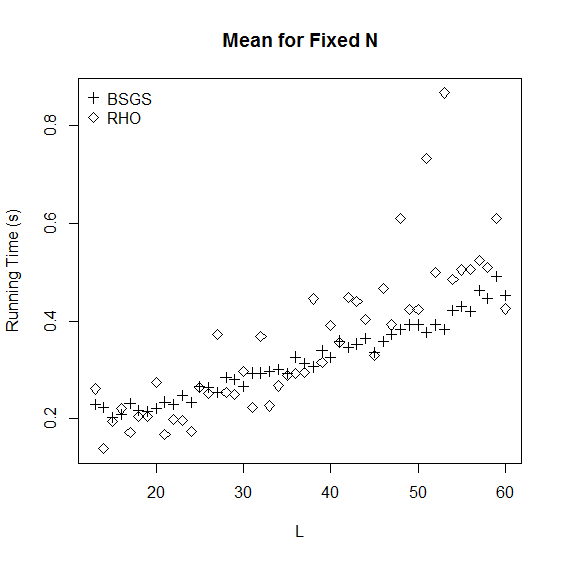
\includegraphics[angle=0, scale=0.55]{bab5/img/mean-fixed-n}
	\caption{Grafik Rata-rata Kinerja Dua Metode Untuk Kelompok Masukan N Tetap}
	\label{fig:mean_fixed_n}
\end{figure}

Grafik \ref{fig:mean_fixed_n} menampilkan rata-rata kinerja masing-masing metode apabila parameter masukan N bernilai tetap. Pada grafik tersebut dapat dilihat bahwa rata-rata \textit{running time} yang dimiliki kedua metode tidak berbeda jauh. Pada sekitar $ L \geq 40 $, rata-rata \textit{running time} metode \textit{Pollard Rho} cenderung lebih besar daripada \textit{Baby-step Giant-step}. Selain itu, \textit{running time} metode \textit{Pollard Rho} pada $ L \geq 40 $ cenderung berpencar, kontras dengan \textit{running time} \textit{Baby-step Giant-step} yang cenderung stabil.

Pertanyaan berikutnya adalah seberapa dekat \textit{running time} yang akan didapat antara rata-rata kinerja metode dengan \textit{actual running time} untuk kelompok masukan tertentu. Pertanyaan ini dapat dijawab dengan grafik 
\ref{fig:stddev_fixed_n}.

\begin{figure}[h!]
	\Centering
	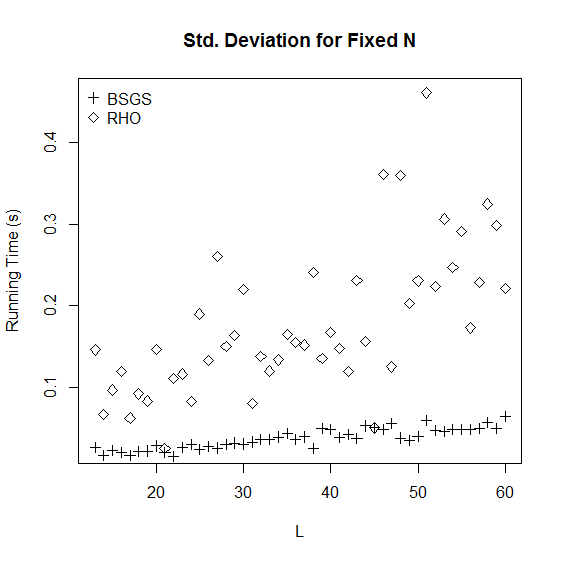
\includegraphics[angle=0, scale=0.55]{bab5/img/sdev-fixed-n}
	\caption{Grafik Standar Deviasi Kinerja Dua Metode Untuk Kelompok Masukan N Tetap}
	\label{fig:stddev_fixed_n}
\end{figure}

Pada grafik \ref{fig:stddev_fixed_n}, standar deviasi metode \textit{Pollard Rho} selalu berada di atas metode \textit{Baby-step Giant-step}. Standar deviasi metode \textit{Pollard Rho} juga relatif tinggi untuk kelompok masukan N tetap, namun masih di bawah batas atas permasalahan yaitu 1 detik. Di sisi lain, metode \textit{Baby-step Giant-step} memiliki standar deviasi yang kecil (kurang dari 0.1 detik). Artinya, metode \textit{Baby-step Giant-step} apabila digunakan untuk kelompok masukan N tetap akan menghasilkan \textit{running time} yang tidak jauh dari rata-rata \textit{running time} kelompok masukan N tersebut.

Secara umum, dampak besarnya L terhadap pertumbuhan \textit{running time} permasalahan untuk dua metode tersebut tidak begitu besar: hingga L terbesar yang mematuhi batasan soal, rata-rata \textit{running time} kedua metode tidak ada yang mencapai 1 detik. Selain itu, pertumbuhan fungsi rata-rata kedua metode cenderung linear.

\subsection{Pengujian Menggunakan Parameter Masukan dengan L Tetap}

Grafik perbandingan kinerja dua metode (\ref{fig:mean_fixed_l} dan \ref{fig:stddev_fixed_l})untuk parameter masukan dengan nilai $ L $ tetap.

\begin{figure}[h!]
	\Centering
	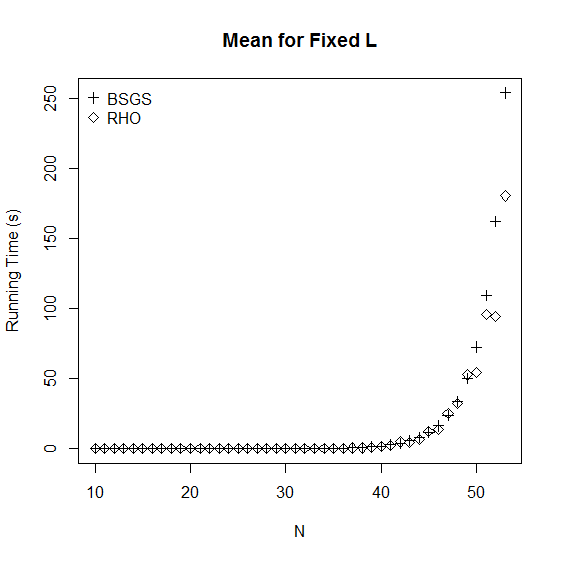
\includegraphics[angle=0, scale=0.55]{bab5/img/mean-fixed-l}
	\caption{Grafik Rata-rata Kinerja Dua Metode Untuk Kelompok Masukan L Tetap}
	\label{fig:mean_fixed_l}
\end{figure}

Grafik \ref{fig:mean_fixed_l} menunjukkan bahwa kedua metode memiliki pertumbuhan fungsi yang relatif sama. Pada $ N \geq 40 $, kedua grafik mulai melonjak naik. Namun terdapat sedikit perbedaan antar keduanya, yaitu metode rata-rata \textit{running time} \textit{Pollard Rho} lebih kecil daripada \textit{Baby-step Giant-step}. Berikutnya, grafik \ref{fig:stddev_fixed_l} akan menjelaskan mengenai standar deviasi kedua metode.

\begin{figure}[h!]
	\Centering
	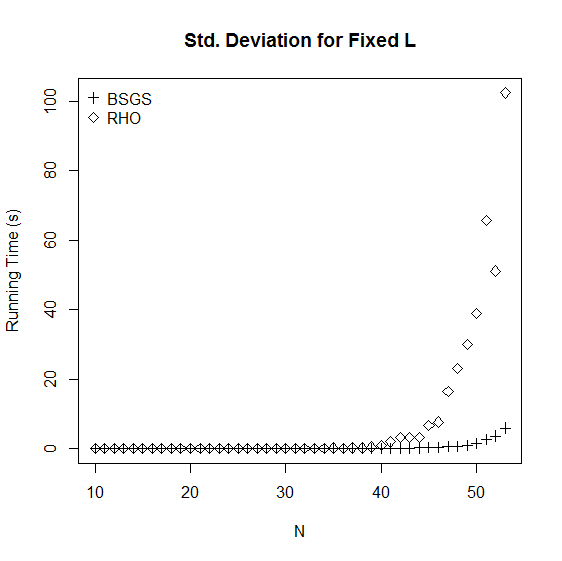
\includegraphics[angle=0, scale=0.55]{bab5/img/sdev-fixed-l}
	\caption{Grafik Standar Deviasi Kinerja Dua Metode Untuk Kelompok Masukan L Tetap}
	\label{fig:stddev_fixed_l}
\end{figure}

Berdasarkan grafik \ref{fig:stddev_fixed_l}, pertumbuhan fungsi standar deviasi kedua metode kontras dengan pertumbuhan fungsi rata-rata kedua metode. Pertumbuhan standar deviasi metode \textit{Pollard Rho} lebih besar dibanding metode \textit{Baby-step Giant-step}. Hal ini dapat dilihat pada $ N \geq 40 $.

Dari kedua pengujian kinerja terdapat kesamaan antara kedua metode terlepas dari jenis masukan yang digunakan.

\begin{enumerate}
	\item Rata-rata kinerja metode \textit{Baby-step Giant-step} dan \textit{Pollard Rho} relatif sama
	\item Standar deviasi metode \textit{Pollard Rho} cenderung lebih tinggi daripada \textit{Baby-step Giant-step}
	\item Fungsi pertumbuhan standar deviasi suatu metode sama dengan fungsi pertumbuhan rata-rata metode tersebut
\end{enumerate}

Selain itu berdasarkan uji kinerja dapat ditarik beberapa kesimpulan terkait waktu yang dibutuhkan untuk menyelesaikan permasalahan.

\begin{enumerate}
	\item Penyelesaian permasalahan dengan \textit{Baby-step Giant-step} akan membutuhkan waktu yang mendekati rata-rata \textit{running time} untuk kelompok masukan tersebut
	\item Penyelesaian permasalahan dengan \textit{Pollard Rho} dapat berjalan jauh lebih cepat atau jauh lebih lambat dari rata-rata \textit{running time} untuk kelompok masukan tersebut
	\item Besarnya L memiliki pengaruh yang tidak begitu signifikan terhadap lamanya waktu penyelesaian
	\item Besarnya N memiliki pengaruh yang signifikan terhadap lama waktu penyelesaian
\end{enumerate} \cleardoublepage
		\chapter{KESIMPULAN}

Berdasarkan penjabaran di bab-bab sebelumnya, dapat disimpulkan beberapa poin terkait penyelesaian permasalahan DSA Attack.
\begin{enumerate}
\item Permasalahan pembuatan \textit{signature} menggunakan kunci publik tanpa mengetahui kunci privat dapat diselesaikan menggunakan \textit{Baby-step Giant-step}, perkalian modular dengan \textit{Logarithmic Modular Multiplication}, pemangkatan modular dengan \textit{Repeated Squaring}, dan pencarian invers modulus dengan \textit{Extended Euclidean} dengan kompleksitas waktu sebesar $ O(\sqrt{q} \log p) + O (\log k * \log p) + O(\log k + \log p) $.
\item Metode \textit{Pollard Rho} kurang cocok digunakan sebagai solusi penyelesaian permasalahan DSA Attack karena kemungkinan waktu yang dibutuhkan bisa sangat tinggi.
\item Penyelesaian permasalahan dengan \textit{Baby-step Giant-step} akan membutuhkan waktu yang mendekati rata-rata \textit{running time} yang dimiliki metode tersebut.
\end{enumerate} \cleardoublepage
	
	\backmatter
		\printbibliography
		\chapter{LAMPIRAN A: Hasil Pengujian Untuk Kelompok N Tetap}

\newcounter{tablepart}
\setcounter{tablepart}{1}
\setcounter{table}{0}
\renewcommand{\thetable}{A.\arabic{table}}

\begin{table}[h!]
\Centering
\caption{Tabel hasil pengujian untuk kelompok N tetap (bg. \arabic{tablepart})}
\stepcounter{tablepart}
\begin{testtable}
1	&333	&99	&PASS	&333	&99	&PASS	\\
2	&178	&199	&PASS	&178	&199	&PASS	\\
3	&111	&406	&PASS	&111	&406	&PASS	\\
4	&684	&631	&PASS	&684	&631	&PASS	\\
5	&212	&33	&PASS	&212	&33	&PASS	\\
6	&256	&760	&PASS	&256	&760	&PASS	\\
7	&997	&392	&PASS	&997	&392	&PASS	\\
8	&397	&393	&PASS	&397	&393	&PASS	\\
9	&486	&323	&PASS	&486	&323	&PASS	\\
10	&477	&469	&PASS	&477	&469	&PASS	\\
11	&38	&479	&PASS	&38	&479	&PASS	\\
12	&132	&350	&PASS	&132	&350	&PASS	\\
13	&134	&781	&PASS	&134	&781	&PASS	\\
14	&638	&169	&PASS	&638	&169	&PASS	\\
15	&1013	&865	&PASS	&1013	&865	&PASS	\\
16	&517	&159	&PASS	&517	&159	&PASS	\\
17	&200	&502	&PASS	&200	&502	&PASS	\\
18	&157	&159	&PASS	&157	&159	&PASS	\\
19	&241	&272	&PASS	&241	&272	&PASS	\\
20	&111	&11	&PASS	&111	&11	&PASS	\\
21	&466	&285	&PASS	&466	&285	&PASS	\\
22	&142	&633	&PASS	&142	&633	&PASS	\\
23	&580	&394	&PASS	&580	&394	&PASS	\\
24	&344	&368	&PASS	&344	&368	&PASS	\\
25	&179	&149	&PASS	&179	&149	&PASS	\\
\end{testtable}
\end{table}
\begin{table}[h!]
\Centering
\caption{Tabel hasil pengujian untuk kelompok N tetap (bg. \arabic{tablepart})}
\stepcounter{tablepart}
\begin{testtable}
26	&476	&152	&PASS	&476	&152	&PASS	\\
27	&68	&140	&PASS	&68	&140	&PASS	\\
28	&372	&351	&PASS	&372	&351	&PASS	\\
29	&195	&371	&PASS	&195	&371	&PASS	\\
30	&535	&532	&PASS	&535	&532	&PASS	\\
31	&485	&437	&PASS	&485	&437	&PASS	\\
32	&122	&573	&PASS	&122	&573	&PASS	\\
33	&590	&508	&PASS	&590	&508	&PASS	\\
34	&58	&389	&PASS	&58	&389	&PASS	\\
35	&194	&189	&PASS	&194	&189	&PASS	\\
36	&69	&20	&PASS	&69	&20	&PASS	\\
37	&277	&423	&PASS	&277	&423	&PASS	\\
38	&463	&8	&PASS	&463	&8	&PASS	\\
39	&126	&249	&PASS	&126	&249	&PASS	\\
40	&253	&360	&PASS	&253	&360	&PASS	\\
41	&121	&249	&PASS	&121	&249	&PASS	\\
42	&203	&283	&PASS	&203	&283	&PASS	\\
43	&126	&356	&PASS	&126	&356	&PASS	\\
44	&470	&385	&PASS	&470	&385	&PASS	\\
45	&36	&568	&PASS	&36	&568	&PASS	\\
46	&433	&494	&PASS	&433	&494	&PASS	\\
47	&107	&546	&PASS	&107	&546	&PASS	\\
48	&395	&509	&PASS	&395	&509	&PASS	\\
49	&37	&224	&PASS	&37	&224	&PASS	\\
50	&125	&75	&PASS	&125	&75	&PASS	\\
\end{testtable}
\end{table}
\begin{table}[h!]
\Centering
\caption{Tabel hasil pengujian untuk kelompok N tetap (bg. \arabic{tablepart})}
\stepcounter{tablepart}
\begin{testtable}
51	&321	&118	&PASS	&321	&118	&PASS	\\
52	&128	&214	&PASS	&128	&214	&PASS	\\
53	&32	&542	&PASS	&32	&542	&PASS	\\
54	&165	&305	&PASS	&165	&305	&PASS	\\
55	&224	&228	&PASS	&224	&228	&PASS	\\
56	&132	&51	&PASS	&132	&51	&PASS	\\
57	&284	&14	&PASS	&284	&14	&PASS	\\
58	&250	&352	&PASS	&250	&352	&PASS	\\
59	&165	&363	&PASS	&165	&363	&PASS	\\
60	&488	&464	&PASS	&488	&464	&PASS	\\
61	&56	&312	&PASS	&56	&312	&PASS	\\
62	&469	&98	&PASS	&469	&98	&PASS	\\
63	&415	&359	&PASS	&415	&359	&PASS	\\
64	&546	&173	&PASS	&546	&173	&PASS	\\
65	&480	&534	&PASS	&480	&534	&PASS	\\
66	&415	&257	&PASS	&415	&257	&PASS	\\
67	&144	&267	&PASS	&144	&267	&PASS	\\
68	&500	&434	&PASS	&500	&434	&PASS	\\
69	&336	&235	&PASS	&336	&235	&PASS	\\
70	&281	&68	&PASS	&281	&68	&PASS	\\
71	&293	&88	&PASS	&293	&88	&PASS	\\
72	&500	&539	&PASS	&500	&539	&PASS	\\
73	&264	&510	&PASS	&264	&510	&PASS	\\
74	&534	&253	&PASS	&534	&253	&PASS	\\
75	&457	&501	&PASS	&457	&501	&PASS	\\
\end{testtable}
\end{table}
\begin{table}[h!]
\Centering
\caption{Tabel hasil pengujian untuk kelompok N tetap (bg. \arabic{tablepart})}
\stepcounter{tablepart}
\begin{testtable}
76	&465	&253	&PASS	&465	&253	&PASS	\\
77	&226	&365	&PASS	&226	&365	&PASS	\\
78	&467	&62	&PASS	&467	&62	&PASS	\\
79	&421	&276	&PASS	&421	&276	&PASS	\\
80	&284	&127	&PASS	&284	&127	&PASS	\\
81	&340	&419	&PASS	&340	&419	&PASS	\\
82	&256	&216	&PASS	&256	&216	&PASS	\\
83	&325	&89	&PASS	&325	&89	&PASS	\\
84	&446	&243	&PASS	&446	&243	&PASS	\\
85	&332	&427	&PASS	&332	&427	&PASS	\\
86	&355	&290	&PASS	&355	&290	&PASS	\\
87	&170	&119	&PASS	&170	&119	&PASS	\\
88	&521	&29	&PASS	&521	&29	&PASS	\\
89	&299	&484	&PASS	&299	&484	&PASS	\\
90	&37	&274	&PASS	&37	&274	&PASS	\\
91	&485	&504	&PASS	&485	&504	&PASS	\\
92	&204	&392	&PASS	&204	&392	&PASS	\\
93	&476	&466	&PASS	&476	&466	&PASS	\\
94	&291	&546	&PASS	&291	&546	&PASS	\\
95	&302	&318	&PASS	&302	&318	&PASS	\\
96	&357	&190	&PASS	&357	&190	&PASS	\\
97	&180	&385	&PASS	&180	&385	&PASS	\\
98	&102	&301	&PASS	&102	&301	&PASS	\\
99	&429	&124	&PASS	&429	&124	&PASS	\\
100	&430	&402	&PASS	&430	&402	&PASS	\\
\end{testtable}
\end{table}
\begin{table}[h!]
\Centering
\caption{Tabel hasil pengujian untuk kelompok N tetap (bg. \arabic{tablepart})}
\stepcounter{tablepart}
\begin{testtable}
101	&156	&537	&PASS	&156	&537	&PASS	\\
102	&5	&239	&PASS	&5	&239	&PASS	\\
103	&260	&379	&PASS	&260	&379	&PASS	\\
104	&38	&459	&PASS	&38	&459	&PASS	\\
105	&33	&447	&PASS	&33	&447	&PASS	\\
106	&473	&105	&PASS	&473	&105	&PASS	\\
107	&198	&327	&PASS	&198	&327	&PASS	\\
108	&264	&123	&PASS	&264	&123	&PASS	\\
109	&22	&247	&PASS	&22	&247	&PASS	\\
110	&364	&168	&PASS	&364	&168	&PASS	\\
111	&319	&494	&PASS	&319	&494	&PASS	\\
112	&131	&30	&PASS	&131	&30	&PASS	\\
113	&281	&45	&PASS	&281	&45	&PASS	\\
114	&34	&297	&PASS	&34	&297	&PASS	\\
115	&102	&15	&PASS	&102	&15	&PASS	\\
116	&86	&151	&PASS	&86	&151	&PASS	\\
117	&289	&463	&PASS	&289	&463	&PASS	\\
118	&543	&473	&PASS	&543	&473	&PASS	\\
119	&225	&531	&PASS	&225	&531	&PASS	\\
120	&240	&174	&PASS	&240	&174	&PASS	\\
121	&140	&99	&PASS	&140	&99	&PASS	\\
122	&57	&323	&PASS	&57	&323	&PASS	\\
123	&65	&46	&PASS	&65	&46	&PASS	\\
124	&528	&302	&PASS	&528	&302	&PASS	\\
125	&77	&356	&PASS	&77	&356	&PASS	\\
\end{testtable}
\end{table}
\begin{table}[h!]
\Centering
\caption{Tabel hasil pengujian untuk kelompok N tetap (bg. \arabic{tablepart})}
\stepcounter{tablepart}
\begin{testtable}
126	&158	&241	&PASS	&158	&241	&PASS	\\
127	&76	&231	&PASS	&76	&231	&PASS	\\
128	&179	&181	&PASS	&179	&181	&PASS	\\
129	&522	&114	&PASS	&522	&114	&PASS	\\
130	&247	&272	&PASS	&247	&272	&PASS	\\
131	&428	&189	&PASS	&428	&189	&PASS	\\
132	&381	&52	&PASS	&381	&52	&PASS	\\
133	&121	&144	&PASS	&121	&144	&PASS	\\
134	&267	&167	&PASS	&267	&167	&PASS	\\
135	&428	&114	&PASS	&428	&114	&PASS	\\
136	&228	&281	&PASS	&228	&281	&PASS	\\
137	&351	&126	&PASS	&351	&126	&PASS	\\
138	&151	&535	&PASS	&151	&535	&PASS	\\
139	&523	&432	&PASS	&523	&432	&PASS	\\
140	&262	&538	&PASS	&262	&538	&PASS	\\
141	&46	&501	&PASS	&46	&501	&PASS	\\
142	&448	&489	&PASS	&448	&489	&PASS	\\
143	&18	&186	&PASS	&18	&186	&PASS	\\
144	&416	&118	&PASS	&416	&118	&PASS	\\
145	&412	&198	&PASS	&412	&198	&PASS	\\
146	&382	&397	&PASS	&382	&397	&PASS	\\
147	&107	&429	&PASS	&107	&429	&PASS	\\
148	&242	&215	&PASS	&242	&215	&PASS	\\
149	&238	&126	&PASS	&238	&126	&PASS	\\
150	&299	&349	&PASS	&299	&349	&PASS	\\
\end{testtable}
\end{table}
\begin{table}[h!]
\Centering
\caption{Tabel hasil pengujian untuk kelompok N tetap (bg. \arabic{tablepart})}
\stepcounter{tablepart}
\begin{testtable}
151	&221	&345	&PASS	&221	&345	&PASS	\\
152	&306	&26	&PASS	&306	&26	&PASS	\\
153	&510	&374	&PASS	&510	&374	&PASS	\\
154	&266	&163	&PASS	&266	&163	&PASS	\\
155	&376	&229	&PASS	&376	&229	&PASS	\\
156	&423	&401	&PASS	&423	&401	&PASS	\\
157	&11	&221	&PASS	&11	&221	&PASS	\\
158	&18	&22	&PASS	&18	&22	&PASS	\\
159	&353	&334	&PASS	&353	&334	&PASS	\\
160	&69	&46	&PASS	&69	&46	&PASS	\\
161	&373	&418	&PASS	&373	&418	&PASS	\\
162	&105	&478	&PASS	&105	&478	&PASS	\\
163	&382	&21	&PASS	&382	&21	&PASS	\\
164	&119	&529	&PASS	&119	&529	&PASS	\\
165	&348	&448	&PASS	&348	&448	&PASS	\\
166	&296	&84	&PASS	&296	&84	&PASS	\\
167	&493	&72	&PASS	&493	&72	&PASS	\\
168	&74	&287	&PASS	&74	&287	&PASS	\\
169	&349	&423	&PASS	&349	&423	&PASS	\\
170	&399	&427	&PASS	&399	&427	&PASS	\\
171	&538	&187	&PASS	&538	&187	&PASS	\\
172	&110	&349	&PASS	&110	&349	&PASS	\\
173	&359	&105	&PASS	&359	&105	&PASS	\\
174	&176	&187	&PASS	&176	&187	&PASS	\\
175	&335	&208	&PASS	&335	&208	&PASS	\\
\end{testtable}
\end{table}
\begin{table}[h!]
\Centering
\caption{Tabel hasil pengujian untuk kelompok N tetap (bg. \arabic{tablepart})}
\stepcounter{tablepart}
\begin{testtable}
176	&212	&469	&PASS	&212	&469	&PASS	\\
177	&439	&516	&PASS	&439	&516	&PASS	\\
178	&237	&394	&PASS	&237	&394	&PASS	\\
179	&239	&303	&PASS	&239	&303	&PASS	\\
180	&279	&323	&PASS	&279	&323	&PASS	\\
181	&327	&135	&PASS	&327	&135	&PASS	\\
182	&282	&163	&PASS	&282	&163	&PASS	\\
183	&503	&306	&PASS	&503	&306	&PASS	\\
184	&387	&362	&PASS	&387	&362	&PASS	\\
185	&543	&284	&PASS	&543	&284	&PASS	\\
186	&247	&182	&PASS	&247	&182	&PASS	\\
187	&141	&342	&PASS	&141	&342	&PASS	\\
188	&231	&38	&PASS	&231	&38	&PASS	\\
189	&244	&91	&PASS	&244	&91	&PASS	\\
190	&80	&422	&PASS	&80	&422	&PASS	\\
191	&189	&71	&PASS	&189	&71	&PASS	\\
192	&426	&427	&PASS	&426	&427	&PASS	\\
193	&357	&172	&PASS	&357	&172	&PASS	\\
194	&526	&43	&PASS	&526	&43	&PASS	\\
195	&492	&483	&PASS	&492	&483	&PASS	\\
196	&137	&23	&PASS	&137	&23	&PASS	\\
197	&528	&91	&PASS	&528	&91	&PASS	\\
198	&216	&492	&PASS	&216	&492	&PASS	\\
199	&360	&147	&PASS	&360	&147	&PASS	\\
200	&309	&96	&PASS	&309	&96	&PASS	\\
\end{testtable}
\end{table}
\begin{table}[h!]
\Centering
\caption{Tabel hasil pengujian untuk kelompok N tetap (bg. \arabic{tablepart})}
\stepcounter{tablepart}
\begin{testtable}
201	&526	&311	&PASS	&526	&311	&PASS	\\
202	&431	&287	&PASS	&431	&287	&PASS	\\
203	&307	&323	&PASS	&307	&323	&PASS	\\
204	&390	&90	&PASS	&390	&90	&PASS	\\
205	&333	&186	&PASS	&333	&186	&PASS	\\
206	&207	&365	&PASS	&207	&365	&PASS	\\
207	&71	&437	&PASS	&71	&437	&PASS	\\
208	&243	&246	&PASS	&243	&246	&PASS	\\
209	&6	&189	&PASS	&6	&189	&PASS	\\
210	&470	&314	&PASS	&470	&314	&PASS	\\
211	&53	&417	&PASS	&53	&417	&PASS	\\
212	&162	&535	&PASS	&162	&535	&PASS	\\
213	&529	&266	&PASS	&529	&266	&PASS	\\
214	&426	&484	&PASS	&426	&484	&PASS	\\
215	&490	&69	&PASS	&490	&69	&PASS	\\
216	&502	&251	&PASS	&502	&251	&PASS	\\
217	&129	&16	&PASS	&129	&16	&PASS	\\
218	&121	&519	&PASS	&121	&519	&PASS	\\
219	&154	&173	&PASS	&154	&173	&PASS	\\
220	&74	&452	&PASS	&74	&452	&PASS	\\
221	&395	&464	&PASS	&395	&464	&PASS	\\
222	&450	&56	&PASS	&450	&56	&PASS	\\
223	&52	&207	&PASS	&52	&207	&PASS	\\
224	&168	&153	&PASS	&168	&153	&PASS	\\
225	&363	&244	&PASS	&363	&244	&PASS	\\
\end{testtable}
\end{table}
\begin{table}[h!]
\Centering
\caption{Tabel hasil pengujian untuk kelompok N tetap (bg. \arabic{tablepart})}
\stepcounter{tablepart}
\begin{testtable}
226	&441	&454	&PASS	&441	&454	&PASS	\\
227	&163	&376	&PASS	&163	&376	&PASS	\\
228	&237	&109	&PASS	&237	&109	&PASS	\\
229	&493	&84	&PASS	&493	&84	&PASS	\\
230	&118	&149	&PASS	&118	&149	&PASS	\\
231	&252	&8	&PASS	&252	&8	&PASS	\\
232	&346	&340	&PASS	&346	&340	&PASS	\\
233	&304	&389	&PASS	&304	&389	&PASS	\\
234	&320	&266	&PASS	&320	&266	&PASS	\\
235	&334	&432	&PASS	&334	&432	&PASS	\\
236	&404	&135	&PASS	&404	&135	&PASS	\\
237	&29	&217	&PASS	&29	&217	&PASS	\\
238	&346	&64	&PASS	&346	&64	&PASS	\\
239	&523	&431	&PASS	&523	&431	&PASS	\\
240	&192	&140	&PASS	&192	&140	&PASS	\\
241	&90	&256	&PASS	&90	&256	&PASS	\\
242	&139	&442	&PASS	&139	&442	&PASS	\\
243	&219	&443	&PASS	&219	&443	&PASS	\\
244	&522	&148	&PASS	&522	&148	&PASS	\\
245	&341	&524	&PASS	&341	&524	&PASS	\\
246	&296	&249	&PASS	&296	&249	&PASS	\\
247	&472	&271	&PASS	&472	&271	&PASS	\\
248	&417	&419	&PASS	&417	&419	&PASS	\\
249	&179	&473	&PASS	&179	&473	&PASS	\\
250	&178	&129	&PASS	&178	&129	&PASS	\\
\end{testtable}
\end{table}
\begin{table}[h!]
\Centering
\caption{Tabel hasil pengujian untuk kelompok N tetap (bg. \arabic{tablepart})}
\stepcounter{tablepart}
\begin{testtable}
251	&327	&129	&PASS	&327	&129	&PASS	\\
252	&243	&361	&PASS	&243	&361	&PASS	\\
253	&543	&204	&PASS	&543	&204	&PASS	\\
254	&207	&215	&PASS	&207	&215	&PASS	\\
255	&61	&24	&PASS	&61	&24	&PASS	\\
256	&503	&20	&PASS	&503	&20	&PASS	\\
257	&356	&543	&PASS	&356	&543	&PASS	\\
258	&461	&195	&PASS	&461	&195	&PASS	\\
259	&542	&497	&PASS	&542	&497	&PASS	\\
260	&531	&148	&PASS	&531	&148	&PASS	\\
261	&515	&244	&PASS	&515	&244	&PASS	\\
262	&191	&380	&PASS	&191	&380	&PASS	\\
263	&124	&117	&PASS	&124	&117	&PASS	\\
264	&431	&238	&PASS	&431	&238	&PASS	\\
265	&508	&54	&PASS	&508	&54	&PASS	\\
266	&114	&335	&PASS	&114	&335	&PASS	\\
267	&210	&387	&PASS	&210	&387	&PASS	\\
268	&30	&487	&PASS	&30	&487	&PASS	\\
269	&13	&61	&PASS	&13	&61	&PASS	\\
270	&323	&177	&PASS	&323	&177	&PASS	\\
271	&229	&527	&PASS	&229	&527	&PASS	\\
272	&67	&188	&PASS	&67	&188	&PASS	\\
273	&511	&178	&PASS	&511	&178	&PASS	\\
274	&360	&292	&PASS	&360	&292	&PASS	\\
275	&424	&186	&PASS	&424	&186	&PASS	\\
\end{testtable}
\end{table}
\begin{table}[h!]
\Centering
\caption{Tabel hasil pengujian untuk kelompok N tetap (bg. \arabic{tablepart})}
\stepcounter{tablepart}
\begin{testtable}
276	&198	&291	&PASS	&198	&291	&PASS	\\
277	&332	&121	&PASS	&332	&121	&PASS	\\
278	&249	&76	&PASS	&249	&76	&PASS	\\
279	&525	&61	&PASS	&525	&61	&PASS	\\
280	&230	&447	&PASS	&230	&447	&PASS	\\
281	&119	&498	&PASS	&119	&498	&PASS	\\
282	&479	&251	&PASS	&479	&251	&PASS	\\
283	&532	&220	&PASS	&532	&220	&PASS	\\
284	&349	&164	&PASS	&349	&164	&PASS	\\
285	&492	&173	&PASS	&492	&173	&PASS	\\
286	&207	&79	&PASS	&207	&79	&PASS	\\
287	&514	&315	&PASS	&514	&315	&PASS	\\
288	&351	&540	&PASS	&351	&540	&PASS	\\
289	&344	&249	&PASS	&344	&249	&PASS	\\
290	&309	&264	&PASS	&309	&264	&PASS	\\
291	&246	&427	&PASS	&246	&427	&PASS	\\
292	&280	&30	&PASS	&280	&30	&PASS	\\
293	&75	&477	&PASS	&75	&477	&PASS	\\
294	&436	&372	&PASS	&436	&372	&PASS	\\
295	&300	&304	&PASS	&300	&304	&PASS	\\
296	&501	&102	&PASS	&501	&102	&PASS	\\
297	&273	&275	&PASS	&273	&275	&PASS	\\
298	&269	&103	&PASS	&269	&103	&PASS	\\
299	&514	&65	&PASS	&514	&65	&PASS	\\
300	&419	&195	&PASS	&419	&195	&PASS	\\
\end{testtable}
\end{table}
\begin{table}[h!]
\Centering
\caption{Tabel hasil pengujian untuk kelompok N tetap (bg. \arabic{tablepart})}
\stepcounter{tablepart}
\begin{testtable}
301	&541	&478	&PASS	&541	&478	&PASS	\\
302	&112	&237	&PASS	&112	&237	&PASS	\\
303	&38	&59	&PASS	&38	&59	&PASS	\\
304	&518	&101	&PASS	&518	&101	&PASS	\\
305	&48	&421	&PASS	&48	&421	&PASS	\\
306	&97	&339	&PASS	&97	&339	&PASS	\\
307	&117	&275	&PASS	&117	&275	&PASS	\\
308	&535	&220	&PASS	&535	&220	&PASS	\\
309	&266	&136	&PASS	&266	&136	&PASS	\\
310	&159	&391	&PASS	&159	&391	&PASS	\\
311	&391	&144	&PASS	&391	&144	&PASS	\\
312	&55	&458	&PASS	&55	&458	&PASS	\\
313	&209	&218	&PASS	&209	&218	&PASS	\\
314	&482	&50	&PASS	&482	&50	&PASS	\\
315	&544	&237	&PASS	&544	&237	&PASS	\\
316	&39	&92	&PASS	&39	&92	&PASS	\\
317	&346	&472	&PASS	&346	&472	&PASS	\\
318	&268	&178	&PASS	&268	&178	&PASS	\\
319	&251	&293	&PASS	&251	&293	&PASS	\\
320	&424	&311	&PASS	&424	&311	&PASS	\\
321	&304	&468	&PASS	&304	&468	&PASS	\\
322	&62	&539	&PASS	&62	&539	&PASS	\\
323	&231	&546	&PASS	&231	&546	&PASS	\\
324	&93	&227	&PASS	&93	&227	&PASS	\\
325	&176	&193	&PASS	&176	&193	&PASS	\\
\end{testtable}
\end{table}
\begin{table}[h!]
\Centering
\caption{Tabel hasil pengujian untuk kelompok N tetap (bg. \arabic{tablepart})}
\stepcounter{tablepart}
\begin{testtable}
326	&137	&291	&PASS	&137	&291	&PASS	\\
327	&479	&51	&PASS	&479	&51	&PASS	\\
328	&446	&86	&PASS	&446	&86	&PASS	\\
329	&315	&100	&PASS	&315	&100	&PASS	\\
330	&100	&536	&PASS	&100	&536	&PASS	\\
331	&88	&150	&PASS	&88	&150	&PASS	\\
332	&438	&346	&PASS	&438	&346	&PASS	\\
333	&505	&13	&PASS	&505	&13	&PASS	\\
334	&190	&189	&PASS	&190	&189	&PASS	\\
335	&278	&43	&PASS	&278	&43	&PASS	\\
336	&175	&76	&PASS	&175	&76	&PASS	\\
337	&381	&537	&PASS	&381	&537	&PASS	\\
338	&292	&216	&PASS	&292	&216	&PASS	\\
339	&401	&428	&PASS	&401	&428	&PASS	\\
340	&407	&1	&PASS	&407	&1	&PASS	\\
341	&433	&493	&PASS	&433	&493	&PASS	\\
342	&476	&56	&PASS	&476	&56	&PASS	\\
343	&481	&406	&PASS	&481	&406	&PASS	\\
344	&44	&36	&PASS	&44	&36	&PASS	\\
345	&430	&224	&PASS	&430	&224	&PASS	\\
346	&17	&483	&PASS	&17	&483	&PASS	\\
347	&304	&469	&PASS	&304	&469	&PASS	\\
348	&437	&3	&PASS	&437	&3	&PASS	\\
349	&256	&170	&PASS	&256	&170	&PASS	\\
350	&283	&145	&PASS	&283	&145	&PASS	\\
\end{testtable}
\end{table}
\begin{table}[h!]
\Centering
\caption{Tabel hasil pengujian untuk kelompok N tetap (bg. \arabic{tablepart})}
\stepcounter{tablepart}
\begin{testtable}
351	&499	&143	&PASS	&499	&143	&PASS	\\
352	&90	&71	&PASS	&90	&71	&PASS	\\
353	&46	&118	&PASS	&46	&118	&PASS	\\
354	&23	&143	&PASS	&23	&143	&PASS	\\
355	&268	&531	&PASS	&268	&531	&PASS	\\
356	&534	&310	&PASS	&534	&310	&PASS	\\
357	&443	&244	&PASS	&443	&244	&PASS	\\
358	&20	&55	&PASS	&20	&55	&PASS	\\
359	&477	&333	&PASS	&477	&333	&PASS	\\
360	&151	&355	&PASS	&151	&355	&PASS	\\
361	&256	&59	&PASS	&256	&59	&PASS	\\
362	&241	&235	&PASS	&241	&235	&PASS	\\
363	&268	&70	&PASS	&268	&70	&PASS	\\
364	&536	&50	&PASS	&536	&50	&PASS	\\
365	&430	&208	&PASS	&430	&208	&PASS	\\
366	&332	&303	&PASS	&332	&303	&PASS	\\
367	&204	&42	&PASS	&204	&42	&PASS	\\
368	&537	&278	&PASS	&537	&278	&PASS	\\
369	&233	&399	&PASS	&233	&399	&PASS	\\
370	&178	&377	&PASS	&178	&377	&PASS	\\
371	&196	&297	&PASS	&196	&297	&PASS	\\
372	&148	&237	&PASS	&148	&237	&PASS	\\
373	&421	&450	&PASS	&421	&450	&PASS	\\
374	&472	&449	&PASS	&472	&449	&PASS	\\
375	&286	&140	&PASS	&286	&140	&PASS	\\
\end{testtable}
\end{table}
\begin{table}[h!]
\Centering
\caption{Tabel hasil pengujian untuk kelompok N tetap (bg. \arabic{tablepart})}
\stepcounter{tablepart}
\begin{testtable}
376	&237	&138	&PASS	&237	&138	&PASS	\\
377	&133	&397	&PASS	&133	&397	&PASS	\\
378	&37	&405	&PASS	&37	&405	&PASS	\\
379	&209	&176	&PASS	&209	&176	&PASS	\\
380	&348	&123	&PASS	&348	&123	&PASS	\\
381	&309	&374	&PASS	&309	&374	&PASS	\\
382	&314	&444	&PASS	&314	&444	&PASS	\\
383	&492	&226	&PASS	&492	&226	&PASS	\\
384	&505	&297	&PASS	&505	&297	&PASS	\\
385	&149	&153	&PASS	&149	&153	&PASS	\\
386	&211	&480	&PASS	&211	&480	&PASS	\\
387	&446	&481	&PASS	&446	&481	&PASS	\\
388	&133	&292	&PASS	&133	&292	&PASS	\\
389	&349	&67	&PASS	&349	&67	&PASS	\\
390	&234	&345	&PASS	&234	&345	&PASS	\\
391	&183	&376	&PASS	&183	&376	&PASS	\\
392	&527	&496	&PASS	&527	&496	&PASS	\\
393	&244	&213	&PASS	&244	&213	&PASS	\\
394	&435	&395	&PASS	&435	&395	&PASS	\\
395	&197	&218	&PASS	&197	&218	&PASS	\\
396	&398	&412	&PASS	&398	&412	&PASS	\\
397	&97	&85	&PASS	&97	&85	&PASS	\\
398	&470	&494	&PASS	&470	&494	&PASS	\\
399	&77	&23	&PASS	&77	&23	&PASS	\\
400	&338	&468	&PASS	&338	&468	&PASS	\\
\end{testtable}
\end{table}
\begin{table}[h!]
\Centering
\caption{Tabel hasil pengujian untuk kelompok N tetap (bg. \arabic{tablepart})}
\stepcounter{tablepart}
\begin{testtable}
401	&478	&34	&PASS	&478	&34	&PASS	\\
402	&412	&86	&PASS	&412	&86	&PASS	\\
403	&163	&202	&PASS	&163	&202	&PASS	\\
404	&469	&9	&PASS	&469	&9	&PASS	\\
405	&301	&126	&PASS	&301	&126	&PASS	\\
406	&33	&408	&PASS	&33	&408	&PASS	\\
407	&70	&35	&PASS	&70	&35	&PASS	\\
408	&176	&363	&PASS	&176	&363	&PASS	\\
409	&312	&496	&PASS	&312	&496	&PASS	\\
410	&249	&215	&PASS	&249	&215	&PASS	\\
411	&173	&172	&PASS	&173	&172	&PASS	\\
412	&204	&5	&PASS	&204	&5	&PASS	\\
413	&165	&358	&PASS	&165	&358	&PASS	\\
414	&180	&192	&PASS	&180	&192	&PASS	\\
415	&495	&481	&PASS	&495	&481	&PASS	\\
416	&38	&357	&PASS	&38	&357	&PASS	\\
417	&250	&525	&PASS	&250	&525	&PASS	\\
418	&237	&358	&PASS	&237	&358	&PASS	\\
419	&257	&286	&PASS	&257	&286	&PASS	\\
420	&98	&196	&PASS	&98	&196	&PASS	\\
421	&244	&267	&PASS	&244	&267	&PASS	\\
422	&458	&482	&PASS	&458	&482	&PASS	\\
423	&348	&6	&PASS	&348	&6	&PASS	\\
424	&334	&182	&PASS	&334	&182	&PASS	\\
425	&265	&262	&PASS	&265	&262	&PASS	\\
\end{testtable}
\end{table}
\begin{table}[h!]
\Centering
\caption{Tabel hasil pengujian untuk kelompok N tetap (bg. \arabic{tablepart})}
\stepcounter{tablepart}
\begin{testtable}
426	&313	&197	&PASS	&313	&197	&PASS	\\
427	&516	&243	&PASS	&516	&243	&PASS	\\
428	&54	&137	&PASS	&54	&137	&PASS	\\
429	&253	&76	&PASS	&253	&76	&PASS	\\
430	&492	&531	&PASS	&492	&531	&PASS	\\
431	&235	&379	&PASS	&235	&379	&PASS	\\
432	&1	&113	&PASS	&1	&113	&PASS	\\
433	&353	&31	&PASS	&353	&31	&PASS	\\
434	&73	&537	&PASS	&73	&537	&PASS	\\
435	&242	&135	&PASS	&242	&135	&PASS	\\
436	&131	&332	&PASS	&131	&332	&PASS	\\
437	&190	&340	&PASS	&190	&340	&PASS	\\
438	&155	&238	&PASS	&155	&238	&PASS	\\
439	&243	&277	&PASS	&243	&277	&PASS	\\
440	&11	&224	&PASS	&11	&224	&PASS	\\
441	&143	&100	&PASS	&143	&100	&PASS	\\
442	&414	&541	&PASS	&414	&541	&PASS	\\
443	&421	&177	&PASS	&421	&177	&PASS	\\
444	&376	&534	&PASS	&376	&534	&PASS	\\
445	&35	&393	&PASS	&35	&393	&PASS	\\
446	&148	&331	&PASS	&148	&331	&PASS	\\
447	&273	&48	&PASS	&273	&48	&PASS	\\
448	&194	&433	&PASS	&194	&433	&PASS	\\
449	&155	&465	&PASS	&155	&465	&PASS	\\
450	&82	&311	&PASS	&82	&311	&PASS	\\
\end{testtable}
\end{table}
\begin{table}[h!]
\Centering
\caption{Tabel hasil pengujian untuk kelompok N tetap (bg. \arabic{tablepart})}
\stepcounter{tablepart}
\begin{testtable}
451	&186	&505	&PASS	&186	&505	&PASS	\\
452	&35	&394	&PASS	&35	&394	&PASS	\\
453	&75	&3	&PASS	&75	&3	&PASS	\\
454	&308	&150	&PASS	&308	&150	&PASS	\\
455	&382	&413	&PASS	&382	&413	&PASS	\\
456	&372	&287	&PASS	&372	&287	&PASS	\\
457	&419	&110	&PASS	&419	&110	&PASS	\\
458	&469	&48	&PASS	&469	&48	&PASS	\\
459	&538	&49	&PASS	&538	&49	&PASS	\\
460	&224	&107	&PASS	&224	&107	&PASS	\\
461	&104	&277	&PASS	&104	&277	&PASS	\\
462	&513	&198	&PASS	&513	&198	&PASS	\\
463	&378	&294	&PASS	&378	&294	&PASS	\\
464	&257	&156	&PASS	&257	&156	&PASS	\\
465	&222	&363	&PASS	&222	&363	&PASS	\\
466	&109	&471	&PASS	&109	&471	&PASS	\\
467	&51	&511	&PASS	&51	&511	&PASS	\\
468	&478	&228	&PASS	&478	&228	&PASS	\\
469	&248	&469	&PASS	&248	&469	&PASS	\\
470	&6	&314	&PASS	&6	&314	&PASS	\\
471	&198	&369	&PASS	&198	&369	&PASS	\\
472	&240	&108	&PASS	&240	&108	&PASS	\\
473	&228	&68	&PASS	&228	&68	&PASS	\\
474	&149	&394	&PASS	&149	&394	&PASS	\\
475	&25	&378	&PASS	&25	&378	&PASS	\\
\end{testtable}
\end{table}
		\chapter{LAMPIRAN B: Hasil Pengujian Untuk Kelompok L Tetap}

\setcounter{tablepart}{1}
\setcounter{table}{0}
\renewcommand{\thetable}{B.\arabic{table}}

\begin{table}[h!]
\Centering
\caption{Tabel hasil pengujian untuk kelompok N tetap (bg. \arabic{tablepart})}
\stepcounter{tablepart}
\begin{testtable}
1	&109	&541	&PASS	&109	&541	&PASS	\\
2	&51	&285	&PASS	&51	&285	&PASS	\\
3	&478	&376	&PASS	&478	&376	&PASS	\\
4	&248	&195	&PASS	&248	&195	&PASS	\\
5	&6	&24	&PASS	&6	&24	&PASS	\\
6	&198	&129	&PASS	&198	&129	&PASS	\\
7	&240	&494	&PASS	&240	&494	&PASS	\\
8	&228	&39	&PASS	&228	&39	&PASS	\\
9	&149	&202	&PASS	&149	&202	&PASS	\\
10	&25	&465	&PASS	&25	&465	&PASS	\\
11	&1002	&338	&PASS	&1002	&338	&PASS	\\
12	&830	&980	&PASS	&830	&980	&PASS	\\
13	&699	&693	&PASS	&699	&693	&PASS	\\
14	&573	&853	&PASS	&573	&853	&PASS	\\
15	&202	&461	&PASS	&202	&461	&PASS	\\
16	&960	&72	&PASS	&960	&72	&PASS	\\
17	&237	&724	&PASS	&237	&724	&PASS	\\
18	&528	&718	&PASS	&528	&718	&PASS	\\
19	&675	&78	&PASS	&675	&78	&PASS	\\
20	&170	&692	&PASS	&170	&692	&PASS	\\
21	&1353	&1607	&PASS	&1353	&1607	&PASS	\\
22	&950	&1134	&PASS	&950	&1134	&PASS	\\
23	&1269	&1820	&PASS	&1269	&1820	&PASS	\\
24	&858	&753	&PASS	&858	&753	&PASS	\\
25	&1512	&2014	&PASS	&1512	&2014	&PASS	\\
\end{testtable}
\end{table}
\begin{table}[h!]
\Centering
\caption{Tabel hasil pengujian untuk kelompok N tetap (bg. \arabic{tablepart})}
\stepcounter{tablepart}
\begin{testtable}
26	&1327	&698	&PASS	&1327	&698	&PASS	\\
27	&663	&1144	&PASS	&663	&1144	&PASS	\\
28	&1706	&77	&PASS	&1706	&77	&PASS	\\
29	&1332	&2083	&PASS	&1332	&2083	&PASS	\\
30	&1012	&1057	&PASS	&1012	&1057	&PASS	\\
31	&498	&2767	&PASS	&498	&2767	&PASS	\\
32	&1068	&3418	&PASS	&1068	&3418	&PASS	\\
33	&3613	&238	&PASS	&3613	&238	&PASS	\\
34	&759	&3252	&PASS	&759	&3252	&PASS	\\
35	&1115	&1580	&PASS	&1115	&1580	&PASS	\\
36	&379	&137	&PASS	&379	&137	&PASS	\\
37	&528	&576	&PASS	&528	&576	&PASS	\\
38	&3506	&2935	&PASS	&3506	&2935	&PASS	\\
39	&3508	&3113	&PASS	&3508	&3113	&PASS	\\
40	&3653	&735	&PASS	&3653	&735	&PASS	\\
41	&5898	&2012	&PASS	&5898	&2012	&PASS	\\
42	&5251	&7545	&PASS	&5251	&7545	&PASS	\\
43	&4692	&4724	&PASS	&4692	&4724	&PASS	\\
44	&4712	&3848	&PASS	&4712	&3848	&PASS	\\
45	&2630	&1695	&PASS	&2630	&1695	&PASS	\\
46	&2285	&8031	&PASS	&2285	&8031	&PASS	\\
47	&3800	&5225	&PASS	&3800	&5225	&PASS	\\
48	&1213	&515	&PASS	&1213	&515	&PASS	\\
49	&4767	&4156	&PASS	&4767	&4156	&PASS	\\
50	&1256	&106	&PASS	&1256	&106	&PASS	\\
\end{testtable}
\end{table}
\begin{table}[h!]
\Centering
\caption{Tabel hasil pengujian untuk kelompok N tetap (bg. \arabic{tablepart})}
\stepcounter{tablepart}
\begin{testtable}
51	&3938	&2324	&PASS	&3938	&2324	&PASS	\\
52	&10688	&13518	&PASS	&10688	&13518	&PASS	\\
53	&2518	&3102	&PASS	&2518	&3102	&PASS	\\
54	&7213	&4570	&PASS	&7213	&4570	&PASS	\\
55	&11443	&4971	&PASS	&11443	&4971	&PASS	\\
56	&14736	&8664	&PASS	&14736	&8664	&PASS	\\
57	&616	&9672	&PASS	&616	&9672	&PASS	\\
58	&13610	&15765	&PASS	&13610	&15765	&PASS	\\
59	&9148	&2658	&PASS	&9148	&2658	&PASS	\\
60	&10354	&10865	&PASS	&10354	&10865	&PASS	\\
61	&32865	&21567	&PASS	&32865	&21567	&PASS	\\
62	&17371	&17041	&PASS	&17371	&17041	&PASS	\\
63	&17091	&13632	&PASS	&17091	&13632	&PASS	\\
64	&24894	&21677	&PASS	&24894	&21677	&PASS	\\
65	&24134	&26932	&PASS	&24134	&26932	&PASS	\\
66	&7464	&24248	&PASS	&7464	&24248	&PASS	\\
67	&24418	&25151	&PASS	&24418	&25151	&PASS	\\
68	&8520	&18746	&PASS	&8520	&18746	&PASS	\\
69	&18946	&494	&PASS	&18946	&494	&PASS	\\
70	&20082	&14747	&PASS	&20082	&14747	&PASS	\\
71	&40041	&38151	&PASS	&40041	&38151	&PASS	\\
72	&28665	&53134	&PASS	&28665	&53134	&PASS	\\
73	&56242	&21508	&PASS	&56242	&21508	&PASS	\\
74	&55689	&53756	&PASS	&55689	&53756	&PASS	\\
75	&42511	&30448	&PASS	&42511	&30448	&PASS	\\
\end{testtable}
\end{table}
\begin{table}[h!]
\Centering
\caption{Tabel hasil pengujian untuk kelompok N tetap (bg. \arabic{tablepart})}
\stepcounter{tablepart}
\begin{testtable}
76	&56416	&22516	&PASS	&56416	&22516	&PASS	\\
77	&20370	&65537	&PASS	&20370	&65537	&PASS	\\
78	&37776	&12030	&PASS	&37776	&12030	&PASS	\\
79	&5151	&58176	&PASS	&5151	&58176	&PASS	\\
80	&27415	&53192	&PASS	&27415	&53192	&PASS	\\
81	&117815	&49879	&PASS	&117815	&49879	&PASS	\\
82	&38977	&110802	&PASS	&38977	&110802	&PASS	\\
83	&95404	&13712	&PASS	&95404	&13712	&PASS	\\
84	&114494	&83109	&PASS	&114494	&83109	&PASS	\\
85	&98695	&81235	&PASS	&98695	&81235	&PASS	\\
86	&121234	&59371	&PASS	&121234	&59371	&PASS	\\
87	&25906	&35431	&PASS	&25906	&35431	&PASS	\\
88	&103773	&98744	&PASS	&103773	&98744	&PASS	\\
89	&98369	&18734	&PASS	&98369	&18734	&PASS	\\
90	&62918	&53945	&PASS	&62918	&53945	&PASS	\\
91	&81121	&26175	&PASS	&81121	&26175	&PASS	\\
92	&81955	&140985	&PASS	&81955	&140985	&PASS	\\
93	&255369	&115304	&PASS	&255369	&115304	&PASS	\\
94	&78800	&228116	&PASS	&78800	&228116	&PASS	\\
95	&114674	&72778	&PASS	&114674	&72778	&PASS	\\
96	&88285	&221843	&PASS	&88285	&221843	&PASS	\\
97	&176452	&119326	&PASS	&176452	&119326	&PASS	\\
98	&84677	&223315	&PASS	&84677	&223315	&PASS	\\
99	&93932	&145509	&PASS	&93932	&145509	&PASS	\\
100	&80916	&113876	&PASS	&80916	&113876	&PASS	\\
\end{testtable}
\end{table}
\begin{table}[h!]
\Centering
\caption{Tabel hasil pengujian untuk kelompok N tetap (bg. \arabic{tablepart})}
\stepcounter{tablepart}
\begin{testtable}
101	&47615	&208662	&PASS	&47615	&208662	&PASS	\\
102	&361854	&311289	&PASS	&361854	&311289	&PASS	\\
103	&285727	&25936	&PASS	&285727	&25936	&PASS	\\
104	&368670	&422121	&PASS	&368670	&422121	&PASS	\\
105	&196251	&305328	&PASS	&196251	&305328	&PASS	\\
106	&9185	&506580	&PASS	&9185	&506580	&PASS	\\
107	&245546	&475206	&PASS	&245546	&475206	&PASS	\\
108	&197716	&440801	&PASS	&197716	&440801	&PASS	\\
109	&200244	&65539	&PASS	&200244	&65539	&PASS	\\
110	&58109	&517360	&PASS	&58109	&517360	&PASS	\\
111	&22883	&39374	&PASS	&22883	&39374	&PASS	\\
112	&855435	&292024	&PASS	&855435	&292024	&PASS	\\
113	&607155	&1010677	&PASS	&607155	&1010677	&PASS	\\
114	&365780	&631057	&PASS	&365780	&631057	&PASS	\\
115	&522342	&622348	&PASS	&522342	&622348	&PASS	\\
116	&1575	&12061	&PASS	&1575	&12061	&PASS	\\
117	&765335	&378131	&PASS	&765335	&378131	&PASS	\\
118	&700212	&769390	&PASS	&700212	&769390	&PASS	\\
119	&771756	&395187	&PASS	&771756	&395187	&PASS	\\
120	&520374	&272742	&PASS	&520374	&272742	&PASS	\\
121	&2084454	&1519736	&PASS	&2084454	&1519736	&PASS	\\
122	&1572832	&1513382	&PASS	&1572832	&1513382	&PASS	\\
123	&628681	&708786	&PASS	&628681	&708786	&PASS	\\
124	&1261487	&1325647	&PASS	&1261487	&1325647	&PASS	\\
125	&1882434	&1389074	&PASS	&1882434	&1389074	&PASS	\\
\end{testtable}
\end{table}
\begin{table}[h!]
\Centering
\caption{Tabel hasil pengujian untuk kelompok N tetap (bg. \arabic{tablepart})}
\stepcounter{tablepart}
\begin{testtable}
126	&288467	&424841	&PASS	&288467	&424841	&PASS	\\
127	&374224	&1331802	&PASS	&374224	&1331802	&PASS	\\
128	&23660	&240233	&PASS	&23660	&240233	&PASS	\\
129	&1315830	&283350	&PASS	&1315830	&283350	&PASS	\\
130	&1101837	&1977372	&PASS	&1101837	&1977372	&PASS	\\
131	&1680879	&3842373	&PASS	&1680879	&3842373	&PASS	\\
132	&3952542	&4102497	&PASS	&3952542	&4102497	&PASS	\\
133	&3566820	&1922644	&PASS	&3566820	&1922644	&PASS	\\
134	&76137	&3331004	&PASS	&76137	&3331004	&PASS	\\
135	&445444	&4015249	&PASS	&445444	&4015249	&PASS	\\
136	&3056421	&3596924	&PASS	&3056421	&3596924	&PASS	\\
137	&3845065	&3080891	&PASS	&3845065	&3080891	&PASS	\\
138	&2287024	&369263	&PASS	&2287024	&369263	&PASS	\\
139	&164181	&2436398	&PASS	&164181	&2436398	&PASS	\\
140	&1747747	&3874737	&PASS	&1747747	&3874737	&PASS	\\
141	&1305828	&5581042	&PASS	&1305828	&5581042	&PASS	\\
142	&6095465	&47667	&PASS	&6095465	&47667	&PASS	\\
143	&5579802	&4107238	&PASS	&5579802	&4107238	&PASS	\\
144	&6167423	&7468993	&PASS	&6167423	&7468993	&PASS	\\
145	&319633	&7681693	&PASS	&319633	&7681693	&PASS	\\
146	&2384286	&4002367	&PASS	&2384286	&4002367	&PASS	\\
147	&7626619	&5531871	&PASS	&7626619	&5531871	&PASS	\\
148	&5365686	&542642	&PASS	&5365686	&542642	&PASS	\\
149	&6837360	&506293	&PASS	&6837360	&506293	&PASS	\\
150	&2212133	&6143708	&PASS	&2212133	&6143708	&PASS	\\
\end{testtable}
\end{table}
\begin{landscape}
\begin{table}[h!]
\Centering
\caption{Tabel hasil pengujian untuk kelompok N tetap (bg. \arabic{tablepart})}
\stepcounter{tablepart}
\begin{testtable}
151	&10138100	&6589945	&PASS	&10138100	&6589945	&PASS	\\
152	&5662161	&2672069	&PASS	&5662161	&2672069	&PASS	\\
153	&1358619	&12918553	&PASS	&1358619	&12918553	&PASS	\\
154	&16154373	&16627699	&PASS	&16154373	&16627699	&PASS	\\
155	&11057074	&7882574	&PASS	&11057074	&7882574	&PASS	\\
156	&13058900	&4286437	&PASS	&13058900	&4286437	&PASS	\\
157	&12007200	&16646369	&PASS	&12007200	&16646369	&PASS	\\
158	&6319242	&6755746	&PASS	&6319242	&6755746	&PASS	\\
159	&16584342	&2236947	&PASS	&16584342	&2236947	&PASS	\\
160	&7658982	&3516685	&PASS	&7658982	&3516685	&PASS	\\
161	&9949064	&28056083	&PASS	&9949064	&28056083	&PASS	\\
162	&624198	&17144584	&PASS	&624198	&17144584	&PASS	\\
163	&12534308	&20045882	&PASS	&12534308	&20045882	&PASS	\\
164	&30728906	&26178451	&PASS	&30728906	&26178451	&PASS	\\
165	&10755464	&32804031	&PASS	&10755464	&32804031	&PASS	\\
166	&15527158	&23838698	&PASS	&15527158	&23838698	&PASS	\\
167	&15830992	&29539660	&PASS	&15830992	&29539660	&PASS	\\
168	&30417017	&1850583	&PASS	&30417017	&1850583	&PASS	\\
\end{testtable}
\end{table}
\end{landscape}
\begin{landscape}
\begin{table}[h!]
\Centering
\caption{Tabel hasil pengujian untuk kelompok N tetap (bg. \arabic{tablepart})}
\stepcounter{tablepart}
\begin{testtable}
169	&32860134	&16632951	&PASS	&32860134	&16632951	&PASS	\\
170	&4502675	&11571054	&PASS	&4502675	&11571054	&PASS	\\
171	&16794022	&20827452	&PASS	&16794022	&20827452	&PASS	\\
172	&42632957	&10121900	&PASS	&42632957	&10121900	&PASS	\\
173	&12666970	&52140105	&PASS	&12666970	&52140105	&PASS	\\
174	&32208124	&16312879	&PASS	&32208124	&16312879	&PASS	\\
175	&18156095	&32943136	&PASS	&18156095	&32943136	&PASS	\\
176	&45182729	&26130305	&PASS	&45182729	&26130305	&PASS	\\
177	&52803250	&44551932	&PASS	&52803250	&44551932	&PASS	\\
178	&28299812	&16218241	&PASS	&28299812	&16218241	&PASS	\\
179	&29779414	&40907752	&PASS	&29779414	&40907752	&PASS	\\
180	&55881025	&22406446	&PASS	&55881025	&22406446	&PASS	\\
181	&98668838	&55031983	&PASS	&98668838	&55031983	&PASS	\\
182	&78087687	&74542798	&PASS	&78087687	&74542798	&PASS	\\
183	&10362033	&113972215	&PASS	&10362033	&113972215	&PASS	\\
184	&129180136	&83333411	&PASS	&129180136	&83333411	&PASS	\\
185	&60661690	&93331570	&PASS	&60661690	&93331570	&PASS	\\
186	&125754579	&15402793	&PASS	&125754579	&15402793	&PASS	\\
\end{testtable}
\end{table}
\end{landscape}
\begin{landscape}
\begin{table}[h!]
\Centering
\caption{Tabel hasil pengujian untuk kelompok N tetap (bg. \arabic{tablepart})}
\stepcounter{tablepart}
\begin{testtable}
187	&7071321	&93654106	&PASS	&7071321	&93654106	&PASS	\\
188	&55079978	&91764593	&PASS	&55079978	&91764593	&PASS	\\
189	&24747269	&93477858	&PASS	&24747269	&93477858	&PASS	\\
190	&2260531	&14858674	&PASS	&2260531	&14858674	&PASS	\\
191	&149213151	&165508008	&PASS	&149213151	&165508008	&PASS	\\
192	&56668243	&18210419	&PASS	&56668243	&18210419	&PASS	\\
193	&224423343	&150027430	&PASS	&224423343	&150027430	&PASS	\\
194	&38802104	&137977292	&PASS	&38802104	&137977292	&PASS	\\
195	&199495941	&29630156	&PASS	&199495941	&29630156	&PASS	\\
196	&19727024	&255138363	&PASS	&19727024	&255138363	&PASS	\\
197	&38343360	&12652194	&PASS	&38343360	&12652194	&PASS	\\
198	&246762256	&126101379	&PASS	&246762256	&126101379	&PASS	\\
199	&260563559	&15312774	&PASS	&260563559	&15312774	&PASS	\\
200	&249473251	&227764167	&PASS	&249473251	&227764167	&PASS	\\
201	&66111473	&247804757	&PASS	&66111473	&247804757	&PASS	\\
202	&338600630	&95026991	&PASS	&338600630	&95026991	&PASS	\\
203	&36196630	&509369069	&PASS	&36196630	&509369069	&PASS	\\
204	&97740482	&315139307	&PASS	&97740482	&315139307	&PASS	\\
\end{testtable}
\end{table}
\end{landscape}
\begin{landscape}
\begin{table}[h!]
\Centering
\caption{Tabel hasil pengujian untuk kelompok N tetap (bg. \arabic{tablepart})}
\stepcounter{tablepart}
\begin{testtable}
205	&500891483	&384142993	&PASS	&500891483	&384142993	&PASS	\\
206	&373948078	&267050867	&PASS	&373948078	&267050867	&PASS	\\
207	&476456552	&8183518	&PASS	&476456552	&8183518	&PASS	\\
208	&232248747	&28272436	&PASS	&232248747	&28272436	&PASS	\\
209	&139836806	&156735947	&PASS	&139836806	&156735947	&PASS	\\
210	&493685823	&289807993	&PASS	&493685823	&289807993	&PASS	\\
211	&20610716	&7699932	&PASS	&20610716	&7699932	&PASS	\\
212	&157746122	&405146495	&PASS	&157746122	&405146495	&PASS	\\
213	&986976984	&299512796	&PASS	&986976984	&299512796	&PASS	\\
214	&730292857	&469016820	&PASS	&730292857	&469016820	&PASS	\\
215	&561361343	&420496215	&PASS	&561361343	&420496215	&PASS	\\
216	&339364343	&212621209	&PASS	&339364343	&212621209	&PASS	\\
217	&667623083	&631934829	&PASS	&667623083	&631934829	&PASS	\\
218	&1027674034	&317989988	&PASS	&1027674034	&317989988	&PASS	\\
219	&268423493	&1032060677	&PASS	&268423493	&1032060677	&PASS	\\
220	&661255322	&1010624355	&PASS	&661255322	&1010624355	&PASS	\\
221	&727730147	&1908752259	&PASS	&727730147	&1908752259	&PASS	\\
222	&2070745858	&888256705	&PASS	&2070745858	&888256705	&PASS	\\
\end{testtable}
\end{table}
\end{landscape}
\begin{landscape}
\begin{table}[h!]
\Centering
\caption{Tabel hasil pengujian untuk kelompok N tetap (bg. \arabic{tablepart})}
\stepcounter{tablepart}
\begin{testtable}
223	&2014769345	&769003634	&PASS	&2014769345	&769003634	&PASS	\\
224	&541976515	&883568243	&PASS	&541976515	&883568243	&PASS	\\
225	&928190361	&728912549	&PASS	&928190361	&728912549	&PASS	\\
226	&1714048224	&1812863211	&PASS	&1714048224	&1812863211	&PASS	\\
227	&1389658460	&1220170887	&PASS	&1389658460	&1220170887	&PASS	\\
228	&402558126	&1275978503	&PASS	&402558126	&1275978503	&PASS	\\
229	&1928037864	&451449648	&PASS	&1928037864	&451449648	&PASS	\\
230	&1221108416	&1452162173	&PASS	&1221108416	&1452162173	&PASS	\\
231	&757397928	&3018697591	&PASS	&757397928	&3018697591	&PASS	\\
232	&2744476079	&1992119715	&PASS	&2744476079	&1992119715	&PASS	\\
233	&2817986240	&1955312229	&PASS	&2817986240	&1955312229	&PASS	\\
234	&3774097562	&284722153	&PASS	&3774097562	&284722153	&PASS	\\
235	&378854104	&3546440984	&PASS	&378854104	&3546440984	&PASS	\\
236	&338809105	&1188039066	&PASS	&338809105	&1188039066	&PASS	\\
237	&432786141	&2482058165	&PASS	&432786141	&2482058165	&PASS	\\
238	&2173615966	&126926672	&PASS	&2173615966	&126926672	&PASS	\\
239	&936199509	&863390944	&PASS	&936199509	&863390944	&PASS	\\
240	&3892508351	&4161265323	&PASS	&3892508351	&4161265323	&PASS	\\
\end{testtable}
\end{table}
\end{landscape}
\begin{landscape}
\begin{table}[h!]
\Centering
\caption{Tabel hasil pengujian untuk kelompok N tetap (bg. \arabic{tablepart})}
\stepcounter{tablepart}
\begin{testtable}
241	&5411606075	&7487387890	&PASS	&5411606075	&7487387890	&PASS	\\
242	&8557091865	&6355963527	&PASS	&8557091865	&6355963527	&PASS	\\
243	&6470696696	&5817026392	&PASS	&6470696696	&5817026392	&PASS	\\
244	&6817234544	&990699110	&PASS	&6817234544	&990699110	&PASS	\\
245	&4846560477	&3780767617	&PASS	&4846560477	&3780767617	&PASS	\\
246	&2389655437	&602797344	&PASS	&2389655437	&602797344	&PASS	\\
247	&5129303288	&8068198307	&PASS	&5129303288	&8068198307	&PASS	\\
248	&8117876828	&4865562041	&PASS	&8117876828	&4865562041	&PASS	\\
249	&7913114616	&3211813974	&PASS	&7913114616	&3211813974	&PASS	\\
250	&3646532133	&118686715	&PASS	&3646532133	&118686715	&PASS	\\
251	&6401965709	&12335276051	&PASS	&6401965709	&12335276051	&PASS	\\
252	&9662053471	&4187734040	&PASS	&9662053471	&4187734040	&PASS	\\
253	&4099905326	&14040740883	&PASS	&4099905326	&14040740883	&PASS	\\
254	&10772658924	&3180789427	&PASS	&10772658924	&3180789427	&PASS	\\
255	&16057687460	&16732553972	&PASS	&16057687460	&16732553972	&PASS	\\
256	&10258918645	&2887809885	&PASS	&10258918645	&2887809885	&PASS	\\
257	&12922017974	&9855266773	&PASS	&12922017974	&9855266773	&PASS	\\
258	&16047631521	&14924220331	&PASS	&16047631521	&14924220331	&PASS	\\
\end{testtable}
\end{table}
\end{landscape}
\begin{landscape}
\begin{table}[h!]
\Centering
\caption{Tabel hasil pengujian untuk kelompok N tetap (bg. \arabic{tablepart})}
\stepcounter{tablepart}
\begin{testtable}
259	&6673198260	&10407484594	&PASS	&6673198260	&10407484594	&PASS	\\
260	&12987464746	&10684795969	&PASS	&12987464746	&10684795969	&PASS	\\
261	&32392213496	&2284276442	&PASS	&32392213496	&2284276442	&PASS	\\
262	&19744592908	&31420919598	&PASS	&19744592908	&31420919598	&PASS	\\
263	&9433797427	&26687433143	&PASS	&9433797427	&26687433143	&PASS	\\
264	&9987401922	&25633750966	&PASS	&9987401922	&25633750966	&PASS	\\
265	&13207218049	&1226330109	&PASS	&13207218049	&1226330109	&PASS	\\
266	&7260112393	&9553348648	&PASS	&7260112393	&9553348648	&PASS	\\
267	&26468377776	&25441822034	&PASS	&26468377776	&25441822034	&PASS	\\
268	&23430727682	&11012722057	&PASS	&23430727682	&11012722057	&PASS	\\
269	&21757301159	&28703817164	&PASS	&21757301159	&28703817164	&PASS	\\
270	&26955065162	&8357197191	&PASS	&26955065162	&8357197191	&PASS	\\
271	&65356889029	&41726158387	&PASS	&65356889029	&41726158387	&PASS	\\
272	&18574408430	&32855411145	&PASS	&18574408430	&32855411145	&PASS	\\
273	&41826311486	&67907459992	&PASS	&41826311486	&67907459992	&PASS	\\
274	&56276237745	&55902395677	&PASS	&56276237745	&55902395677	&PASS	\\
275	&419156830	&40587986800	&PASS	&419156830	&40587986800	&PASS	\\
276	&63461291315	&18858235083	&PASS	&63461291315	&18858235083	&PASS	\\
\end{testtable}
\end{table}
\end{landscape}
\begin{landscape}
\begin{table}[h!]
\Centering
\caption{Tabel hasil pengujian untuk kelompok N tetap (bg. \arabic{tablepart})}
\stepcounter{tablepart}
\begin{testtable}
277	&35873514486	&51482284981	&PASS	&35873514486	&51482284981	&PASS	\\
278	&54158512529	&24319060283	&PASS	&54158512529	&24319060283	&PASS	\\
279	&10786300467	&46083337553	&PASS	&10786300467	&46083337553	&PASS	\\
280	&41684118191	&22782602677	&PASS	&41684118191	&22782602677	&PASS	\\
281	&95023432987	&25468740874	&PASS	&95023432987	&25468740874	&PASS	\\
282	&9700349094	&73143227774	&PASS	&9700349094	&73143227774	&PASS	\\
283	&29259223743	&72776048315	&PASS	&29259223743	&72776048315	&PASS	\\
284	&88050811440	&8767846263	&PASS	&88050811440	&8767846263	&PASS	\\
285	&12625122444	&92926985367	&PASS	&12625122444	&92926985367	&PASS	\\
286	&107288244985	&20035505627	&PASS	&107288244985	&20035505627	&PASS	\\
287	&26878262769	&62682103674	&PASS	&26878262769	&62682103674	&PASS	\\
288	&123128706419	&83757171839	&PASS	&123128706419	&83757171839	&PASS	\\
289	&99907283853	&68890558965	&PASS	&99907283853	&68890558965	&PASS	\\
290	&49413183432	&35008674708	&PASS	&49413183432	&35008674708	&PASS	\\
291	&116303586398	&194653178784	&PASS	&116303586398	&194653178784	&PASS	\\
292	&81403150984	&37255091036	&PASS	&81403150984	&37255091036	&PASS	\\
293	&182413485979	&100917836432	&PASS	&182413485979	&100917836432	&PASS	\\
294	&251862127077	&191069743767	&PASS	&251862127077	&191069743767	&PASS	\\
\end{testtable}
\end{table}
\end{landscape}
\begin{landscape}
\begin{table}[h!]
\Centering
\caption{Tabel hasil pengujian untuk kelompok N tetap (bg. \arabic{tablepart})}
\stepcounter{tablepart}
\begin{testtable}
295	&47648955330	&165713328822	&PASS	&47648955330	&165713328822	&PASS	\\
296	&138683002321	&212828698111	&PASS	&138683002321	&212828698111	&PASS	\\
297	&74045161501	&24334440671	&PASS	&74045161501	&24334440671	&PASS	\\
298	&44859094925	&240441507040	&PASS	&44859094925	&240441507040	&PASS	\\
299	&226799322382	&145369102659	&PASS	&226799322382	&145369102659	&PASS	\\
300	&154485710098	&251596713885	&PASS	&154485710098	&251596713885	&PASS	\\
301	&353088968850	&61997017800	&PASS	&353088968850	&61997017800	&PASS	\\
302	&353650907119	&207521653913	&PASS	&353650907119	&207521653913	&PASS	\\
303	&354677441966	&437218278677	&PASS	&354677441966	&437218278677	&PASS	\\
304	&28808111527	&381035709519	&PASS	&28808111527	&381035709519	&PASS	\\
305	&418040386872	&307545001209	&PASS	&418040386872	&307545001209	&PASS	\\
306	&279594709982	&104628623995	&PASS	&279594709982	&104628623995	&PASS	\\
307	&527483346732	&46140811464	&PASS	&527483346732	&46140811464	&PASS	\\
308	&290433541735	&342844828995	&PASS	&290433541735	&342844828995	&PASS	\\
309	&197093187331	&508671456525	&PASS	&197093187331	&508671456525	&PASS	\\
310	&146542066515	&259721356437	&PASS	&146542066515	&259721356437	&PASS	\\
311	&426295662982	&423738933351	&PASS	&426295662982	&423738933351	&PASS	\\
312	&463247708936	&380073111677	&PASS	&463247708936	&380073111677	&PASS	\\
\end{testtable}
\end{table}
\end{landscape}
\begin{landscape}
\begin{table}[h!]
\Centering
\caption{Tabel hasil pengujian untuk kelompok N tetap (bg. \arabic{tablepart})}
\stepcounter{tablepart}
\begin{testtable}
313	&303786246628	&352097146249	&PASS	&303786246628	&352097146249	&PASS	\\
314	&490938871391	&248096594802	&PASS	&490938871391	&248096594802	&PASS	\\
315	&300580191740	&559704074165	&PASS	&300580191740	&559704074165	&PASS	\\
316	&252452296196	&116088025741	&PASS	&252452296196	&116088025741	&PASS	\\
317	&1072788830693	&70543298459	&PASS	&1072788830693	&70543298459	&PASS	\\
318	&52652485126	&835327965849	&PASS	&52652485126	&835327965849	&PASS	\\
319	&874933822573	&867992797522	&PASS	&874933822573	&867992797522	&PASS	\\
320	&547757430891	&644188034375	&PASS	&547757430891	&644188034375	&PASS	\\
321	&971451321567	&1343623479175	&PASS	&971451321567	&1343623479175	&PASS	\\
322	&1321550941271	&1241013750802	&PASS	&1321550941271	&1241013750802	&PASS	\\
323	&657205120872	&2122743806063	&PASS	&657205120872	&2122743806063	&PASS	\\
324	&1544567451385	&781548097913	&PASS	&1544567451385	&781548097913	&PASS	\\
325	&258629089825	&850521236234	&PASS	&258629089825	&850521236234	&PASS	\\
326	&913517890367	&1689054923459	&PASS	&913517890367	&1689054923459	&PASS	\\
327	&618616006473	&920404975642	&PASS	&618616006473	&920404975642	&PASS	\\
328	&2046172584371	&137507650173	&PASS	&2046172584371	&137507650173	&PASS	\\
329	&1194183833655	&552614213373	&PASS	&1194183833655	&552614213373	&PASS	\\
330	&146643046538	&320723889461	&PASS	&146643046538	&320723889461	&PASS	\\
\end{testtable}
\end{table}
\end{landscape}
\begin{landscape}
\begin{table}[h!]
\Centering
\caption{Tabel hasil pengujian untuk kelompok N tetap (bg. \arabic{tablepart})}
\stepcounter{tablepart}
\begin{testtable}
331	&2965666768226	&1944390103649	&PASS	&2965666768226	&1944390103649	&PASS	\\
332	&1518680582767	&2715339908490	&PASS	&1518680582767	&2715339908490	&PASS	\\
333	&1662163524342	&3011224237259	&PASS	&1662163524342	&3011224237259	&PASS	\\
334	&2269109326583	&4308510472347	&PASS	&2269109326583	&4308510472347	&PASS	\\
335	&3199792334103	&2147478498164	&PASS	&3199792334103	&2147478498164	&PASS	\\
336	&2427813652846	&2760612783290	&PASS	&2427813652846	&2760612783290	&PASS	\\
337	&3285802264102	&643069883064	&PASS	&3285802264102	&643069883064	&PASS	\\
338	&1141502010622	&2744455943966	&PASS	&1141502010622	&2744455943966	&PASS	\\
339	&3775083397354	&2983786538285	&PASS	&3775083397354	&2983786538285	&PASS	\\
340	&3304751448562	&1829486083367	&PASS	&3304751448562	&1829486083367	&PASS	\\
341	&8371119016287	&8307120414373	&PASS	&8371119016287	&8307120414373	&PASS	\\
342	&7544701205554	&4485789561530	&PASS	&7544701205554	&4485789561530	&PASS	\\
343	&2558294431826	&638236462599	&PASS	&2558294431826	&638236462599	&PASS	\\
344	&5248938536801	&3220718323807	&PASS	&5248938536801	&3220718323807	&PASS	\\
345	&6885504164993	&4274527756349	&PASS	&6885504164993	&4274527756349	&PASS	\\
346	&3399378043324	&1466406378015	&PASS	&3399378043324	&1466406378015	&PASS	\\
347	&7317699085753	&5482719678088	&PASS	&7317699085753	&5482719678088	&PASS	\\
348	&363354238516	&5269806511025	&PASS	&363354238516	&5269806511025	&PASS	\\
\end{testtable}
\end{table}
\end{landscape}
\begin{landscape}
\begin{table}[h!]
\small
\Centering
\caption{Tabel hasil pengujian untuk kelompok N tetap (bg. \arabic{tablepart})}
\stepcounter{tablepart}
\begin{testtable}
349	&3866812738896	&8683125135189	&PASS	&3866812738896	&8683125135189	&PASS	\\
350	&3771467340986	&8041283557193	&PASS	&3771467340986	&8041283557193	&PASS	\\
351	&9188683807847	&6965518538881	&PASS	&9188683807847	&6965518538881	&PASS	\\
352	&2367884771497	&6546446938534	&PASS	&2367884771497	&6546446938534	&PASS	\\
353	&16107401516279	&4132053454536	&PASS	&16107401516279	&4132053454536	&PASS	\\
354	&16304805141136	&15618621715633	&PASS	&16304805141136	&15618621715633	&PASS	\\
355	&1780396574738	&5117368603714	&PASS	&1780396574738	&5117368603714	&PASS	\\
356	&8676868872441	&17463690278320	&PASS	&8676868872441	&17463690278320	&PASS	\\
357	&8578981486719	&15489285466994	&PASS	&8578981486719	&15489285466994	&PASS	\\
358	&14967193637580	&4141463566791	&PASS	&14967193637580	&4141463566791	&PASS	\\
359	&4539622655438	&17133032203088	&PASS	&4539622655438	&17133032203088	&PASS	\\
360	&14080362035270	&4938487348444	&PASS	&14080362035270	&4938487348444	&PASS	\\
361	&26065509390271	&15982905740220	&PASS	&26065509390271	&15982905740220	&PASS	\\
362	&24408983558442	&26271094454805	&PASS	&24408983558442	&26271094454805	&PASS	\\
363	&3010981852188	&17437011060618	&PASS	&3010981852188	&17437011060618	&PASS	\\
364	&3716136619421	&13499700120892	&PASS	&3716136619421	&13499700120892	&PASS	\\
365	&10609409066982	&30853325887958	&PASS	&10609409066982	&30853325887958	&PASS	\\
366	&32255054294300	&13925913023585	&PASS	&32255054294300	&13925913023585	&PASS	\\
\end{testtable}
\end{table}
\end{landscape}
\begin{landscape}
\begin{table}[h!]
\small
\Centering
\caption{Tabel hasil pengujian untuk kelompok N tetap (bg. \arabic{tablepart})}
\stepcounter{tablepart}
\begin{testtable}
367	&19629535350427	&26912990294037	&PASS	&19629535350427	&26912990294037	&PASS	\\
368	&27737265824131	&2796930611731	&PASS	&27737265824131	&2796930611731	&PASS	\\
369	&16828432489273	&3016596073943	&PASS	&16828432489273	&3016596073943	&PASS	\\
370	&31585303675147	&20575060865817	&PASS	&31585303675147	&20575060865817	&PASS	\\
371	&59221930865420	&37032947987091	&PASS	&59221930865420	&37032947987091	&PASS	\\
372	&27908278410750	&26933120858130	&PASS	&27908278410750	&26933120858130	&PASS	\\
373	&1831949751110	&23618786609149	&PASS	&1831949751110	&23618786609149	&PASS	\\
374	&13876480264682	&25292398209634	&PASS	&13876480264682	&25292398209634	&PASS	\\
375	&69952861011070	&42321357771229	&PASS	&69952861011070	&42321357771229	&PASS	\\
376	&21648325987454	&69025998705367	&PASS	&21648325987454	&69025998705367	&PASS	\\
377	&16954747528682	&27237842940837	&PASS	&16954747528682	&27237842940837	&PASS	\\
378	&65602839753932	&46299196986790	&PASS	&65602839753932	&46299196986790	&PASS	\\
379	&20171238094414	&7473627332577	&PASS	&20171238094414	&7473627332577	&PASS	\\
380	&3029520761157	&64478696578872	&PASS	&3029520761157	&64478696578872	&PASS	\\
381	&136529648548473	&138073796353178	&PASS	&136529648548473	&138073796353178	&PASS	\\
382	&60991194294665	&135427868647953	&PASS	&60991194294665	&135427868647953	&PASS	\\
383	&91280776822603	&2867409488742	&PASS	&91280776822603	&2867409488742	&PASS	\\
384	&33700294856190	&124441603604579	&PASS	&33700294856190	&124441603604579	&PASS	\\
\end{testtable}
\end{table}
\end{landscape}
\begin{landscape}
\begin{table}[h!]
\small
\Centering
\caption{Tabel hasil pengujian untuk kelompok N tetap (bg. \arabic{tablepart})}
\stepcounter{tablepart}
\begin{testtable}
385	&123091770542011	&56324451709783	&PASS	&123091770542011	&56324451709783	&PASS	\\
386	&72007844093672	&44345501630291	&PASS	&72007844093672	&44345501630291	&PASS	\\
387	&38917320343255	&68174009995390	&PASS	&38917320343255	&68174009995390	&PASS	\\
388	&52607976585873	&41557780952133	&PASS	&52607976585873	&41557780952133	&PASS	\\
389	&65901799654834	&83168809807430	&PASS	&65901799654834	&83168809807430	&PASS	\\
390	&49527864301365	&80189625890905	&PASS	&49527864301365	&80189625890905	&PASS	\\
391	&272516187489891	&89885302676830	&PASS	&272516187489891	&89885302676830	&PASS	\\
392	&73473706879304	&212602400059393	&PASS	&73473706879304	&212602400059393	&PASS	\\
393	&144808394000157	&15615812063212	&PASS	&144808394000157	&15615812063212	&PASS	\\
394	&195935380344652	&54209818326353	&PASS	&195935380344652	&54209818326353	&PASS	\\
395	&17899780268273	&277177132550354	&PASS	&17899780268273	&277177132550354	&PASS	\\
396	&143309380522129	&266514401759177	&PASS	&143309380522129	&266514401759177	&PASS	\\
397	&86410287860773	&57923757436501	&PASS	&86410287860773	&57923757436501	&PASS	\\
398	&18133114508503	&280920535575155	&PASS	&18133114508503	&280920535575155	&PASS	\\
399	&92657416460148	&81586844006545	&PASS	&92657416460148	&81586844006545	&PASS	\\
400	&150558692230362	&47943495147437	&PASS	&150558692230362	&47943495147437	&PASS	\\
401	&286508033312352	&43664768558129	&PASS	&286508033312352	&43664768558129	&PASS	\\
402	&206638708008930	&268906017163358	&PASS	&206638708008930	&268906017163358	&PASS	\\
\end{testtable}
\end{table}
\end{landscape}
\begin{landscape}
\begin{table}[h!]
\small
\Centering
\caption{Tabel hasil pengujian untuk kelompok N tetap (bg. \arabic{tablepart})}
\stepcounter{tablepart}
\begin{testtable}
403	&165374958901146	&284679466996617	&PASS	&165374958901146	&284679466996617	&PASS	\\
404	&57309530696663	&453668668226624	&PASS	&57309530696663	&453668668226624	&PASS	\\
405	&127230098829927	&52376634188990	&PASS	&127230098829927	&52376634188990	&PASS	\\
406	&404292564084724	&240580835352308	&PASS	&404292564084724	&240580835352308	&PASS	\\
407	&220110332960199	&348446923572307	&PASS	&220110332960199	&348446923572307	&PASS	\\
408	&397905157794727	&110037652866013	&PASS	&397905157794727	&110037652866013	&PASS	\\
409	&510049187246945	&152005841196311	&PASS	&510049187246945	&152005841196311	&PASS	\\
410	&488193265217347	&21272666517230	&PASS	&488193265217347	&21272666517230	&PASS	\\
411	&746606505427713	&369913265956421	&PASS	&746606505427713	&369913265956421	&PASS	\\
412	&450957579547550	&244092443297566	&PASS	&450957579547550	&244092443297566	&PASS	\\
413	&38471255955117	&1078266188167050	&PASS	&38471255955117	&1078266188167050	&PASS	\\
414	&857966567236659	&698254422665847	&PASS	&857966567236659	&698254422665847	&PASS	\\
415	&212992634323097	&660645577949974	&PASS	&212992634323097	&660645577949974	&PASS	\\
416	&92283886819367	&428191139133707	&PASS	&92283886819367	&428191139133707	&PASS	\\
417	&370477018269742	&1082785449153000	&PASS	&370477018269742	&1082785449153000	&PASS	\\
418	&912444881587832	&349848960574379	&PASS	&912444881587832	&349848960574379	&PASS	\\
419	&1080351393421970	&878626919711333	&PASS	&1080351393421970	&878626919711333	&PASS	\\
420	&1012252601998050	&217912686921748	&PASS	&1012252601998050	&217912686921748	&PASS	\\
\end{testtable}
\end{table}
\end{landscape}
\begin{landscape}
\begin{table}[h!]
\small
\Centering
\caption{Tabel hasil pengujian untuk kelompok N tetap (bg. \arabic{tablepart})}
\stepcounter{tablepart}
\begin{testtable}
421	&901490465203660	&2002164777588450	&PASS	&901490465203660	&2002164777588450	&PASS	\\
422	&1699900514924990	&664866451905517	&PASS	&1699900514924990	&664866451905517	&PASS	\\
423	&375718888312327	&687125515587588	&PASS	&375718888312327	&687125515587588	&PASS	\\
424	&1200332611505010	&1746319869703150	&PASS	&1200332611505010	&1746319869703150	&PASS	\\
425	&1856063536700100	&2237991695997640	&PASS	&1856063536700100	&2237991695997640	&PASS	\\
426	&2076129577713830	&462657643170032	&PASS	&2076129577713830	&462657643170032	&PASS	\\
427	&1166628140873040	&585792920858825	&PASS	&1166628140873040	&585792920858825	&PASS	\\
428	&963390434399194	&1999977230811850	&PASS	&963390434399194	&1999977230811850	&PASS	\\
429	&1747691904904970	&1052319422873620	&PASS	&1747691904904970	&1052319422873620	&PASS	\\
430	&1934307474257550	&2186087584250900	&PASS	&1934307474257550	&2186087584250900	&PASS	\\
431	&1703250383514940	&3019586044379760	&PASS	&1703250383514940	&3019586044379760	&PASS	\\
432	&4030785952692380	&4413974923492350	&PASS	&4030785952692380	&4413974923492350	&PASS	\\
433	&3314744762791840	&202232248597497	&PASS	&3314744762791840	&202232248597497	&PASS	\\
434	&122608321780494	&187827649272142	&PASS	&122608321780494	&187827649272142	&PASS	\\
435	&313359623397328	&2337435997356020	&PASS	&313359623397328	&2337435997356020	&PASS	\\
436	&613233657957334	&3261978850243830	&PASS	&613233657957334	&3261978850243830	&PASS	\\
437	&1166938159181410	&1233145574847920	&PASS	&1166938159181410	&1233145574847920	&PASS	\\
438	&1098467589938900	&1876837674848550	&PASS	&1098467589938900	&1876837674848550	&PASS	\\
439	&257880306509642	&2678014826884840	&PASS	&257880306509642	&2678014826884840	&PASS	\\
440	&1756201523811940	&2837275479809360	&PASS	&1756201523811940	&2837275479809360	&PASS	\\
\end{testtable}
\end{table}
\end{landscape}
		\chapter{BIODATA PENULIS}

\begin{wrapfigure}{l}{0.3\textwidth}
	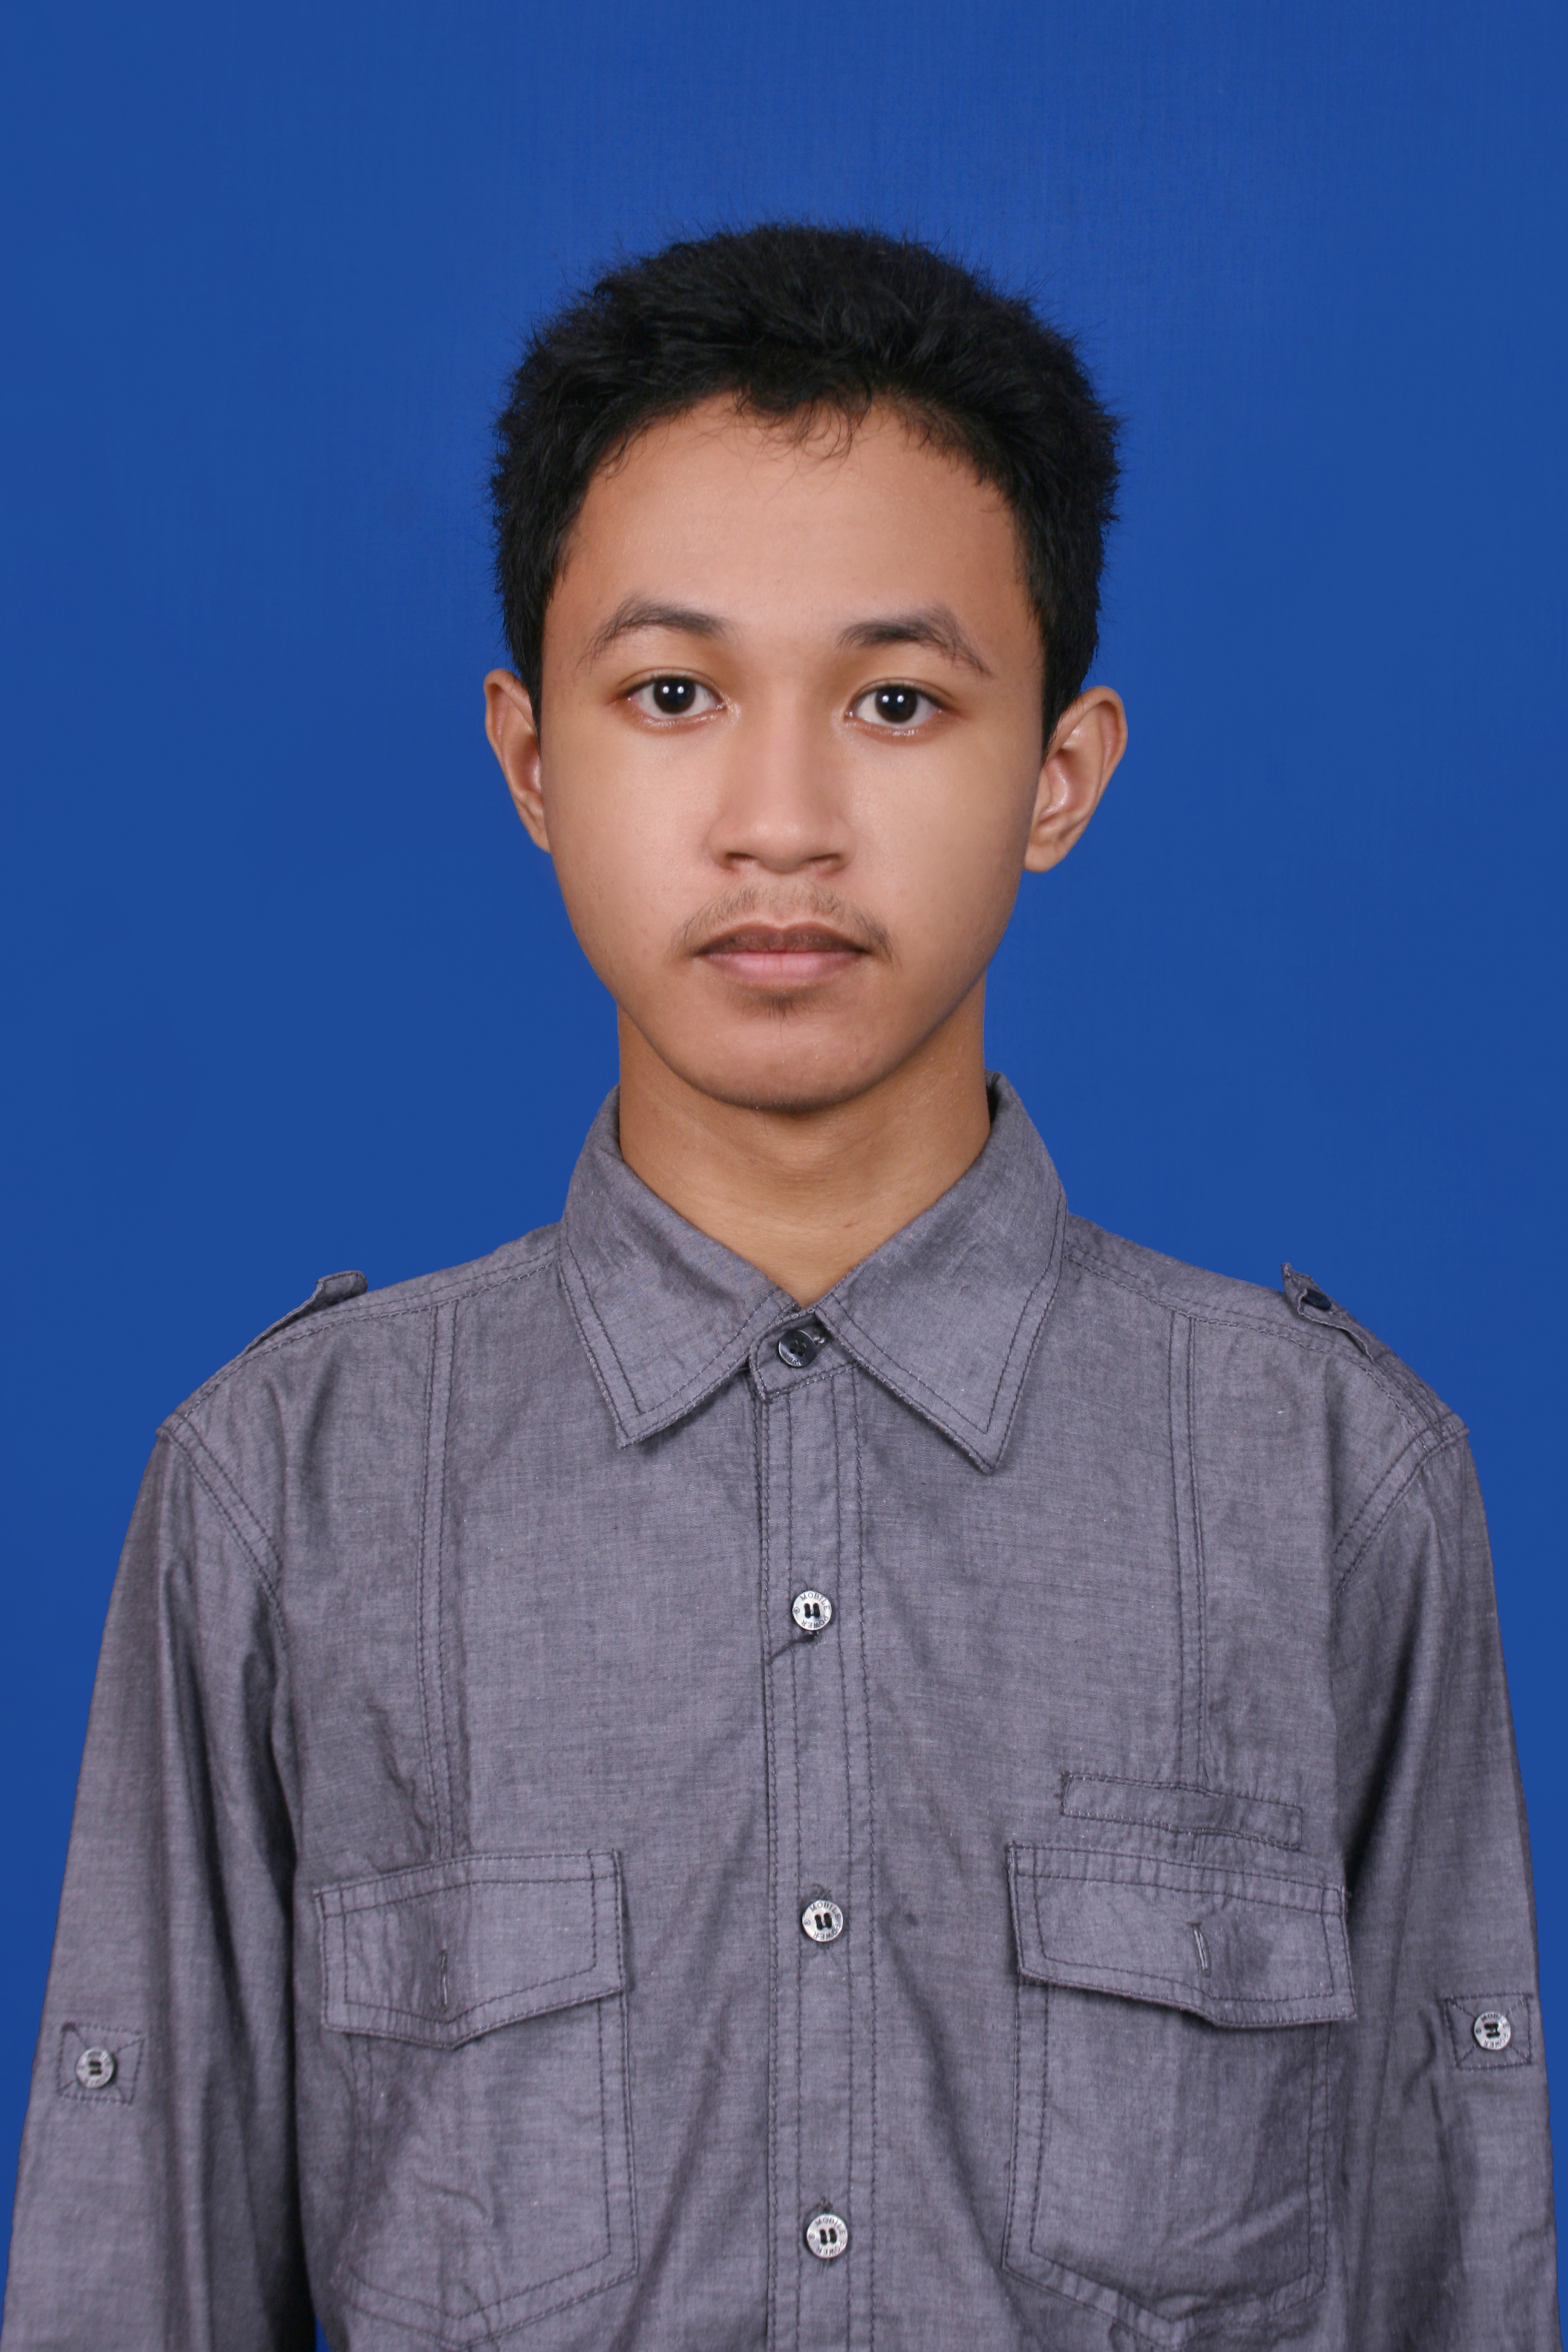
\includegraphics[height=0.3\textheight]{penutup/img/IMG_3563}
\end{wrapfigure}

Penulis bernama Muhammad Ghazian, putra ketiga dari empat bersaudara yang lahir pada tanggal 29 Desember 1995 di Bogor. Penulis telah mengenyam pendidikan di Sekolah Dasar Islam Terpadu Ummul Quro pada tahun 2002 hingga 2008, Sekolah Menengah Pertama Negeri 1 Bogor pada tahun 2008 hingga 2011, dan Sekolah Menengah Atas Neger 2 Bogor pada tahun 2011 hingga 2014. Pada masa penulisan, penulis sedang menempuh masa studi S1 di Institut Teknologi Sepuluh Nopember, Surabaya di \jurusanlama.

Selama masa studi, penulis memiliki ketertarikan yang dalam mengenai \textit{Artificial Intelligence}, rancang bangun aplikasi \textit{game}, dan rancang bangun aplikasi sistem informasi. Keinginan penulis dalam mengajar juga mendorong penulis menjadi asisten dosen pada mata kuliah Dasar Pemrograman, Struktur Data, Perancangan dan Analisis Algoritma (I), dan Perancangan dan Analisis Algoritma (II). Karya penulis semasa perkuliahan diantaranya adalah pembangunan Sistem Penilaian Unit Angka Kredit Guru untuk Kementerian Pendidikan Provinsi Jawa Timur. Selain itu, penulis juga cukup aktif membuat \textit{game} di sela-sela waktu kosong.

Di luar kesibukan akademik, penulis cukup aktif di lembaga dakwah jurusan sebagai salah satu staf. Penulis juga berkontribusi dalam berbagai kepanitiaan, baik dalam skala kecil (yaitu dalam kampus) maupun skala nasional. Kegiatan terakhir penulis adalah membantu kegiatan pelatihan nasional bagi peserta Olimpiade Komputer Indonesia pada Februari dan Maret 2018 lalu.


\end{document}